\documentclass[a5paper]{ufsc-thesis}

% UTF-8
\usepackage[utf8]{inputenc}
% Fonte
\usepackage[T1]{fontenc}
\usepackage{lmodern}
% Português
\usepackage[brazil]{babel}


%%% BIBLIOGRAFIA %%%
% Indicar páginas com as citações na bibliografia
%\usepackage[brazilian,hyperpageref]{backref}
% Citações padrão ABNT
\usepackage[alf]{abntex2cite}


%%% OUTRAS PACOTES %%%
% Matemática
\usepackage{amsmath}
% TikZ
\usepackage{tikz}
\usetikzlibrary{positioning}
% Novos comands
\usepackage{xparse}
% Sub-figuras
\usepackage{subcaption}


%%% NOVOS COMANDOS %%%
% Destaque - coisas a tratar
\newcommand \tratar[1] {\textcolor{red}{!!! #1 !!!}}
% Notação O
\DeclareMathOperator \bigO {O}
\newcommand \Oalt {$\bigO(\mathit{altura})$}
% ...
\newcommand \no[1] {$#1$}
\DeclareMathOperator \pai {pai}
\newcommand \id[1]    {\ensuremath{\mathrm{id}_{#1}}}
\newcommand \idstr[1] {\ensuremath{\id{#1}^{\mathrm{str}}}}
\newcommand \fACMP {$\mathrm{ACMP}$}
\newcommand \ACMPIDs {$\mathrm{ACMP}_{\mathrm{IDs}}$}


%%% ALGORITMOS %%%
\usepackage{algpseudocode}
\usepackage{algorithm}
\floatname{algorithm}{Algoritmo}
\newcommand \var[1] {\mathrm{#1}}
\newcommand \Cmnt[1] {\textcolor{green!50!black}{// #1}} %alg
\DeclareMathOperator \OuExBit {\mathbf{OuEx_{bit-a-bit}}}
\DeclareMathOperator \EBit {\mathbf{E_{bit-a-bit}}}


%\usepackage{cmap} ???


\usepackage[printonlyused]{acronym} 

% Preâmbulo
\titulo{REPRESENTAÇÃO OTIMIZADA DE TOPOLOGIAS DE MÁQUINA}
\autor{Igor da Silva Solecki}
\data{\today}
\instituicao{Universidade Federal de Santa Catarina}
\local{Florianópolis, SC}
\tipotrabalho{TCC}
\orientador{Prof. Dr. Laércio Lima Pilla\\Universidade Federal de Santa Catarina}
\programa{Programa de Graduação em Ciências da Computação}
\preambulo{Trabalho de Conclusão de Curso submetido ao Curso de Bacharelado em Ciências da Computação para a obtenção do Grau de Bacharel em Ciências da Computação.}
\centro{Centro Tecnológico -- CTC}
\assuntos{Ciências da Computação,Modelos,Teses,OpenSource,LaTeX}


\begin{document} %%%

%%%%%%%%%%%%%%%%%
%%% PRÉ-TEXTO %%%
%%%%%%%%%%%%%%%%%

% Inicia parte pré-textual do documento capa, folha de rosto, folha de
% aprovação, aprovação, resumo, lista de tabelas, lista de figuras, etc.
\imprimircapa
\imprimirfolhaderosto*

\begin{siglas}
	\item[tst] tst \cite{Sequoia}
	\item[etc] ...
\end{siglas}

%\include{init/pretextuais}
%\clearpage
%\imprimirfichacatalografica
%\tableofcontents


%%%%%%%%%%%%%%%%%
%%%   TEXTO   %%%
%%%%%%%%%%%%%%%%%
\textual

\chapter{Introdução}
\label{cap:introducao}
\acresetall


Atualmente, arquiteturas de computadores são construídas de forma hierárquica quanto à memória.
Essa hierarquia diz respeito à passagem de dados entre os diferentes níveis, ou seja, quais caminhos existem para que dados sejam comunicados entre pontos dessa hierarquia.
O que motiva sua existência é o fato de que diferentes tipos de memória possuem tamanhos, velocidades de acesso e custos distintos, e ela permite que o espaço das memórias maiores esteja disponível sem que se perca a velocidade das menores e mais rápidas \cite{Patterson}.
Níveis de memória mais baixos possuem maior capacidade de armazenamento, porém seu tempo de acesso é maior.
Parte dessa hierarquia é composta por um ou mais níveis de cache, memórias com capacidade reduzida, mas maior velocidade, permitindo que, em um dado momento, um conjunto de dados qualquer possa ser acessado mais rapidamente.
No nível mais alto dessas hierarquias estão as unidades de processamento, acessando e operando sobre os dados em memória.
Quanto mais próximo for o nível de memória em que esse dados estiverem, menor o tempo de acesso.
Quando essas unidades precisam se comunicar entre si, elas fazem uso da hierarquia de memória.

A hierarquia pode ser organizada de várias formas, podendo se tornar complexa e de grande profundidade.
Uma possibilidade na organização é o compartilhamento de alguns níveis de cache, ou seja, duas unidades de processamento ou mais estarão acima de uma mesma cache na hierarquia.
Isso permite, por exemplo, realizar comunicações com eficiência, pois o tempo entre algum dado ser atualizado e o novo valor ser visto é determinado pelo tempo de acesso à cache compartilhada.
Uma grande variedade de organizações pode ser encontrada ao se considerar arquiteturas como multicore, em que várias unidades de processamento chamadas de núcleos (\textit{cores}) fazem parte de um mesmo circuito integrado, ou \ac{numa}, em que mais níveis são acrescentados à hierarquia, compondo a rede de interconexão. Esta rede, por si só, também pode ser organizada de várias formas distintas.
Essa organização compreendendo hierarquia de memória e unidades de processamento, na sua totalidade, define uma topologia de máquina.

A necessidade de plataformas para rodar aplicações de alto desempenho tem dado origem às diversas arquiteturas paralelas modernas existentes.
Suas topologias são as mais variadas, visando atender às necessidades de várias classes de aplicações com características e comportamentos distintos.
Diante da crescente complexidade das topologias dessas máquinas, as suas organizações e as demais características dos elementos que compõe a hierarquia de memória são aspectos de muita relevância para o desempenho de aplicações.

Certas combinações de fatores da aplicação e da arquitetura podem resultar na melhoria ou na degradação do desempenho.
Tais fatores podem ser, por exemplo, a quantidade de dados manipulados e o tamanho das caches, que podem comportar ou não todos os dados simultaneamente, ou os padrões de troca de mensagens entre tarefas e a localização delas, além dos meios existentes para realizar essas comunicações, que podem resultar em maior ou menor eficiência \cite{Sequoia}. Um estudo de caso apresentado por \citeonline{LIKWID} mostra como uma certa distribuição de tarefas faz o desempenho cair aproximadamente pela metade.

Ainda, em arquiteturas NUMA, nas quais a memória é composta de várias partes que estão diretamente ligadas a nós distintos, de modo que diferentes regiões da memória possuem diferentes tempos de acesso, é importante que haja proximidade entre os dados acessados por uma thread e o núcleo em que ela reside.
Portanto, é essencial o conhecimento da topologia da máquina, que possibilita o devido ajuste das aplicações a ela, de modo a aproveitar ao máximo os recursos disponíveis.

Disso vem a necessidade de haver alguma representação da topologia para fornecer as informações necessárias sobre ela, seja diretamente às aplicações ou a outras partes do sistema, que usarão tais informações para realizar otimizações estática ou dinamicamente.
Como exemplo de uso estático, pode-se citar compilação de algoritmos com conhecimento da hierarquia \cite{Sequoia}, ou posicionamento de processos MPI \cite{hwloc2010}; e, quanto ao uso dinâmico, posicionamento de threads e dados OpenMP \cite{FGOMP}.

%[hwloc2010] http://www.open-mpi.de/papers/pdp-2010/hwloc-pdp-2010.pdf
%[FGOMP] https://hal.inria.fr/inria-00496295/document

No entanto, a disponibilização de tais informações gera custos adicionais, além de ter outras implicações relacionadas ao tamanho das estruturas de dados que podem afetar o desempenho.
Assim, é necessário que haja um compromisso entre o tempo de acesso e o espaço ocupado pela representação utilizada.
Tempos de acesso muito grandes podem acabar anulando os ganhos das otimizações.
Já se as estruturas de dados forem muito espaçosas, pode ser que não possuam boa localidade espacial, dependendo dos padrões de referência aos dados em acessos consecutivos.
Isso pode resultar em perda de desempenho ocasionada por faltas de cache, tanto no acesso às informações da topologia quanto no acesso pelas aplicações aos seus próprios dados.
Entretanto, é possível que a adição de algumas informações facilitem certas consultas sobre a topologia sem causar tais prejuízos, que é o desejado.



\section{Motivação}
\label{sec:motivacao}

Os exemplos de usos estáticos e dinâmicos dados acima, além de vários outros existentes, com o uso de benchmarks, servem como justificativa para a realização de esforços para desenvolver reprentações com as características citadas, isto é, bom tempo de acesso e uso eficiente da memória.

Para as aplicações, o ideal é que os dados estejam sempre nos níveis de cache os mais próximos possíveis, de modo que seu uso nas computações seja mais eficiente.
Diante disso, compilação com conhecimento da hierarquia \cite{Sequoia} se vale do fato de que frequentemente problemas podem ser dividos em problemas menores de tamanho variável, e ajustar esses tamanhos à capacidade das caches torna o uso delas mais efetivo, pois todos os dados usados nessas partes menores da computação caberão nelas.
Ainda, quando é possível haver vários níveis de subdivisão do problema, formando também uma espécie de hierarquia de subdivisões, os tamanhos das partes em diferentes níveis podem ser ajustados aos níveis de cache consecutivos.
Isso pode ser visualizado com facilidade no exemplo de multiplicação de grandes matrizes presente no artigo referenciado.

A velocidade de níveis de cache mais próximos também beneficia a comunicação.
Isso pode ser visto no uso de \ac{mpi}, um padrão utilizado no desenvolvimento de programas paralelos que seguem o modelo de passagem de mensagens.
Em conjunto com dados sobre os padrões de comunicação entre processos, as informações sobre compartilhamento de caches podem ser usadas para definir um posicionamento de processos MPI que favoreça as comunicações \cite{hwloc2010}.
Outra otimização possível é o uso de metódos específicos do hardware para realizar comunicações dentro de um nó.

No contexto de arquiteturas NUMA, para diminuir o número de acessos a memórias remotas, há a possibilidade de mover os dados para outro nó ou as threads para outros núcleos.
Uma combinação dessas opções foi desenvolvida no ForestGOMP \cite{FGOMP}, uma extensão de uma implementação de OpenMP, padrão utilizado no desenvolvimento de programas paralelos para sistemas com memória compartilhada.
Seguindo o princípio de realizar essa combinação com base nos níveis da topologia, o posicionamento dinâmico de threads e dados desenvolvido no ForestGOMP se mostrou efetivo.
Um cenário apresentado é a existência de vários conjuntos de threads e dados com grande afinidade, em que a migração de uma thread para outro núcleo só ocorreria se houvesse um nível de cache compartilhado, de modo a manter a thread próxima dos seus dados, enquanto em outros casos poderia haver a migração de todas as threads e dados relacionados.

Esses exemplos ilustram como informações sobre a hierarquia podem efetivamente ser usadas para melhorar o desempenho de aplicações que seguem modelos ou estratégias em uso real, ou seja, os benchmarks utilizados possuem características encontradas na solução de problemas reais.
Isso diz respeito a, por exemplo, padrões de comunicação ou distribuição de carga, que podem apresentar irregularidades e outras características presentes em aplicações científicas de diversas áreas.



\section{Objetivos}
\label{sec:objetivos}

Este trabalho tem como objetivo o desenvolvimento de uma representação de topologias de máquina, compreendendo as estruturas de dados utilizadas e os métodos de acesso, que mantenha o compromisso necessário entre tempo de acesso e espaço ocupado na memória pelas estruturas de dados.

\subsection{Objetivos Específicos}
\label{subsec:objetivos_especificos}

Os objetivos específicos são:
\begin{itemize}
	\item Analisar fatores relevantes para a eficiência na representação de topologias
	\item Desenvolver representações (estruturas de dados e métodos de acesso)
	\item Testar as representações desenvolvidas, por meio de experimentos em diferentes máquinas, observando o uso da memória e o tempo de execução
	\item Disponibilizar uma nova ferramenta para a representação de topologias de máquina
\end{itemize}



\section{Metodologia}
\label{sec:metodologia}

\begin{itemize}
	\item Estudar organização de computadores com foco na hierarquia de memória
	\item Estudar como topologias de máquina são representadas em trabalhos e ferramentas do estado da arte
	\item Entender o protótipo utilizado no \ac{ecl} até o momento
	\item Implementar novos métodos de armazenamento e acesso às informações
	\item Testar os novos métodos e estruturas de dados utilizando máquinas com topologias diferentes e avaliar os resultados
\end{itemize}



\section{Organização do Trabalho}
\label{sec:organizacao_do_trabalho}

As seções restantes estão organizadas da seguinte forma:
No capítulo \ref{cap:fundamentacao_teorica}, serão apresentados alguns conceitos fundamentais relevantes para o trabalho.
No capítulo \ref{cap:estado_da_arte}, será fornecida uma visão geral do estado da arte em representação de topologias de máquina.
No capítulo \ref{cap:andamento_do_trabalho} constam o progresso atual do trabalho e o planejamento do seu prosseguimento.




% \section{ORGANIZAÇÃO DO TRABALHO} % (fold)
% \label{sec:organiza_o_do_trabalho}
% Este trabalho está organizado da seguinte forma:
% No ca\-pí\-tu\-lo \ref{cha:conceitos_fundamentais} serão apresentados os conceitos fundamentais para a compreensão desta monografia.
% No capítulo \ref{cha:revisao_bibliografica} será feita uma revisão de trabalhos correlatos.
% No quinto capítulo serão apresentados os resultados deste trabalho, bem como os pos\-sí\-veis trabalhos futuros.

% section organiza_o_do_trabalho (end)


%O projeto e validação dos \acp{ci} ... ferramentas de \ac{eda}, mostrado de maneira simplificada na Figura \ref{fig:fluxoProjeto}. ... em \textit{software} e \textit{hardware} e a arquitetura da parte de \textit{hardware} é definida. A seguir, é criada a descrição no \ac{rtl}, ... do \ac{ci}. 

%\begin{figure}[ht]
%    \centering
    %\includegraphics[width = \linewidth]{images/majorStepsOfHardwareDesign}
%    \includegraphics[width = \linewidth]{images/TopDownHardwareFlow_guntzel}
%    \caption{ Principais etapas no fluxo de projeto de  cirvuitos \textit{Very-Large-Scale Integration} (VLSI).\\ Adaptado de \citeonline{KahngLivro} p. 7.}
%    \label{fig:fluxoProjeto}
%\end{figure}

%A Figura \ref{fig:fluxoProjeto} descreve, de forma simplificada, o desenvolvimento \textit{top-down} de um \ac{ci}. O processo de concepção de um \ac{ci} em grande escala é altamente complexo. Ele pode ser dividido em passos distintos \cite{KahngLivro}. Este fluxo de projeto começa com uma especificação da arquitetura, com maior nível de abstração, descrevendo funcionalidades e temporizações do circuito antes de nível \ac{rtl}. Passa por etapa de síntese lógica e mapeamento para uma determinada tecnologia. Então a etapa de síntese física gera o leiaute do chip, bem como as interconexões das células e suas posições. Na etapa de fabricação, os leiautes são mandados para a manufatura. Por fim os chips são testados e encapsulados para sua utilização \cite{coussy2010high}.

%\section{ETAPA DE SÍNTESE FÍSICA}
%\label{sec:etapa_de_sntese_fisica}


%... bibliotecas de \textit{standard cells} \cite{KahngLivro}.

%Segundo \citeonline{KahngLivro} ... Figura \ref{fig:fluxoProjeto}.

%os locais dos blocos com IP (Propriedade Intelectual)\footnote{Blocos com propriedade intelectual são partes do circuito em que não se tem o direito de alterar seu leiaute ou interconexões internas.} e portas externas ou blocos macro.

%.. detalhado na seção \ref{sec:etapa_de_sintese_da_rede_de_distribuicao_de_relogio}.

%... serão explanados na Seção \ref{sec:restricao_setup_hold}.
%Esta fase é responsável por sintetizar a rede de distribuição de relógio. O objetivo de toda rede de distribuição de relógio (CDN) é a distribuição de um sinal de relógio respeitando as restrições temporais como \textit{setup}\footnote{\textit{Setup:} quantidade de tempo que um sinal precisa estar estável antes da transição de relógio. Ver Seção \ref{sec:restricao_setup_hold}} e \textit{hold}\footnote{\textit{Hold:} quantidade de tempo que um sinal precisa estar estável após da transição de relógio. Ver Seção \ref{sec:restricao_setup_hold}}, minimizando o \textit{skew}\footnote{\textit{Skew} é a máxima diferença nos tempos de chegada do sinal de relógio entre dois \textit{sinks}.} e o \textit{jitter}\footnote{\textit{Jitter} é a variação de um sinal em relação ao tempo.}.


%... reformulação do projeto \cite{Guthaus_Wilke}.
% Para satisfazer a inequação de \textit{setup} (equação \ref{eq.setup}), podemos aumentar o período ($T_{cyc}$), porém uma violação no tempo de \textit{hold} (equação \ref{eq.hold}) não pode ser corrigida, implicando muitas vezes em reformulação do projeto \cite{Guthaus_Wilke}.

%árvore com ligações cruzadas \cite{Yeh:2006}. 

%No projeto de \ac{vlsi}, ... de forma pictórica na Figura \ref{fig:clock_hierarquia}, a mesma encontra sem escala.

%\begin{figure}[ht]
%    \centering
%    \includegraphics[scale = .8]{images/clock_hierarquia}
%    \caption{Típica arquitetura da Rede de Relógio global, regional e local. Sem escala. Fonte: \cite[Revisiting Automated Physical Synthesis of High-Performance Clock Networks]{Guthaus_Wilke}}
%    \label{fig:clock_hierarquia}
%\end{figure}

%\subsection{DISTRIBUIÇÃO GLOBAL E REGIONAL}
%\label{ssub:distribuicao_global_e_regional}

%\subsection{DISTRIBUIÇÃO LOCAL}
%\label{ssub:distribuicao_local}

%... ou mais elementos sequenciais \cite{Kozhaya:2011, Xanthopoulos:2001}.

%Mais detalhes serão explanados na seção \ref{sec:skew}.} associado as mesmas. Para melhorar o posicionamento global, utiliza-se incrementalmente as estimativas da mesma e reposiciona-se os blocos, repetindo estas etapas por um número fixo de vezes.

%\section{OBJETIVOS}
%\label{sec:objetivos}

%\subsection{OBJETIVOS GERAIS} % (fold) OBJETIVO GERAL
%\label{ssub:objetivos_gerais}

%\subsection{OBJETIVOS ESPECÍFICOS}
%\label{ssub:objetivos_especificos}

% 	\begin{itemize}
% 		\item Implementar o algoritmo Method of Means and Medians \cite{Michael90}
% 		\item Implementar o algoritmo Recursive Geometric Matching \cite{Kahng1991_RGM}
% 		\item Implementar o algoritmo Deferred-Merge Embedding \cite{Boese1992_DME}
% 		\item Avaliar os algoritmos utilizando a infraestrutura da Competição de CAD do ICCAD2015 \cite{iccad_kim2015}, comparando o \textit{wirelength} e \textit{skew} com o algoritmo \textit{FLUTE} \cite{flute}, o qual foi adotado na referida infraestrutura.
% 		\item Utilizando a infraestrutura da Competição de CAD do ICCAD2015 \cite{iccad_kim2015}, comparar os três algoritmos entre si em termos de \textit{wirelength} e \textit{skew}. Comparar também os três algoritmos com o algoritmo \textit{FLUTE} \cite{flute}
% 	\end{itemize}

% subsubsection objetivos_especificos (end)
% section objetivos (end)

%\section{MÉTODO DE PESQUISA} % (fold)
%\label{sec:metodo_de_pesquisa}
%Inicialmente, serão realizados estudos sobre trabalhos científicos na literatura correlata, bem como estudos sobre o fluxo do desenvolvimento de \acp{ci}. A partir do conhecimento adquirido através do estudo da área, serão implementados e avaliados os três algoritmos (\textit{MMM, RGM, DME}). Os algoritmos serão implementados em linguagem de alto nível (C++) e utilizando infraestrutura disponível no \ac{ecl}. Posteriormente, será feita uma avaliação experimental sobre estes algoritmos.
% Estes passos metodológicos podem ser visualizados no fluxograma abaixo \ref{fig:fluxograma_metodo_pesquisa}.

%A Figura \ref{fig:fluxograma_avaliacao_experimental} apresenta ... implementados:
%\begin{itemize}
%	\item \textbf{Identificação do conjunto de registradores da árvore de relógio local:} este passo consiste em identificar quais elementos síncronos pertencem a  mesma região do \ac{lcb}\footnote{\ac{lcb} são os \textit{buffers} que fornecem o sinal de relógio das árvores regionais de relógio para as árvores locais de relógio. Mais detalhes serão explanados no capítulo \ref{cha:conceitos_fundamentais}.}. \textbf{Entrada:} circuito (\textit{bechmark}) utilizado no \ac{iccad} (2015). \textbf{Saída:} conjunto de elementos sequenciais de um mesmo \ac{lcb}.

%	\item \textbf{Roteamento das árvores de relógio locais utilizando algoritmos clássicos:} nesta etapa, serão implementados os três algoritmos clássicos \ac{mmm} de \citeonline{Michael90}, \ac{rgm} de \citeonline{Kahng1991_RGM} e \ac{dme} de \citeonline{Boese1992_DME}. Estes algoritmos vão ser adicionados na infraestrutura do \ac{iccad} Contest (2015) \cite{iccad_kim2015}. \textbf{Entrada:} conjunto de elementos sequenciais de um mesmo \ac{lcb}. \textbf{Saída:} grafo das interconexões da árvore local de relógio.
	
%	\item \textbf{Extração dos dados para comparação:} este passo consiste em calcular as estimativas de comprimento de interconexões e \textit{skew} pertencentes ao roteamento das árvores de relógio locais geradas no passo anterior. Estas estimativas serão avaliadas e comparadas no passo subsequente. Para se obter o comprimento das interconexões, é somado o comprimento de todas as interconexões presentes na árvore local de relógio. Para determinação do \textit{skew}, será utilizada a equação \ref{eq.skew}. \textbf{Entrada:} grafo das interconexões da árvore local de relógio. \textbf{Saída:} \textit{wirelength} e \textit{skew} da árvore local de relógio.
	
%	\item \textbf{Comparação dos resultados:} nesta etapa serão confrontados os resultados gerados pelo algoritmo FLUTE de \citeonline{flute}, com os algoritmos \ac{mmm}, \ac{rgm} e \ac{dme}. \textbf{Entrada:} comprimento das interconexões e \textit{skew} da árvore local de relógio. \textbf{Saída:} análise dos resultados. %detalhada no Capítulo \ref{cha:esperimentos_realizados}.
%\end{itemize}

%\begin{figure}[ht]
%    \centering
%    \includegraphics[width=\textwidth]{images/fluxograma_avaliacao_experimental_comparativo}
%    \caption{Fluxograma da Avaliação Experimental.}
%    \label{fig:fluxograma_avaliacao_experimental}
%\end{figure}

% chapter introducao (end)
\chapter{Fundamentação Teórica}
\label{cap:fundamentacao_teorica}
\acresetall


%Uma parte muito importante das hierarquias a ser considerada em questões de desempenho são as memórias cache.
As hierarquias de memória possuem várias características que afetam o desempenho de aplicações e precisam, portanto, ser conhecidas ao se trabalhar com aplicações de alto desempenho.
Nas seções a seguir são apresentados alguns conceitos importantes nesse contexto, e, ao final, alguns conceitos relacionados a estruturas de dados relevantes.



\section{Memórias Cache}
\label{sec:memorias_cache}

Caches são memórias com o próposito de diminuir o tempo médio de acesso aos dados. Mais especificamente, é comum haver dois ou três níveis de cache entre as unidades de processamento e a memória principal. Elas são construídas com tecnologias que as tornam mais rápidas que outros níveis abaixo \cite{Patterson}. Porém, essa velocidade vem em troca de custo mais elevado. Por isso, elas têm espaço de armazenamento menor, além de que memórias maiores podem ter sua velocidade de acesso diminuída, o que também motiva a existência de vários níveis de cache.

O princípio de sua funcionalidade é manter à disposição dos programas, de forma rápida, aqueles dados dos quais eles precisam ou que estão usando no momento. Esses dados são disponibilizados conforme a capacidade de armazenamento da cache. Esta comumente é menor que o conjunto de todos os dados sobre os quais o programa opera, resultando na necessidade de remover alguns dados para acomodar outros.

\subsection{Localidade Espacial}
\label{subsec:localidade_espacial}

Quando um programa referencia determinada posição da memória, é comum que logo em seguida os dados nas posições de memória adjacentes sejam necessários também. Assim é definida a localidade espacial: endereços próximos tendem a ser referenciados um após o outro com pouco tempo de diferença \cite{Patterson}. As caches levam isso em conta para beneficiar as aplicações, trazendo dos níveis de memória abaixo não só o dado requisitado, mas também os dados que o rodeiam, constituindo um bloco. Assim, do ponto de vista da cache, a memória é uma sequência de blocos que, quando necessários, são carregados em algum espaço disponível, ou substituem um bloco carregado previamente se não houver espaços disponíveis.

Analisar as caches ajuda a entender por que um esquema que usasse estruturas muito espaçosas para reduzir a quantidade de operações e acessos poderia não funcionar bem.
No pior caso, acessos consecutivos poderiam ser todos a blocos diferentes, ocasionando o custo de trazer cada um para a cache e resultando na poluição da cache das aplicações, ou seja, diversos blocos com dados das aplicações seriam substituídos, tornando maior o tempo para acessá-los na próxima vez.


\section{\textit{Non-Uniform Memory Access}}
\label{sec:numa}

\textit{Non-Uniform Memory Access} (NUMA) é um tipo de multiprocessador com espaço de endereçamento único em que diferentes partes da memória estão mais próximas de alguns núcleos do que dos outros \cite{Patterson}.
Deste modo, o tempo de acesso depende do núcleo e da memória acessada.
Sistemas desse tipo possuem boa escalabilidade, pois é possível adicionar nós sem prejudicar o tempo de acesso dos núcleos às memórias mais próximas.
Estas características diferem das de outro tipo de multiprocessador existente, \textit{Uniform Memory Access} (UMA), em que o tempo de acesso independe do núcleo e da memória, e não há a vantagem de memórias locais com tempo de acesso reduzido.
Um problema com arquiteturas UMA é a contenção: vários núcleos disputam pelo barramento para acessar a memória, podendo fazer com que alguns fiquem ociosos enquanto esperam, diminuindo o desempenho.
Além disso, a escalabilidade é reduzida -- ao aumentar a quantidade de núcleos, o tempo de acesso à memória também cresce, seja qual for a região acessada, podendo se tornar inaceitável.

O modo como os nós NUMA são interconectados determina os custos de comunicação entre quaisquer dois núcleos em nós distintos.
Além disso, ele define os níveis que existirão a mais na hierarquia, ou seja, a sua profundidade.
Essas informações são de grande valia e devem ser fornecidas por representações da topologia com precisão.
Mesmo poucos níveis a mais na rede de interconexão podem resultar em diferenças de desempenho significativas \cite{MPITopFunc}.


% Seção de conceitos
\section{Estruturas de dados}

%Esta seção lista alguns conceitos tradicionais e outros que serão usados especificamente neste trabalho.
%Esta seção apresenta alguns conceitos que serão utilizados neste trabalho.

%Árvores (estrutura de dados) - representar hierarquias de memória
Uma \textit{árvore} é uma estrutura de dados que define uma hierarquia, logo, é conveniente para representar hierarquias de memória.

%Nós e ligações
Árvores são compostas por nós e ligações que relacionam esses nós.
Cada nó possui dados que dependem do que a árvore representa e de com que propósito ela será usada.
Cada ligação relaciona dois nós, um com papel de \textit{pai}, e o outro com papel de \textit{filho}.
Ou seja, uma ligação estabelece que um nó $a$ é pai de outro nó $b$, e, equivalentemente, que o nó $b$ é filho do nó $a$.

Em uma árvore, existe um único nó que não possui pai, o qual é chamado de \textit{nó raiz} (ou simplesmente \textit{raiz}).
Todos os demais nós possuem exatamente um pai.
%Cada nó conectado 
%Pode ter qualquer quantidade de filhos; se nenhum, folha.
Cada nó pode ter qualquer quantidade de filhos.
Se não possui nenhum, é chamado de \textit{nó folha} (ou \textit{folha}). %, caso contrário, de \textit{nó interno}.
%Filhos ordenados
Os filhos de um nó são ordenados.
Essa ordem não necessariamente reflete algum atributo ou característica daquilo que os nós estão representando.

%Para se realizar operações sobre essa estrutura de árvore
Para se realizar operações sobre essa estrutura de árvore, é possível seguir as ligações para descobrir os nós adjacentes (pai e filhos).
Visto que árvores geralmente são visualizadas com o nó raiz no topo, \textit{subir} uma ligação significa obter o pai de algum nó, e \textit{descer}, obter um dos filhos de um nó.
%O pai de um nó é obtido \textit{subindo} a ligação entre ele e seu pai
%Seguir(?) uma ligação

%Ancestral e descendente
%Ancestral - Todos os nós aos quais se pode chegar subindo ligações
Todos os nós que podem ser obtidos subindo, em sequência, uma ou mais ligações a partir de um nó são chamados de \textit{ancestrais} desse nó.
Semelhantemente, nós que podem ser obtidos apenas descendo ligações são \textit{descendentes}.
%Uma árvore não possui ciclos -- 
Nenhum nó é ancestral de si mesmo.

%Níveis (nível/profundidade de um nó)
Uma árvore é dividida em \textit{níveis}, cada um composto por um ou mais nós.
O nível 0 é composto pela raiz.
O nível $i$ é composto por todos os nós que podem ser obtidos descendo $i$ ligações em sequência a partir da raiz.
O nível em que um nó está é também chamado de sua \textit{profundidade}.
%Ordem?
%A ordem dos filhos de cada nó da árvore define implicitamente uma ordem em cada nível.

%O grau de um nó é a quantidade de filhos que ele possui
A quantidade de filhos que um nó possui é chamada de \textit{grau do nó}.
%- Grau de um nível: o maior entre os graus dos nós de um nível.
O maior entre os graus dos nós que compõe um nível é chamado de \textit{grau do nível}.
%É comum os graus de todos os nós de um nível serem iguais, mas, em hierarquias assimétricas(?), isso não ocorre.


%--- Encaixar ---

%Assimetria - hwloc
%Simetria - todas folhas no mesmo nível (e com graus diferentes?)

%Nós de um mesmo nível  graus diferentes


\chapter{Estado da Arte} % (fold)
\label{cap:estado_da_arte}
\acresetall


No estado da arte quanto à representação de topologias de máquina encontra-se o projeto Hardware Locality (hwloc) \cite{hwloc2010}.

O hwloc é um pacote de software amplamente utilizado para a representação de topologias de máquina com grande portabilidade.
Ele contém ferramentas de linha de comando, além de permitir que aplicações acessem as informações sobre a topologia por meio de uma API na linguagem C.



\section{Objetos}
\label{sec:objetos}

Objetos são uma abstração usada para representar todos os elementos presentes na topologia, tanto memória quanto núcleos.
A hierarquia de memória é modelada como uma árvore de objetos, onde cada nível contém objetos de apenas um tipo.
A topologia por completo é representada de forma mais detalhada por meio de várias ligações (ponteiros) entre objetos, conforme as suas relações na hierarquia.
Essas relações são definidas como:
\begin{itemize}
	\item Pai (\textit{parent}): nó pai na estrutura de árvore
	\item Filhos (\textit{children}): nós filhos na estrutura de árvore
	\item Irmãos (\textit{siblings}): nós com o mesmo pai
	\item Primos (\textit{cousins}): Objetos numa mesma profundidade (e, portanto, de mesmo tipo); todos os objetos que compõe um determinado nível (irmãos ou não) são primos
\end{itemize}
% TODO Criar macro
\begin{figure}[h]
	\caption{Relações entre objetos em topologias do hwloc. Fonte: \cite{hwlocImg}}
	\label{fig:relacoes}
	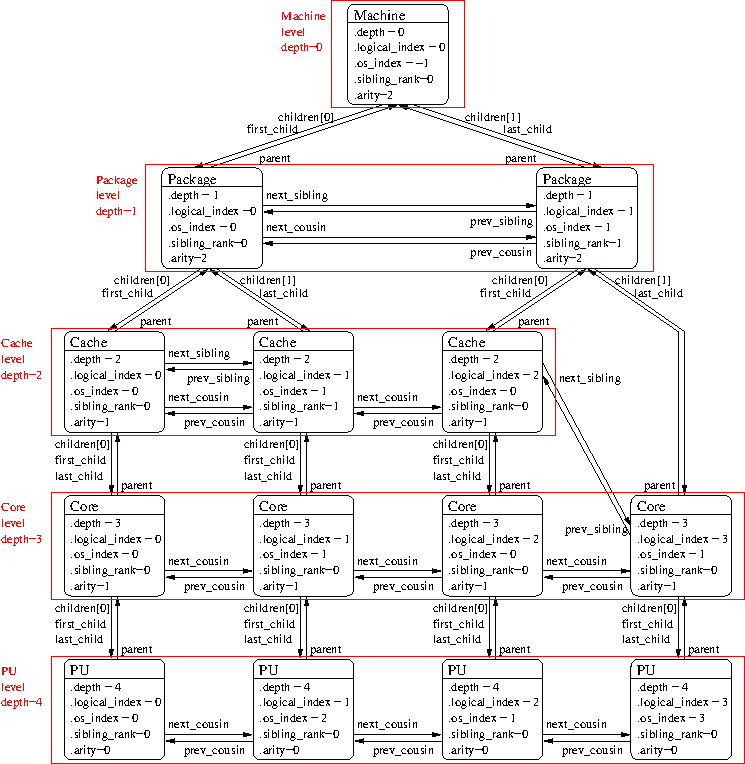
\includegraphics[width=\textwidth]{rec/img/relacoes}
\end{figure}
A Figura \ref{fig:relacoes} apresenta um exemplo dessas relações em uma dada topologia.
Ela ilustra, ainda, no ramo mais a direita, como hierarquias assimétricas (que possuem quantidades diferentes de objetos em ramos partindo do mesmo nó) são tratadas: podem surgir ``buracos'' devido a objetos de um mesmo tipo serem agrupados no mesmo nível.
% [Deixar mais claro] Buracos na hierarquia podem surgir porque o hwloc agrupa objetos do mesmo tipo no mesmo nível.
% Definir assimetria, segundo hwloc. Filhos com graus diferentes resulta em assimetria?
Portanto, objetos irmãos não estarão necessariamente no mesmo nível, e o conceito de profundidade não é exatamente o usado no contexto de estruturas de árvore, sendo possível irmãos terem profundidades diferentes.

Essas relações acrescentadas à estrutura de árvore facilitam a navegação entre objetos, em troca do espaço adicional ocupado por cada ponteiro nos objetos.
Por exemplo, como indicado na figura, a partir de qualquer objeto, é possível navegar para o próximo primo (pelo ponteiro \texttt{next\_cousin}), ou para o próximo irmão (ponteiro \texttt{next\_sibling}), se existirem.
Além disso, todos os objetos são armazenados numa estrutura de array de arrays de objetos, semelhante a uma matriz, mas com arrays internos de tamanho variável.
Cada um dos arrays internos contém os objetos de um nível, e eles são organizados no array externo na ordem dos níveis, de modo que é possível acessar o enésimo objeto de um dado nível diretamente usando essa estrutura.

%Figura X: https://www.open-mpi.org/projects/hwloc/doc/v1.11.2/diagram.png
Todos os objetos que compõe a hierarquia e outras estruturas de dados utilizadas na representação da topologia são armazenados em uma estrutura (\texttt{struct~hwloc\_topology}) que é utilizada pelas funções que acessam dados da topologia.


%?
\section{Funções e atributos}

Diversas funções podem ser utilizadas para acessar os objetos da hierarquia e informações sobre eles.
Alguns exemplos de funções são:
\begin{itemize}
	\item \texttt{hwloc\_get\_obj\_by\_type}: Informa quantos objetos de um determinado tipo existem, por exemplo, a quantidade de núcleos.
	\item \texttt{hwloc\_get\_cache\_covering\_cpuset}: Encontra a primeira memória cache que abrange um dado conjunto de CPUs.
	\item \texttt{hwloc\_get\_ancestor\_obj\_by\_type}: Encontra o ancestral de um dado objeto que seja de um determinado tipo.
	\item \texttt{\texttt{hwloc\_get\_ancestor\_obj\_by\_depth}}: Semelhante à função anterior, procurando por nível em vez de tipo.
	%\item \texttt{}:
\end{itemize}

Os objetos ainda têm atributos que podem guardar diversas informações, como detalhes do sistema operacional ou da máquina, que podem ser coletadas automaticamente durante o descobrimento da topologia ou adicionadas manualmente.
Além disso, há várias informações específicas de caches, como associatividade ou tamanho.
Também é possível associar estruturas arbitrárias aos objetos, conforme for necessário, usando dados de usuário (ponteiro \texttt{userdata}).


% >> Conjuntos de CPUs (cpusets)
\section{Conjuntos de CPUs}
\label{sec:conjuntos_de_cpus}

Cada objeto pode ter um \textit{cpuset} (conjunto de CPUs), que é um mapeamento dos núcleos existentes para bits (\textit{bitmap}), usado para determinar quais núcleos estão sob o objeto na hierarquia, implementado como uma sequência de variáveis de 32 bits, tantas quantas forem necessárias.
A implementação dos \textit{bitmaps} poderia ser otimizada para diminuir a quantidade de variáveis utilizadas em casos em que existam grandes quantidades de núcleos.
Algo nesse sentido é citado no respectivo arquivo fonte em um comentário sobre otimizações que poderiam ser realizadas \cite{hwlocCod}.
% Seção de conceitos
\section{Estruturas de dados}

%Esta seção lista alguns conceitos tradicionais e outros que serão usados especificamente neste trabalho.
%Esta seção apresenta alguns conceitos que serão utilizados neste trabalho.

%Árvores (estrutura de dados) - representar hierarquias de memória
Uma \textit{árvore} é uma estrutura de dados que define uma hierarquia, logo, é conveniente para representar hierarquias de memória.

%Nós e ligações
Árvores são compostas por nós e ligações que relacionam esses nós.
Cada nó possui dados que dependem do que a árvore representa e de com que propósito ela será usada.
Cada ligação relaciona dois nós, um com papel de \textit{pai}, e o outro com papel de \textit{filho}.
Ou seja, uma ligação estabelece que um nó $a$ é pai de outro nó $b$, e, equivalentemente, que o nó $b$ é filho do nó $a$.

Em uma árvore, existe um único nó que não possui pai, o qual é chamado de \textit{nó raiz} (ou simplesmente \textit{raiz}).
Todos os demais nós possuem exatamente um pai.
%Cada nó conectado 
%Pode ter qualquer quantidade de filhos; se nenhum, folha.
Cada nó pode ter qualquer quantidade de filhos.
Se não possui nenhum, é chamado de \textit{nó folha} (ou \textit{folha}). %, caso contrário, de \textit{nó interno}.
%Filhos ordenados
Os filhos de um nó são ordenados.
Essa ordem não necessariamente reflete algum atributo ou característica daquilo que os nós estão representando.

%Para se realizar operações sobre essa estrutura de árvore
Para se realizar operações sobre essa estrutura de árvore, é possível seguir as ligações para descobrir os nós adjacentes (pai e filhos).
Visto que árvores geralmente são visualizadas com o nó raiz no topo, \textit{subir} uma ligação significa obter o pai de algum nó, e \textit{descer}, obter um dos filhos de um nó.
%O pai de um nó é obtido \textit{subindo} a ligação entre ele e seu pai
%Seguir(?) uma ligação

%Ancestral e descendente
%Ancestral - Todos os nós aos quais se pode chegar subindo ligações
Todos os nós que podem ser obtidos subindo, em sequência, uma ou mais ligações a partir de um nó são chamados de \textit{ancestrais} desse nó.
Semelhantemente, nós que podem ser obtidos apenas descendo ligações são \textit{descendentes}.
%Uma árvore não possui ciclos -- 
Nenhum nó é ancestral de si mesmo.

%Níveis (nível/profundidade de um nó)
Uma árvore é dividida em \textit{níveis}, cada um composto por um ou mais nós.
O nível 0 é composto pela raiz.
O nível $i$ é composto por todos os nós que podem ser obtidos descendo $i$ ligações em sequência a partir da raiz.
O nível em que um nó está é também chamado de sua \textit{profundidade}.
%Ordem?
%A ordem dos filhos de cada nó da árvore define implicitamente uma ordem em cada nível.

%O grau de um nó é a quantidade de filhos que ele possui
A quantidade de filhos que um nó possui é chamada de \textit{grau do nó}.
%- Grau de um nível: o maior entre os graus dos nós de um nível.
O maior entre os graus dos nós que compõe um nível é chamado de \textit{grau do nível}.
%É comum os graus de todos os nós de um nível serem iguais, mas, em hierarquias assimétricas(?), isso não ocorre.


%--- Encaixar ---

%Assimetria - hwloc
%Simetria - todas folhas no mesmo nível (e com graus diferentes?)

%Nós de um mesmo nível  graus diferentes

\chapter{Implementação}
\label{cap:implementacao}

Esta seção apresenta as análises realizadas com foco no desempenho e os algoritmos e implementações resultantes.
Todo o código foi desenvolvido na linguagem C++.

Diante das considerações feitas sobre o projeto hwloc e o seu uso no projeto HieSchella, a função que encontra o ancestral comum mais próximo (\fACMP) entre dois nós foi escolhida como alvo de otimizações.
Ela é uma das funções implementadas no hwloc com complexidade \Oalt\ (ou $\bigO(\log N)$) e está entre as de uso mais significativo no HieSchella.
Na seção a seguir, será discutido como essa função poderia ser implementada de forma mais eficiente e quais as implicações de diferentes abordagens.


\section{Implementações da função \fACMP}

A função que encontra o ancestral comum mais próximo recebe dois nós como entrada (e possivelmente algumas estruturas adicionais, se houver necessidade)
e retorna um nó (o ancestral) como saída.
Cada par de nós em uma árvore tem exatamente um ancestral comum mais próximo.
%Existem algumas situações especiais.
Em geral, o caso em que os dois nós são o mesmo (\fACMP($a$,~$a$)) não será tratado.
Se um nó $a$ for ancestral de outro nó $b$, \fACMP($a$,~$b$) terá como resultado $a$.

\subsection{Abordagem inicial}

A maneira provavelmente mais intuitiva de se descobrir o ACMP é ``subir'' pela árvore, isto é, a partir dos dois nós dos quais se deseja encontrar o ACMP,
seguir as ligações em direção aos pais até se chegar ao mesmo nó.
Por ser um método que funciona subindo as ligações, será referido como método \Simples\ (Algoritmo~\ref{alg:simples}).
%que utiliza apenas a estrutura de árvore em si, sem adição de outras informações, será referido como método simples.
Sua complexidade é $\bigO(\log N)$.
Para que esse método funcione, é necessário subir de forma sincronizada -- a cada passo, devem-se comparar ancestrais dos dois nós iniciais que estejam no mesmo nível.
No caso do hwloc, o algoritmo se torna um pouco mais complicado, pois ele trata hierarquias assimétricas (pode haver ramos sem nó em algum nível).
Neste caso, mesmo que se tenham dois nós no mesmo nível, seus pais podem estar em níveis diferentes.
Ao fim de cada iteração, um dos nós pode estar ``mais alto'' (nível menor), portanto, este método usado pelo hwloc será chamado de \Hwloc\ (Algoritmo~\ref{alg:hwloc}), em analogia a uma superfície ondulada.
Um ponto que pode afetar o desempenho destes algoritmos é o fato de que é necessário acessar cada nó
(os nós iniciais e todos os seus ancestrais até o ACMP), e os nós estão espalhados pela memória.

% Simples (ascendente)
\begin{algorithm}
	\caption{ACMP Ascendente}
	\label{alg:simples}
	
	\Entrada{Dois nós $a$ e $b$}
	\Saida{O ACMP entre $a$ e $b$}
	\BlankLine
	
	\tcp{Inicialmente, encontra ancestrais de $a$ e $b$ no mesmo nível}
	\Enqto {$nível_a > nível_b$}
		{$a \gets \pai(a)$}
	\Enqto {$nível_b > nível_a$}
		{$b \gets \pai(b)$}
		
	\BlankLine
	\Enqto {$a \not= b$}
	{
		$a \gets \pai(a)$ \\
		$b \gets \pai(b)$ \\
	}
	\Retorna {$a$}
\end{algorithm}


% Hwloc (ondulado)
\begin{algorithm}
	\caption{\Hwloc\ -- \fACMP\ implementado no hwloc}
	\label{alg:hwloc}
	
	\Entrada{Dois nós $a$ e $b$}
	\Saida{O ACMP entre $a$ e $b$}
	\BlankLine
	
	\Enqto {$a \not= b$}
	{
		\Enqto {$\var{nível}_a > \var{nível}_b$}
			{$a \gets \pai(a)$}
		\Enqto {$\var{nível}_b > \var{nível}_a$}
			{$b \gets \pai(b)$}
		\Se {$a \not= b$ e $\var{nível}_a = \var{nível}_b$}
		{
			$a \gets \pai(a)$ \\
			$b \gets \pai(b)$ \\
		}
	}
	\Retorna {$a$}
\end{algorithm}


Considerando a estrutura de árvore apenas, a única informação que relaciona um nó aos seus ancestrais são as ligações.
% entre um nó e seus filhos (ou, no outro sentido, entre cada nó e seu pai).
%Assim, todas as sequências de uma ou mais ligações de filho para pai a partir de um nó (ou seja,
%entre o nó e seu pai, entre este e o pai dele, e assim por diante) definem os ancestrais do nó.
Isso indica que outras estruturas associadas aos nós ou à árvore como um todo se fazem necessárias
para ser possível encontrar o ACMP com algum método além dos mencionados.
Podemos considerar a seguinte ideia para encontrar outra maneira de implementar a função \fACMP:
Para uma dada árvore que representa uma topologia,
\begin{enumerate}
	\item Atribuir um valor (chamado de ID) a cada nó da árvore;
	\item Definir uma função \ACMPIDs\ que receba o ID de dois nós distintos e tenha como resultado o nó ACMP.
\end{enumerate}
Esses IDs (em conjunto com outras informações associadas a cada nó individualmente ou à árvore como um todo conforme necessário)
podem estabelecer alguma relação entre um nó e seus ancestrais além da que já existe por meio das ligações da árvore.

Idealmente, para implementar essa função \ACMPIDs, deveria ser encontrado um algoritmo de complexidade constante.
%que seja executado em tempo constante nos processadores modernos.
No entanto, é preciso lembrar que, mesmo que a quantidade de instruções executadas pelo processador seja constante,
a maneira como a memória é acessada pode aumentar o tempo de execução, especialmente quando há outras tarefas fazendo uso da memória, o que deve acontecer em cenários reais.

Com isso em mente, podemos analisar diferentes formas de definir tal função para descobrir qual seria mais adequada.
%definir tal função usando as operações básicas encontradas no conjunto de instruções das arquiteturas atuais,
%tais como as operações aritméticas e operações lógicas \textit{bit-a-bit}.

\subsection{Matriz}

Uma possibilidade é relacionar cada par de nós ao seu ACMP por meio de uma matriz
em que cada linha representa um nó da árvore, assim como cada coluna, e o cruzamento contém o ACMP entre o nó da linha e o nó da coluna.
Para isso, pode-se atribuir a cada um dos $N$ nós da árvore um ID único entre $0$ e $N-1$ e usar esses IDs como índices na matriz,
que terá, na posição $A(i,j)$, o ACMP entre o nó de ID $i$ e o nó de ID $j$.
No entanto, esta é uma estratégia ingênua, pois esse espaço $\bigO(N^2)$ ocupado na memória resultaria em problemas como sujar a \textit{cache} da aplicação.
A Tabela~\ref{tab:dif_arvore_matriz} sumariza a diferença entre a utilização de uma árvore e de uma matriz para a função \fACMP.
Visto que a matriz é simétrica, apenas cerca de metade dela precisa realmente ser armazenada.
Esta otimização foi utilizada na implementação dos testes de desempenho, conforme o Algoritmo~\ref{alg:matriz}.
Isso, no entanto, não altera a complexidade espacial.

% Tabela comparando árvore com matriz
\begin{table}[htb]
	\centering
	\caption{Complexidade das representações com árvore e com matriz}
	\label{tab:dif_arvore_matriz}
	\begin{tabular}{ccc}
		\toprule
		& Árvore & Matriz \\
		\midrule
		\begin{tabular}{@{}c@{}}Acesso\\(encontrar ACMP)\end{tabular}
			& $\bigO(\log N)$
			& $\bigO(1)$ \\
		\begin{tabular}{@{}c@{}}Espaço ocupado\\na memória\end{tabular}
			& $\bigO(N)$
			& $\bigO(N^2)$ \\
		\bottomrule
	\end{tabular}
\end{table}

% Matriz
\begin{algorithm}[h]
	\caption{\textsc{MatrizACMP} -- \fACMP\ usando uma matriz}
	\label{alg:matriz}
	
	\newcommand \linha {\mathrm{linha}}
	\newcommand \coluna {\mathrm{coluna}}
	
	\Entrada{Dois nós $a$ e $b$ \newline
	         Uma matriz $M$ que possui na linha $i$ e coluna $j$ ($M(i, j)$),
	          $i > j$, o ACMP entre os nós de ID $i$ e $j$}
	\Saida{O ACMP entre $a$ e $b$}
	
	%\BlankLine
	%\tcp{A matriz é simétrica, elementos acima da diagonal principal não são utilizados}
	
	\BlankLine
	%Matriz$\langle$Nó$\rangle$ $M$, Nó \no{a}, Nó \no{b}
	$\linha  \gets \max(\id{a}, \id{b})$ \\
	$\coluna \gets \min(\id{a}, \id{b})$ \\
	\Retorna $M(\linha, \coluna)$ \\
	%\EndFunction
	
\end{algorithm}


\subsection{Função de espalhamento}

Outra possibilidade foi idealizada, dividindo a função \ACMPIDs\ em dois passos:
\begin{enumerate}
	\item dados os IDs de dois nós, descobrir o ID do ancestral;
	\item encontrar o nó que possui esse ID.
\end{enumerate}
Em linhas gerais, o funcionamento do primeiro passo se baseia no seguinte:
%- O comprimento de um ID é a quantidade de \textit{bits} da sua representação em binário, descartando zeros à esquerda.
O ID de um nó aparece na representação binária dos IDs de todos os seus descendentes.
Desse modo, dados os IDs de dois descendentes, é possível identificar o ID do ACMP.
Usando apenas as operações que podem ser vistas nas linhas 1~--~4 do Algoritmo~\ref{alg:novo} mais adiante,
para as quais existem instruções que tomam poucos ciclos nas arquiteturas atuais, pode-se descobrir o ID do ACMP.
A quantidade de instruções é fixa, portanto, a complexidade é constante.
Essa estratégia será chamada de \Novo\ pelo modo como o ID do ancestral é extraído da parte dos IDs em que eles combinam.

Para descrever como os IDs são formados, as seguintes definições são necessárias:
\begin{itemize}
	\item \id{a} é o ID do nó $a$.
	\item \idstr{a} é uma cadeia (\textit{string}) de bits correspondente ao \id{a} em binário (com o bit menos significativo na última posição). O tamanho depende do nível de $a$, como será especificado adiante.
\end{itemize}
Os IDs, então, são definidos da seguinte forma:
\begin{itemize}
	\item A raiz tem id 0, e \idstr{\mathit{raiz}} é a cadeia vazia.
	\item Quanto aos demais, para cada nó $a$,
		$$\idstr{a} = x \parallel \idstr{pai(a)}$$
	onde $\parallel$ é a concatenação e $x$ é uma cadeia cujo tamanho é o grau do nível de $\pai(a)$.
	Se a é o i-ésimo filho de seu pai, $x$ possui 1 na i-ésima posição da direta para a esquerda e 0 nas demais.
\end{itemize}

Assim, as cadeias correspondentes aos IDs de todos os nós de um nível têm o mesmo tamanho, que é o somatório dos graus dos níveis anteriores.
A Figura~\ref{img:exemplo_ids} apresenta os IDs atribuídos aos nós de uma árvore.
O \tratar{Algoritmo X} mostra como o ID do ACMP é obtido a partir do ID de dois nós.

\begin{figure}
	\centering
	\caption{Exemplo de árvore com IDs atribuídos aos nós}
	\label{img:exemplo_ids}
	\begin{tikzpicture}[no/.style={draw, circle, minimum size=1cm, align=center}]
	%[estado/.style={circle,minimum size=1cm}]
	%\node [estado] (IUA)    at ({360/\n * (3+.5)}:\raio) {I U A};
		% Árvore
		\node [no] (a) {$a$}
			[level distance=2cm,
			level 1/.style={sibling distance=30mm},
			level 2/.style={sibling distance=15mm}]
			child {node [no] (b) {b}
				child {node [no] (e) {e}}
				child {node [no] (f) {f}} }
			child {node [no] (c) {c}
				child {node [no] (g) {g}}
				child {node [no] (h) {h}} }
			child {node [no] (d) {d}
				child {node [no] (i) {i}}
				child {node [no] (j) {j}} }
		;
		% IDs
		\newcommand \caa[1] {\textcolor{red!50!black}{#1}}
		\newcommand \cab[1] {\textcolor{red!50!red}{#1}}
		\newcommand \cac[1] {\textcolor{red!50!white}{#1}}
		\newcommand \cba[1] {\textcolor{blue!75!black}{#1}}
		\newcommand \cbb[1] {\textcolor{blue!75!white}{#1}}
		\DeclareDocumentCommand \labelId {m m m O{right} O{0}}
			{\node [align=center, node distance=#5, #4=of #1]
			{$\id{#1} = #2$\\$\idstr{#1} = #3$}}
		% Folha
		\DeclareDocumentCommand \labelIdF {m m m O{0}}
			{\labelId{#1}{#2}{#3}[below][#4]}
		% Folha mais baixa
		\DeclareDocumentCommand \labelIdFB {m m m}
			{\labelIdF{#1}{#2}{#3}[1]}
		\labelId{a}{0}{{\color{gray} (vazio)}};
			\labelId{b}{1}{\caa{001}};
				\labelIdF{e}{9}{\cba{01}\ \caa{001}};
				\labelIdFB{f}{17}{\cbb{10}\ \caa{001}};
			\labelId{c}{2}{\cab{010}};
				\labelIdF{g}{10}{\cba{01}\ \cab{010}};
				\labelIdFB{h}{18}{\cbb{10}\ \cab{010}};
			\labelId{d}{4}{\cac{100}};
				\labelIdF{i}{12}{\cba{01}\ \cac{100}};
				\labelIdFB{j}{20}{\cbb{10}\ \cac{100}};
	\end{tikzpicture}
\end{figure}
 % Explicação de como os IDs são formados

\begin{algorithm}
	\caption{\Novo\ -- \fACMP\ usando as novas estruturas}
	\label{alg:novo}
	
	\newcommand \imgN {E}
	
	\Entrada{Dois nós $a$ e $b$ \newline
	         %Opa \newline
	         Uma função \bpn, que retorna o nível
	          do ancestral comum entre dois nós
	          dado um número com apenas um bit 1,
	          na primeira posição em que o ID dos nós difere \newline
	         A função \textsc{Espalhamento} (Algoritmo \ref{alg:espalha})
	          com dados da árvore em questão \newline
	         Uma matriz (vetor de vetores) $\imgN$,
	          onde o vetor $\imgN(i)$ possui os nós do nível $i$
	          distribuídos pela função \textsc{Espalhamento}($i$, id)}
	\Saida{O ACMP entre $a$ e $b$}
	\BlankLine
	
	%Nota: Processadores atuais possuem uma instrução cujo resultado
	%      é a posição do primeiro bit 1 em um número,
	%      o qual pode ser usado para acessar um arranjo
	%\BlankLine
	
	\LinesNumbered
	%\Function{ancestral}{Estruturas $\var{E}$, No $a$, No $b$}
	%ID dif, bit, \var{masc}, id;
	\tcp{Bits que diferem}
	$\var{dif} \gets \id{a} \OuExBit \id{b}$ \\
	\tcp{Bit 1 apenas na primeira posição em que os IDs diferem}
	$\var{bit} \gets \var{dif} \EBit (-\var{dif})$ \\
	\tcp{Todos os bits antes do primeiro diferente}
	$\var{\var{masc}} \gets \var{bit} - 1$ \\
	%//\var{masc} = (((\var{dif}-1) ^ \var{dif}) >> 1);
	\tcp{Id do ancestral comum mais próximo}
	$\var{id} \gets \id{a} \EBit \var{masc}$ \\
	
	\BlankLine
	\tcp{Encontra o nó}
	$\var{nível} \gets \bpn(\var{bit})$ \\
	$\var{pos}   \gets \textsc{Espalhamento}(\var{nível}, \var{id})$ \\
	\Retorna $\imgN(\var{nível}, \var{pos})$ \\
	
	%\tcp{Arranjo com os nós já distribuídos pela função de espalhamento}
	%$\var{imagemNivel} \gets \mathrm{E.imagemNiveis}(nivel)$ \\
	%$\var{imagemNó} \gets
	%	\mathrm{E.dadosFuncao}[\var{nivel}].aplicar(\var{id})$ \\
	%\Retorna $\var{imagemNivel}[\var{imagemNó}]$ \\
\end{algorithm}

% Espalhamento
\begin{algorithm}
	\caption{\Espalha\ -- Função de espalhamento}
	\label{alg:espalha}
	
	\Entrada{Um nível (inteiro não negativo) $n$ \newline
	         O id de um nó}
	\Saida{A posição em que o nó deve ficar no vetor do seu nível}
	\BlankLine
	
	Nota: Os valores $\var{ad}_{n}$, $\var{m}_{n}$,
	                 $\var{mult}_{n}$ e $\var{desl}_{n}$
	      dependem da árvore com a qual se usará esta função
	      e do nível recebido ($n$).
	      $x \Desl b$ é o valor $x$ deslocado $b$ bits para a direita,
	      equivalente a $\lfloor x/(2^b)\rfloor$. \\
	\BlankLine
	
	\tcp{Minimiza o resultado ${}\bmod m_{n}$ para minimizar o tamanho do vetor}
	$\var{v} \gets \var{id} + \var{ad}_{n}$ \\
	\tcp{Equivalente a $\var{v} \bmod m_{n}$}
	\Retorna $\var{v} - ((\var{v} * \var{mult}_{n})
		\Desl \var{desl}_{n}) * m_{n}$ \\
\end{algorithm}


Falta, então, apenas o segundo passo, o de encontrar o nó a partir do ID.
Algumas opções para isso seriam:
\begin{itemize}
	\item Usar os IDs como índices em um arranjo: Seria simples, mas impraticável -- poderiam ser necessários arranjos com milhões de posições (devido a como os IDs são formados) e apenas algumas centenas ocupadas.
	\item Usar uma função de espalhamento (\textit{hash}): a maneira mais simples seria apenas aplicar a operação módulo com algum $m$ ($\mathrm{id} \bmod m$).
	No entanto, podem haver colisões (dois IDs diferentes podem ser congruentes módulo $m$).
	Isso pode ser tratado, mas acarretaria acessos adicionais à memória, o que não é desejável.
	Por exemplo, para os IDs do nível 1 da Figura~\ref{img:exemplo_ids}, $(1, 2, 4)$, $m = 3$ resultaria em $(1, 2, 1)$, com dois nós mapeados para a posição 1.
	\item Buscar uma função que não cause colisões: o mesmo que a função de espalhamento, porém utilizando um valor de módulo que não cause colisões.
	Pode exigir arranjos cujo tamanho é algumas vezes maior que a quantidade de nós, mas aparenta compensar quando comparado a tratar colisões de outros modos.
	Por exemplo, com os mesmos IDs, $m = 4$ resultaria em $(1, 2, 0)$, sem colisões (e, coincidentemente, exigiria um arranjo de apenas três posições).
	Este foi o método escolhido.
\end{itemize}

As linhas 5~--~7 do Algoritmo~\ref{alg:novo} apresentam como este método funciona.
Quanto à implementação da função \bpn, os processadores atuais possuem uma instrução que encontra a posição do primeiro \textit{bit} 1 em um número, a qual pode ser usada como índice em um pequeno arranjo contendo o devido resultado da função \bpn.
Se os IDs têm até $b$ \textit{bits}, esse arranjo precisar ter $b$ posições.
A função \Espalha\ (Algoritmo~\ref{alg:espalha}) utiliza dados específicos para a árvore, que devem ser descobertos previamente.

Testes feitos indicaram que a operação mais custosa no \Novo\ era o módulo, usado na função \Espalha.
No entanto, existem técnicas para realizar de maneira mais barata a divisão com denominador previamente conhecido \cite{reciproco}, e com o resultado da divisão pode-se calcular o módulo.
Essas otimizações são usadas, por exemplo, por compiladores, sendo chamadas de Redução de Força.
Aqui, no entanto, a ideia não é realizá-las em tempo de compilação, mas quando se está montando as estruturas para uma hierarquia específica.
Isso continua sendo vantajoso pois a montagem ocorre apenas uma vez e esta operação de módulo com o mesmo valor será realizada uma grande quantidade de vezes.
Portanto, é possível substituir a operação de módulo por outras operações que se mostraram mais baratas, a saber, duas multiplicações, um deslocamento e uma subtração.
%Com esta alteração, os tempos diminuiram consideravelmente, conforme mostra a tabela [X])

Para se encontrarem valores apropriados para a função \Espalha, são testados valores cada vez maiores para $m$, até que não haja colisões.
Ao se encontrar um $m$ válido, se busca um $\mathit{ad}$ que minimize o maior resultado de $(\mathrm{id} + \mathit{ad}) \bmod m$, minimizando o tamanho do arranjo usado.
Então, são descobertos os valores de $\mathit{mult}$ e $\mathit{desl}$, usando a técnica descrita em \citeonline{reciproco}, para evitar a operação de módulo.

%\tratar{Estruturas foram testadas}
A corretude das estruturas utilizadas na implementação do \Novo\ foi testada.
O programa de testes cria uma árvore e compara o resultado do \Simples\ com o do \Novo\ para algumas buscas, além de verificar se todos os nós estão realmente na posição retornada pela função \Espalha.
Também é causada uma mutação em uma árvore e é verificado se o erro é detectado por esse código de verificação.


%Detalhes de como os IDs são formados
%\tratar{Pode falhar se os dois nós de entrada são, na verdade, o mesmo nó. If resolve
%A Tabela~\ref{tab:compara} apresenta a comparação entre algumas características dos métodos discutidos.
O \Novo, assim como o \Hwloc\ e o \Matriz, trata corretamente hierarquias assimétricas, diferentemente do \Simples.
No entanto, ele possui uma limitação: % devido a como os IDs são formados:
A quantidade de \textit{bits} do ID de um nó pode chegar até o somatório dos graus de todos os níveis.
Se esta quantidade ultrapassar o tamanho de uma palavra (geralmente 32 ou 64 \textit{bits}), o método terá problemas, limitando as árvores que podem ser usadas.
Além disso, a técnica usada na função \Espalha\ para otimizar o módulo inclui uma multiplicação cujo resultado pode ter até cerca do dobro da quantidade de \textit{bits} do penúltimo nível (o último nível não possui espalhamento, pois seus nós nunca serão ACMP).
Como uma solução parcial, níveis de grau um podem ser omitidos na definição dos IDs, visto que seus nós também nunca serão ACMP.
Atribuindo a cada nó desses níveis e ao seu filho o mesmo ID, eles continuam podendo ser usados em buscas de ACMP.
Deste modo, o tamanho máximo seria o somatório dos graus de todos os níveis de grau diferente de 1.

%Isto pode ser contornado isto utilizando o resultado, por exemplo, se for possível acessar o resultado de 128 \textit{bits} de uma multiplicação de 64 \textit{bits} $\times$ 64 \textit{bits}.
%limitando o tamanho das árvores que podem ser usadas
%Não é necessário  atribuir os níveis de grau um, 
O método poderia ser adaptado para usar mais palavras se necessário, teoricamente deixando de ser $\bigO(1)$ e se tornando $\bigO(\log N)$, mas, na prática, nenhuma árvore deve ser tão grande que exija uma quantidade significativa.
%Funciona em casos de hierarquias assimétricas, simples não
%Limitação: Quantidade de \textit{bits} necessária - Solução parcial: 'Esconder' níveis cujos nós têm só um filho (níveis de grau um).}

O código implementado tem suporte à aplicação das operações \texttt{Ou} e \texttt{Ou-Exclusivo} ao ID no início da função \Espalha, com valores que também precisariam ser descobertos previamente, o que poderia reduzir ainda mais o tamanho dos arranjos usados. No entanto, devido a restrições de tempo, a busca desses valores não foi implementada.

% Seção sobre testes de desempenho

\chapter{Testes de desempenho}
%POR QUÊ

Com o objetivo de avaliar o desempenho do algoritmo desenvolvido, foram realizados testes
que permitiram comparar o desempenho das diferentes abordagens.
Foi medido o tempo tomado pelos algoritmos
ao se encontrar repetidamente o ACMP entre os nós folhas de uma árvore.
Com esses dados, analisados

Um programa foi desenvolvido, também na linguagem C++, para realizar os testes de desempenho.
Foi utilizada a funcionalidade de templates da linguagem para facilitar a definição equivalente dos testes para todos os algoritmos, mas ainda assim permitir que o compilador otimizasse as chamadas, evitando custos adicionais durante os testes devido à hierarquia de classes utilizada.
O programa depende da biblioteca do hwloc.
Os valores medidos são escritos em um arquivo no formato CSV (Valores Separados por Vírgula -- \textit{Comma-Separated Values})


\section{Máquinas utilizadas nos testes}

Os testes foram executados sobre duas máquinas (notebooks), que serão identificadas como Máquina A e Máquina B, para as quais o programa lstopo gera as representações de hierarquia apresentadas na Figura \ref{img:maquinas}. Estas representações revelam o tamanho das memórias cache, que podem ter efeito nos resultados dos testes. Ambas possuem o sistema operacional Windows 10. \tratar{Mais detalhes (processador)?}

\begin{figure}
	\centering
	\caption{Saída do programa lstopo sobre as máquinas utilizadas}
	\label{img:maquinas}
	\begin{subfigure}{.4\textwidth}
		\caption{Máquina A}
		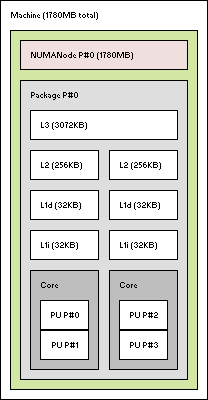
\includegraphics[width=\textwidth]{rec/img/MaqA}
	\end{subfigure}
	~
	\begin{subfigure}{.4\textwidth}
		\caption{Máquina B}
		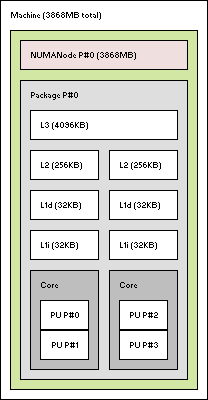
\includegraphics[width=\textwidth]{rec/img/MaqB}
	\end{subfigure}

\end{figure}

%COMO
\section{Estrutura dos testes}

Os testes consistem em encontrar repetidamente o ACMP entre os nós folhas de uma dada árvore com os diferentes algoritmos -- o existente no hwloc e os implementados.
Cada vez que as estruturas necessárias são criadas e os testes são executados sobre elas com um determinado algoritmo, obtém-se uma observação, que é o tempo que levou para realizar a quantidade especificada de repetições da função ACMP entre os nós folhas da árvore com o algoritmo.

Para cada algoritmo, uma árvore de estrutura equivalente é criada (as estruturas de dados dependem do algoritmo) a partir dos graus fornecidos como entrada.
%(Como os graus são usados para montar a árvore -- se não for explicado antes)
Os graus são recebidos como uma lista de inteiros positivos.
O i-ésimo será o grau do nível $i-1$.
Deste modo, se os graus recebidos são $(g_1, g_2, ..., g_n)$, a raiz terá $g_1$ filhos, cada um com $g_2$ filhos, e assim por diante, até os nós do nível $n-1$, que terão $g_n$ filhos cada.

Para obter uma observação de um algoritmo, uma lista contendo todos os pares possíveis de nós folhas (todas as combinações de duas folhas) é criada.
Esta lista é embaralhada, usando uma semente fixa, de modo que a ordem pseudo-aleatória é a mesma para todas as execuções de todos os algoritmos sobre esta árvore.

Uma observação é obtida por meio de uma etapa de aquecimento seguida de uma de medição, na qual o tempo total das repetições da função ACMP é medido.
Ambas as etapas consistem em algum número de rodadas, o qual geralmente deve estar na casa de alguns milhares, dependendo do tamanho da árvore, para que o tempo medido seja significativo.
Em cada rodada, a lista previamente embaralhada de pares de folhas é varrida e, para cada par, o ACMP é encontrado usando o algoritmo em questão.

As observações dos diferentes algoritmos são realizadas de forma intercalada.
O número de observações obtidas para cada algoritmo em uma execução do programa depende de dois parâmetros, número de iterações externas e de iterações internas.
O número de iterações internas é a quantidade de observações que serão obtidas para um dos algoritmos antes de passar para outro.
A execução da quantidade de iterações internas para cada algorimo compõe uma iteração externa.
Esta forma de especificar a quantidade de observações originou-se nas etapas iniciais dos testes, para facilitar a visualização dos resultados, mas foi mantida.
No entanto, julga-se melhor usar poucas iterações internas e mais externas para evitar que eventuais condições temporárias da máquina, causadas por elementos externos ao programa, afetem diversas observações de apenas um dos algoritmos.

O programa também permite escolher quais algoritmos serão testados.
Os possíveis são o simples, o que utiliza as novas estruturas, o que utiliza uma matriz e o implementado no hwloc.

%(Tabela com os parâmetros?)


\subsection{RESULTADOS}

As árvores utilizadas nos testes correspondem à hierarquia de memória de máquinas reais, apresentadas no site do projeto hwloc, como representadas pelo programa lstopo \cite{lstopo}.
Assim, os resultados refletem a diferença dos algoritmos quando operando sobre hierarquias reais.
%\tratar{(Referência: The Best of lstopo - https://www.open-mpi.org/projects/hwloc/lstopo/)}

\tratar{especificar parâmetros utilizados}

Inicialmente, os testes foram feitos sem acessar o ACMP obtido a cada execução, ou seja, para cada par de folhas, simplesmente se encontrava o ponteiro para o ancestral, mas nenhum dado do ancestral era obtido.
%(apenas era feito algo com o ponteiro retornado para evitar otimizações que descartassem tudo devido ao resultado não ser usado).
No entanto, em cenários reais, os nós seriam buscados para se obter alguma informação sobre eles, portanto, foi adicionado um acesso a um valor qualquer de cada ACMP encontrado para simular isso.
A Figura \ref{fig:box_sem_com} compara o desempenho dos quatro algoritmos na Máquina A para a árvore com os graus $(1, 4, 1, 1, 9, 2, 1, 1, 4)$ antes e depois do acréscimo desse acesso.
Sem o acesso foram feitas 300 observações de cada algoritmo e, com o acesso, 150 observações.
Como era esperado, os tempos aumentaram para todos os algoritmos, porém o algoritmo menos afetado foi o novo e o mais afetado foi o da matriz, considerando a porcentagem de aumento do valor mediano após acrescentar o acesso, conforme a Tabela \ref{tab:aumento_mediana}.

\begin{figure}
	\caption{Tempos com e sem acesso ao ACMP}
	\label{fig:box_sem_com}
	\resizebox{\textwidth}{!}{% Title: glps_renderer figure
% Creator: GL2PS 1.3.8, (C) 1999-2012 C. Geuzaine
% For: Octave
% CreationDate: Tue May 30 02:05:50 2017
\begin{pgfpicture}
\pgfsetlinewidth{0.01pt}
\color[rgb]{1.000000,1.000000,1.000000}
\pgfpathmoveto{\pgfpoint{74.882813pt}{47.523438pt}}
\pgflineto{\pgfpoint{74.882813pt}{399.597656pt}}
\pgflineto{\pgfpoint{521.277344pt}{399.597656pt}}
\pgfpathclose
\pgfusepath{fill,stroke}
\pgfpathmoveto{\pgfpoint{521.277344pt}{399.597656pt}}
\pgflineto{\pgfpoint{521.277344pt}{47.523438pt}}
\pgflineto{\pgfpoint{74.882813pt}{47.523438pt}}
\pgfpathclose
\pgfusepath{fill,stroke}
\color[rgb]{0.000000,0.000000,0.000000}
\pgfsetlinewidth{0.500000pt}
\pgfsetdash{{16pt}{0pt}}{0pt}
\pgfpathmoveto{\pgfpoint{521.277344pt}{47.523438pt}}
\pgflineto{\pgfpoint{74.882813pt}{47.523438pt}}
\pgfusepath{stroke}
\pgfpathmoveto{\pgfpoint{521.277344pt}{399.597656pt}}
\pgflineto{\pgfpoint{74.882813pt}{399.597656pt}}
\pgfusepath{stroke}
\pgfpathmoveto{\pgfpoint{74.882813pt}{399.597656pt}}
\pgflineto{\pgfpoint{74.882813pt}{47.523438pt}}
\pgfusepath{stroke}
\pgfpathmoveto{\pgfpoint{521.277344pt}{399.597656pt}}
\pgflineto{\pgfpoint{521.277344pt}{47.523438pt}}
\pgfusepath{stroke}
\pgfpathmoveto{\pgfpoint{102.781250pt}{51.988281pt}}
\pgflineto{\pgfpoint{102.781250pt}{47.523438pt}}
\pgfusepath{stroke}
\pgfpathmoveto{\pgfpoint{102.781250pt}{395.132813pt}}
\pgflineto{\pgfpoint{102.781250pt}{399.597656pt}}
\pgfusepath{stroke}
\pgfpathmoveto{\pgfpoint{158.582031pt}{51.988281pt}}
\pgflineto{\pgfpoint{158.582031pt}{47.523438pt}}
\pgfusepath{stroke}
\pgfpathmoveto{\pgfpoint{158.582031pt}{395.132813pt}}
\pgflineto{\pgfpoint{158.582031pt}{399.597656pt}}
\pgfusepath{stroke}
\pgfpathmoveto{\pgfpoint{214.382813pt}{51.988281pt}}
\pgflineto{\pgfpoint{214.382813pt}{47.523438pt}}
\pgfusepath{stroke}
\pgfpathmoveto{\pgfpoint{214.382813pt}{395.132813pt}}
\pgflineto{\pgfpoint{214.382813pt}{399.597656pt}}
\pgfusepath{stroke}
\pgfpathmoveto{\pgfpoint{270.179688pt}{51.988281pt}}
\pgflineto{\pgfpoint{270.179688pt}{47.523438pt}}
\pgfusepath{stroke}
\pgfpathmoveto{\pgfpoint{270.179688pt}{395.132813pt}}
\pgflineto{\pgfpoint{270.179688pt}{399.597656pt}}
\pgfusepath{stroke}
\pgfpathmoveto{\pgfpoint{325.980469pt}{51.988281pt}}
\pgflineto{\pgfpoint{325.980469pt}{47.523438pt}}
\pgfusepath{stroke}
\pgfpathmoveto{\pgfpoint{325.980469pt}{395.132813pt}}
\pgflineto{\pgfpoint{325.980469pt}{399.597656pt}}
\pgfusepath{stroke}
\pgfpathmoveto{\pgfpoint{381.777344pt}{51.988281pt}}
\pgflineto{\pgfpoint{381.777344pt}{47.523438pt}}
\pgfusepath{stroke}
\pgfpathmoveto{\pgfpoint{381.777344pt}{395.132813pt}}
\pgflineto{\pgfpoint{381.777344pt}{399.597656pt}}
\pgfusepath{stroke}
\pgfpathmoveto{\pgfpoint{437.578125pt}{51.988281pt}}
\pgflineto{\pgfpoint{437.578125pt}{47.523438pt}}
\pgfusepath{stroke}
\pgfpathmoveto{\pgfpoint{437.578125pt}{395.132813pt}}
\pgflineto{\pgfpoint{437.578125pt}{399.597656pt}}
\pgfusepath{stroke}
\pgfpathmoveto{\pgfpoint{493.378906pt}{51.988281pt}}
\pgflineto{\pgfpoint{493.378906pt}{47.523438pt}}
\pgfusepath{stroke}
\pgfpathmoveto{\pgfpoint{493.378906pt}{395.132813pt}}
\pgflineto{\pgfpoint{493.378906pt}{399.597656pt}}
\pgfusepath{stroke}
\color[rgb]{1.000000,0.000000,0.000000}
\pgfsetdash{}{0pt}
\pgfpathmoveto{\pgfpoint{459.898438pt}{92.609375pt}}
\pgflineto{\pgfpoint{415.257813pt}{92.609375pt}}
\pgfusepath{stroke}
\pgfpathmoveto{\pgfpoint{392.937500pt}{320.968750pt}}
\pgflineto{\pgfpoint{370.617188pt}{320.968750pt}}
\pgfusepath{stroke}
\pgfpathmoveto{\pgfpoint{348.300781pt}{285.460938pt}}
\pgflineto{\pgfpoint{303.660156pt}{285.460938pt}}
\pgfusepath{stroke}
\pgfpathmoveto{\pgfpoint{281.339844pt}{157.859375pt}}
\pgflineto{\pgfpoint{259.019531pt}{157.859375pt}}
\pgfusepath{stroke}
\pgfpathmoveto{\pgfpoint{236.699219pt}{147.757813pt}}
\pgflineto{\pgfpoint{192.062500pt}{147.757813pt}}
\pgfusepath{stroke}
\pgfpathmoveto{\pgfpoint{169.742188pt}{159.593750pt}}
\pgflineto{\pgfpoint{147.421875pt}{159.593750pt}}
\pgfusepath{stroke}
\pgfpathmoveto{\pgfpoint{125.101563pt}{145.796875pt}}
\pgflineto{\pgfpoint{80.460938pt}{145.796875pt}}
\pgfusepath{stroke}
\color[rgb]{0.000000,0.000000,1.000000}
\pgfpathmoveto{\pgfpoint{496.167969pt}{110.730469pt}}
\pgflineto{\pgfpoint{490.585938pt}{110.730469pt}}
\pgfusepath{stroke}
\color[rgb]{0.000000,0.000000,0.000000}
\pgfsetdash{{16pt}{0pt}}{0pt}
\pgfpathmoveto{\pgfpoint{79.351563pt}{47.523438pt}}
\pgflineto{\pgfpoint{74.882813pt}{47.523438pt}}
\pgfusepath{stroke}
\pgfpathmoveto{\pgfpoint{516.808594pt}{47.523438pt}}
\pgflineto{\pgfpoint{521.277344pt}{47.523438pt}}
\pgfusepath{stroke}
\pgfpathmoveto{\pgfpoint{79.351563pt}{106.203125pt}}
\pgflineto{\pgfpoint{74.882813pt}{106.203125pt}}
\pgfusepath{stroke}
\pgfpathmoveto{\pgfpoint{516.808594pt}{106.203125pt}}
\pgflineto{\pgfpoint{521.277344pt}{106.203125pt}}
\pgfusepath{stroke}
\pgfpathmoveto{\pgfpoint{79.351563pt}{164.882813pt}}
\pgflineto{\pgfpoint{74.882813pt}{164.882813pt}}
\pgfusepath{stroke}
\pgfpathmoveto{\pgfpoint{516.808594pt}{164.882813pt}}
\pgflineto{\pgfpoint{521.277344pt}{164.882813pt}}
\pgfusepath{stroke}
\pgfpathmoveto{\pgfpoint{79.351563pt}{223.558594pt}}
\pgflineto{\pgfpoint{74.882813pt}{223.558594pt}}
\pgfusepath{stroke}
\pgfpathmoveto{\pgfpoint{516.808594pt}{223.558594pt}}
\pgflineto{\pgfpoint{521.277344pt}{223.558594pt}}
\pgfusepath{stroke}
\pgfpathmoveto{\pgfpoint{79.351563pt}{282.238281pt}}
\pgflineto{\pgfpoint{74.882813pt}{282.238281pt}}
\pgfusepath{stroke}
\pgfpathmoveto{\pgfpoint{516.808594pt}{282.238281pt}}
\pgflineto{\pgfpoint{521.277344pt}{282.238281pt}}
\pgfusepath{stroke}
\pgfpathmoveto{\pgfpoint{79.351563pt}{340.917969pt}}
\pgflineto{\pgfpoint{74.882813pt}{340.917969pt}}
\pgfusepath{stroke}
\pgfpathmoveto{\pgfpoint{516.808594pt}{340.917969pt}}
\pgflineto{\pgfpoint{521.277344pt}{340.917969pt}}
\pgfusepath{stroke}
\pgfpathmoveto{\pgfpoint{79.351563pt}{399.597656pt}}
\pgflineto{\pgfpoint{74.882813pt}{399.597656pt}}
\pgfusepath{stroke}
\pgfpathmoveto{\pgfpoint{516.808594pt}{399.597656pt}}
\pgflineto{\pgfpoint{521.277344pt}{399.597656pt}}
\pgfusepath{stroke}
\color[rgb]{0.000000,0.000000,1.000000}
\pgfsetdash{}{0pt}
\pgfpathmoveto{\pgfpoint{440.367188pt}{96.683594pt}}
\pgflineto{\pgfpoint{434.789063pt}{96.683594pt}}
\pgfusepath{stroke}
\pgfpathmoveto{\pgfpoint{384.570313pt}{334.429688pt}}
\pgflineto{\pgfpoint{378.988281pt}{334.429688pt}}
\pgfusepath{stroke}
\pgfpathmoveto{\pgfpoint{328.769531pt}{308.500000pt}}
\pgflineto{\pgfpoint{323.191406pt}{308.500000pt}}
\pgfusepath{stroke}
\pgfpathmoveto{\pgfpoint{272.968750pt}{160.828125pt}}
\pgflineto{\pgfpoint{267.390625pt}{160.828125pt}}
\pgfusepath{stroke}
\pgfpathmoveto{\pgfpoint{217.171875pt}{151.929688pt}}
\pgflineto{\pgfpoint{211.589844pt}{151.929688pt}}
\pgfusepath{stroke}
\pgfpathmoveto{\pgfpoint{161.371094pt}{163.527344pt}}
\pgflineto{\pgfpoint{155.792969pt}{163.527344pt}}
\pgfusepath{stroke}
\pgfpathmoveto{\pgfpoint{105.574219pt}{150.734375pt}}
\pgflineto{\pgfpoint{99.992188pt}{150.734375pt}}
\pgfusepath{stroke}
\pgfpathmoveto{\pgfpoint{496.167969pt}{98.355469pt}}
\pgflineto{\pgfpoint{490.585938pt}{98.355469pt}}
\pgfusepath{stroke}
\pgfpathmoveto{\pgfpoint{80.460938pt}{146.027344pt}}
\pgflineto{\pgfpoint{80.460938pt}{145.796875pt}}
\pgfusepath{stroke}
\pgfpathmoveto{\pgfpoint{80.460938pt}{146.964844pt}}
\pgflineto{\pgfpoint{80.460938pt}{146.027344pt}}
\pgfusepath{stroke}
\pgfpathmoveto{\pgfpoint{125.101563pt}{146.964844pt}}
\pgflineto{\pgfpoint{80.460938pt}{146.964844pt}}
\pgfusepath{stroke}
\pgfpathmoveto{\pgfpoint{125.101563pt}{146.027344pt}}
\pgflineto{\pgfpoint{125.101563pt}{146.964844pt}}
\pgfusepath{stroke}
\pgfpathmoveto{\pgfpoint{125.101563pt}{145.796875pt}}
\pgflineto{\pgfpoint{125.101563pt}{146.027344pt}}
\pgfusepath{stroke}
\pgfpathmoveto{\pgfpoint{125.101563pt}{145.570313pt}}
\pgflineto{\pgfpoint{125.101563pt}{145.796875pt}}
\pgfusepath{stroke}
\pgfpathmoveto{\pgfpoint{125.101563pt}{144.445313pt}}
\pgflineto{\pgfpoint{125.101563pt}{145.570313pt}}
\pgfusepath{stroke}
\pgfpathmoveto{\pgfpoint{80.460938pt}{144.445313pt}}
\pgflineto{\pgfpoint{125.101563pt}{144.445313pt}}
\pgfusepath{stroke}
\pgfpathmoveto{\pgfpoint{80.460938pt}{145.570313pt}}
\pgflineto{\pgfpoint{80.460938pt}{144.445313pt}}
\pgfusepath{stroke}
\pgfpathmoveto{\pgfpoint{80.460938pt}{145.796875pt}}
\pgflineto{\pgfpoint{80.460938pt}{145.570313pt}}
\pgfusepath{stroke}
\pgfpathmoveto{\pgfpoint{147.421875pt}{159.843750pt}}
\pgflineto{\pgfpoint{147.421875pt}{159.593750pt}}
\pgfusepath{stroke}
\pgfpathmoveto{\pgfpoint{147.421875pt}{160.593750pt}}
\pgflineto{\pgfpoint{147.421875pt}{159.843750pt}}
\pgfusepath{stroke}
\pgfpathmoveto{\pgfpoint{169.742188pt}{160.593750pt}}
\pgflineto{\pgfpoint{147.421875pt}{160.593750pt}}
\pgfusepath{stroke}
\pgfpathmoveto{\pgfpoint{169.742188pt}{159.843750pt}}
\pgflineto{\pgfpoint{169.742188pt}{160.593750pt}}
\pgfusepath{stroke}
\pgfpathmoveto{\pgfpoint{169.742188pt}{159.593750pt}}
\pgflineto{\pgfpoint{169.742188pt}{159.843750pt}}
\pgfusepath{stroke}
\pgfpathmoveto{\pgfpoint{169.742188pt}{159.343750pt}}
\pgflineto{\pgfpoint{169.742188pt}{159.593750pt}}
\pgfusepath{stroke}
\pgfpathmoveto{\pgfpoint{169.742188pt}{158.632813pt}}
\pgflineto{\pgfpoint{169.742188pt}{159.343750pt}}
\pgfusepath{stroke}
\pgfpathmoveto{\pgfpoint{147.421875pt}{158.632813pt}}
\pgflineto{\pgfpoint{169.742188pt}{158.632813pt}}
\pgfusepath{stroke}
\pgfpathmoveto{\pgfpoint{147.421875pt}{159.343750pt}}
\pgflineto{\pgfpoint{147.421875pt}{158.632813pt}}
\pgfusepath{stroke}
\pgfpathmoveto{\pgfpoint{147.421875pt}{159.593750pt}}
\pgflineto{\pgfpoint{147.421875pt}{159.343750pt}}
\pgfusepath{stroke}
\pgfpathmoveto{\pgfpoint{192.062500pt}{147.941406pt}}
\pgflineto{\pgfpoint{192.062500pt}{147.757813pt}}
\pgfusepath{stroke}
\pgfpathmoveto{\pgfpoint{192.062500pt}{148.867188pt}}
\pgflineto{\pgfpoint{192.062500pt}{147.941406pt}}
\pgfusepath{stroke}
\pgfpathmoveto{\pgfpoint{236.699219pt}{148.867188pt}}
\pgflineto{\pgfpoint{192.062500pt}{148.867188pt}}
\pgfusepath{stroke}
\pgfpathmoveto{\pgfpoint{236.699219pt}{147.941406pt}}
\pgflineto{\pgfpoint{236.699219pt}{148.867188pt}}
\pgfusepath{stroke}
\pgfpathmoveto{\pgfpoint{236.699219pt}{147.757813pt}}
\pgflineto{\pgfpoint{236.699219pt}{147.941406pt}}
\pgfusepath{stroke}
\pgfpathmoveto{\pgfpoint{236.699219pt}{147.570313pt}}
\pgflineto{\pgfpoint{236.699219pt}{147.757813pt}}
\pgfusepath{stroke}
\pgfpathmoveto{\pgfpoint{236.699219pt}{146.812500pt}}
\pgflineto{\pgfpoint{236.699219pt}{147.570313pt}}
\pgfusepath{stroke}
\pgfpathmoveto{\pgfpoint{192.062500pt}{146.812500pt}}
\pgflineto{\pgfpoint{236.699219pt}{146.812500pt}}
\pgfusepath{stroke}
\pgfpathmoveto{\pgfpoint{192.062500pt}{147.570313pt}}
\pgflineto{\pgfpoint{192.062500pt}{146.812500pt}}
\pgfusepath{stroke}
\pgfpathmoveto{\pgfpoint{192.062500pt}{147.757813pt}}
\pgflineto{\pgfpoint{192.062500pt}{147.570313pt}}
\pgfusepath{stroke}
\pgfpathmoveto{\pgfpoint{259.019531pt}{158.101563pt}}
\pgflineto{\pgfpoint{259.019531pt}{157.859375pt}}
\pgfusepath{stroke}
\pgfpathmoveto{\pgfpoint{259.019531pt}{158.675781pt}}
\pgflineto{\pgfpoint{259.019531pt}{158.101563pt}}
\pgfusepath{stroke}
\pgfpathmoveto{\pgfpoint{281.339844pt}{158.675781pt}}
\pgflineto{\pgfpoint{259.019531pt}{158.675781pt}}
\pgfusepath{stroke}
\pgfpathmoveto{\pgfpoint{281.339844pt}{158.101563pt}}
\pgflineto{\pgfpoint{281.339844pt}{158.675781pt}}
\pgfusepath{stroke}
\pgfpathmoveto{\pgfpoint{281.339844pt}{157.859375pt}}
\pgflineto{\pgfpoint{281.339844pt}{158.101563pt}}
\pgfusepath{stroke}
\pgfpathmoveto{\pgfpoint{281.339844pt}{157.617188pt}}
\pgflineto{\pgfpoint{281.339844pt}{157.859375pt}}
\pgfusepath{stroke}
\pgfpathmoveto{\pgfpoint{281.339844pt}{156.792969pt}}
\pgflineto{\pgfpoint{281.339844pt}{157.617188pt}}
\pgfusepath{stroke}
\pgfpathmoveto{\pgfpoint{259.019531pt}{156.792969pt}}
\pgflineto{\pgfpoint{281.339844pt}{156.792969pt}}
\pgfusepath{stroke}
\pgfpathmoveto{\pgfpoint{259.019531pt}{157.617188pt}}
\pgflineto{\pgfpoint{259.019531pt}{156.792969pt}}
\pgfusepath{stroke}
\pgfpathmoveto{\pgfpoint{259.019531pt}{157.859375pt}}
\pgflineto{\pgfpoint{259.019531pt}{157.617188pt}}
\pgfusepath{stroke}
\pgfpathmoveto{\pgfpoint{303.660156pt}{286.500000pt}}
\pgflineto{\pgfpoint{303.660156pt}{285.460938pt}}
\pgfusepath{stroke}
\pgfpathmoveto{\pgfpoint{303.660156pt}{291.421875pt}}
\pgflineto{\pgfpoint{303.660156pt}{286.500000pt}}
\pgfusepath{stroke}
\pgfpathmoveto{\pgfpoint{348.300781pt}{291.421875pt}}
\pgflineto{\pgfpoint{303.660156pt}{291.421875pt}}
\pgfusepath{stroke}
\pgfpathmoveto{\pgfpoint{348.300781pt}{286.500000pt}}
\pgflineto{\pgfpoint{348.300781pt}{291.421875pt}}
\pgfusepath{stroke}
\pgfpathmoveto{\pgfpoint{348.300781pt}{285.460938pt}}
\pgflineto{\pgfpoint{348.300781pt}{286.500000pt}}
\pgfusepath{stroke}
\pgfpathmoveto{\pgfpoint{348.300781pt}{284.421875pt}}
\pgflineto{\pgfpoint{348.300781pt}{285.460938pt}}
\pgfusepath{stroke}
\pgfpathmoveto{\pgfpoint{348.300781pt}{279.957031pt}}
\pgflineto{\pgfpoint{348.300781pt}{284.421875pt}}
\pgfusepath{stroke}
\pgfpathmoveto{\pgfpoint{303.660156pt}{279.957031pt}}
\pgflineto{\pgfpoint{348.300781pt}{279.957031pt}}
\pgfusepath{stroke}
\pgfpathmoveto{\pgfpoint{303.660156pt}{284.421875pt}}
\pgflineto{\pgfpoint{303.660156pt}{279.957031pt}}
\pgfusepath{stroke}
\pgfpathmoveto{\pgfpoint{303.660156pt}{285.460938pt}}
\pgflineto{\pgfpoint{303.660156pt}{284.421875pt}}
\pgfusepath{stroke}
\pgfpathmoveto{\pgfpoint{370.617188pt}{322.164063pt}}
\pgflineto{\pgfpoint{370.617188pt}{320.968750pt}}
\pgfusepath{stroke}
\pgfpathmoveto{\pgfpoint{370.617188pt}{325.359375pt}}
\pgflineto{\pgfpoint{370.617188pt}{322.164063pt}}
\pgfusepath{stroke}
\pgfpathmoveto{\pgfpoint{392.937500pt}{325.359375pt}}
\pgflineto{\pgfpoint{370.617188pt}{325.359375pt}}
\pgfusepath{stroke}
\pgfpathmoveto{\pgfpoint{392.937500pt}{322.164063pt}}
\pgflineto{\pgfpoint{392.937500pt}{325.359375pt}}
\pgfusepath{stroke}
\pgfpathmoveto{\pgfpoint{392.937500pt}{320.968750pt}}
\pgflineto{\pgfpoint{392.937500pt}{322.164063pt}}
\pgfusepath{stroke}
\pgfpathmoveto{\pgfpoint{392.937500pt}{319.773438pt}}
\pgflineto{\pgfpoint{392.937500pt}{320.968750pt}}
\pgfusepath{stroke}
\pgfpathmoveto{\pgfpoint{392.937500pt}{316.031250pt}}
\pgflineto{\pgfpoint{392.937500pt}{319.773438pt}}
\pgfusepath{stroke}
\pgfpathmoveto{\pgfpoint{370.617188pt}{316.031250pt}}
\pgflineto{\pgfpoint{392.937500pt}{316.031250pt}}
\pgfusepath{stroke}
\pgfpathmoveto{\pgfpoint{370.617188pt}{319.773438pt}}
\pgflineto{\pgfpoint{370.617188pt}{316.031250pt}}
\pgfusepath{stroke}
\pgfpathmoveto{\pgfpoint{370.617188pt}{320.968750pt}}
\pgflineto{\pgfpoint{370.617188pt}{319.773438pt}}
\pgfusepath{stroke}
\pgfpathmoveto{\pgfpoint{415.257813pt}{92.792969pt}}
\pgflineto{\pgfpoint{415.257813pt}{92.609375pt}}
\pgfusepath{stroke}
\pgfpathmoveto{\pgfpoint{415.257813pt}{93.753906pt}}
\pgflineto{\pgfpoint{415.257813pt}{92.792969pt}}
\pgfusepath{stroke}
\pgfpathmoveto{\pgfpoint{459.898438pt}{93.753906pt}}
\pgflineto{\pgfpoint{415.257813pt}{93.753906pt}}
\pgfusepath{stroke}
\pgfpathmoveto{\pgfpoint{459.898438pt}{92.792969pt}}
\pgflineto{\pgfpoint{459.898438pt}{93.753906pt}}
\pgfusepath{stroke}
\pgfpathmoveto{\pgfpoint{459.898438pt}{92.609375pt}}
\pgflineto{\pgfpoint{459.898438pt}{92.792969pt}}
\pgfusepath{stroke}
\pgfpathmoveto{\pgfpoint{459.898438pt}{92.425781pt}}
\pgflineto{\pgfpoint{459.898438pt}{92.609375pt}}
\pgfusepath{stroke}
\pgfpathmoveto{\pgfpoint{459.898438pt}{91.722656pt}}
\pgflineto{\pgfpoint{459.898438pt}{92.425781pt}}
\pgfusepath{stroke}
\pgfpathmoveto{\pgfpoint{415.257813pt}{91.722656pt}}
\pgflineto{\pgfpoint{459.898438pt}{91.722656pt}}
\pgfusepath{stroke}
\pgfpathmoveto{\pgfpoint{415.257813pt}{92.425781pt}}
\pgflineto{\pgfpoint{415.257813pt}{91.722656pt}}
\pgfusepath{stroke}
\pgfpathmoveto{\pgfpoint{415.257813pt}{92.609375pt}}
\pgflineto{\pgfpoint{415.257813pt}{92.425781pt}}
\pgfusepath{stroke}
\pgfpathmoveto{\pgfpoint{482.218750pt}{105.667969pt}}
\pgflineto{\pgfpoint{482.218750pt}{105.199219pt}}
\pgfusepath{stroke}
\pgfpathmoveto{\pgfpoint{482.218750pt}{106.683594pt}}
\pgflineto{\pgfpoint{482.218750pt}{105.667969pt}}
\pgfusepath{stroke}
\pgfpathmoveto{\pgfpoint{504.535156pt}{106.683594pt}}
\pgflineto{\pgfpoint{482.218750pt}{106.683594pt}}
\pgfusepath{stroke}
\pgfpathmoveto{\pgfpoint{504.535156pt}{105.667969pt}}
\pgflineto{\pgfpoint{504.535156pt}{106.683594pt}}
\pgfusepath{stroke}
\pgfpathmoveto{\pgfpoint{504.535156pt}{105.199219pt}}
\pgflineto{\pgfpoint{504.535156pt}{105.667969pt}}
\pgfusepath{stroke}
\pgfpathmoveto{\pgfpoint{504.535156pt}{104.730469pt}}
\pgflineto{\pgfpoint{504.535156pt}{105.199219pt}}
\pgfusepath{stroke}
\pgfpathmoveto{\pgfpoint{504.535156pt}{103.019531pt}}
\pgflineto{\pgfpoint{504.535156pt}{104.730469pt}}
\pgfusepath{stroke}
\pgfpathmoveto{\pgfpoint{482.218750pt}{103.019531pt}}
\pgflineto{\pgfpoint{504.535156pt}{103.019531pt}}
\pgfusepath{stroke}
\pgfpathmoveto{\pgfpoint{482.218750pt}{104.730469pt}}
\pgflineto{\pgfpoint{482.218750pt}{103.019531pt}}
\pgfusepath{stroke}
\pgfpathmoveto{\pgfpoint{482.218750pt}{105.199219pt}}
\pgflineto{\pgfpoint{482.218750pt}{104.730469pt}}
\pgfusepath{stroke}
\pgfpathmoveto{\pgfpoint{102.781250pt}{144.445313pt}}
\pgflineto{\pgfpoint{102.781250pt}{141.480469pt}}
\pgfusepath{stroke}
\pgfpathmoveto{\pgfpoint{158.582031pt}{158.632813pt}}
\pgflineto{\pgfpoint{158.582031pt}{156.367188pt}}
\pgfusepath{stroke}
\pgfpathmoveto{\pgfpoint{214.382813pt}{146.812500pt}}
\pgflineto{\pgfpoint{214.382813pt}{144.402344pt}}
\pgfusepath{stroke}
\pgfpathmoveto{\pgfpoint{270.179688pt}{156.792969pt}}
\pgflineto{\pgfpoint{270.179688pt}{154.058594pt}}
\pgfusepath{stroke}
\pgfpathmoveto{\pgfpoint{325.980469pt}{279.957031pt}}
\pgflineto{\pgfpoint{325.980469pt}{267.472656pt}}
\pgfusepath{stroke}
\pgfpathmoveto{\pgfpoint{381.777344pt}{316.031250pt}}
\pgflineto{\pgfpoint{381.777344pt}{303.058594pt}}
\pgfusepath{stroke}
\pgfpathmoveto{\pgfpoint{437.578125pt}{91.722656pt}}
\pgflineto{\pgfpoint{437.578125pt}{88.785156pt}}
\pgfusepath{stroke}
\pgfpathmoveto{\pgfpoint{493.378906pt}{103.019531pt}}
\pgflineto{\pgfpoint{493.378906pt}{98.355469pt}}
\pgfusepath{stroke}
\pgfpathmoveto{\pgfpoint{102.781250pt}{146.964844pt}}
\pgflineto{\pgfpoint{102.781250pt}{150.734375pt}}
\pgfusepath{stroke}
\pgfpathmoveto{\pgfpoint{158.582031pt}{160.593750pt}}
\pgflineto{\pgfpoint{158.582031pt}{163.527344pt}}
\pgfusepath{stroke}
\pgfpathmoveto{\pgfpoint{214.382813pt}{148.867188pt}}
\pgflineto{\pgfpoint{214.382813pt}{151.929688pt}}
\pgfusepath{stroke}
\pgfpathmoveto{\pgfpoint{270.179688pt}{158.675781pt}}
\pgflineto{\pgfpoint{270.179688pt}{160.828125pt}}
\pgfusepath{stroke}
\pgfpathmoveto{\pgfpoint{325.980469pt}{291.421875pt}}
\pgflineto{\pgfpoint{325.980469pt}{308.500000pt}}
\pgfusepath{stroke}
\pgfpathmoveto{\pgfpoint{381.777344pt}{325.359375pt}}
\pgflineto{\pgfpoint{381.777344pt}{334.429688pt}}
\pgfusepath{stroke}
\pgfpathmoveto{\pgfpoint{437.578125pt}{93.753906pt}}
\pgflineto{\pgfpoint{437.578125pt}{96.683594pt}}
\pgfusepath{stroke}
\pgfpathmoveto{\pgfpoint{493.378906pt}{106.683594pt}}
\pgflineto{\pgfpoint{493.378906pt}{110.730469pt}}
\pgfusepath{stroke}
\pgfpathmoveto{\pgfpoint{105.574219pt}{141.480469pt}}
\pgflineto{\pgfpoint{99.992188pt}{141.480469pt}}
\pgfusepath{stroke}
\pgfpathmoveto{\pgfpoint{161.371094pt}{156.367188pt}}
\pgflineto{\pgfpoint{155.792969pt}{156.367188pt}}
\pgfusepath{stroke}
\pgfpathmoveto{\pgfpoint{217.171875pt}{144.402344pt}}
\pgflineto{\pgfpoint{211.589844pt}{144.402344pt}}
\pgfusepath{stroke}
\pgfpathmoveto{\pgfpoint{272.968750pt}{154.058594pt}}
\pgflineto{\pgfpoint{267.390625pt}{154.058594pt}}
\pgfusepath{stroke}
\pgfpathmoveto{\pgfpoint{328.769531pt}{267.472656pt}}
\pgflineto{\pgfpoint{323.191406pt}{267.472656pt}}
\pgfusepath{stroke}
\pgfpathmoveto{\pgfpoint{384.570313pt}{303.058594pt}}
\pgflineto{\pgfpoint{378.988281pt}{303.058594pt}}
\pgfusepath{stroke}
\pgfpathmoveto{\pgfpoint{440.367188pt}{88.785156pt}}
\pgflineto{\pgfpoint{434.789063pt}{88.785156pt}}
\pgfusepath{stroke}
\color[rgb]{1.000000,0.000000,0.000000}
\pgfpathmoveto{\pgfpoint{504.535156pt}{105.199219pt}}
\pgflineto{\pgfpoint{482.218750pt}{105.199219pt}}
\pgfusepath{stroke}
{
\pgftransformshift{\pgfpoint{69.878906pt}{399.593750pt}}
\pgfnode{rectangle}{east}{\fontsize{10}{0}\selectfont\textcolor[rgb]{0,0,0}{{30000}}}{}{\pgfusepath{discard}}}
{
\pgftransformshift{\pgfpoint{69.878906pt}{340.914063pt}}
\pgfnode{rectangle}{east}{\fontsize{10}{0}\selectfont\textcolor[rgb]{0,0,0}{{25000}}}{}{\pgfusepath{discard}}}
{
\pgftransformshift{\pgfpoint{69.878906pt}{282.234375pt}}
\pgfnode{rectangle}{east}{\fontsize{10}{0}\selectfont\textcolor[rgb]{0,0,0}{{20000}}}{}{\pgfusepath{discard}}}
{
\pgftransformshift{\pgfpoint{69.878906pt}{223.554688pt}}
\pgfnode{rectangle}{east}{\fontsize{10}{0}\selectfont\textcolor[rgb]{0,0,0}{{15000}}}{}{\pgfusepath{discard}}}
{
\pgftransformshift{\pgfpoint{69.878906pt}{164.878906pt}}
\pgfnode{rectangle}{east}{\fontsize{10}{0}\selectfont\textcolor[rgb]{0,0,0}{{10000}}}{}{\pgfusepath{discard}}}
{
\pgftransformshift{\pgfpoint{69.878906pt}{106.199219pt}}
\pgfnode{rectangle}{east}{\fontsize{10}{0}\selectfont\textcolor[rgb]{0,0,0}{{5000}}}{}{\pgfusepath{discard}}}
{
\pgftransformshift{\pgfpoint{69.878906pt}{47.519531pt}}
\pgfnode{rectangle}{east}{\fontsize{10}{0}\selectfont\textcolor[rgb]{0,0,0}{{0}}}{}{\pgfusepath{discard}}}


%%%%%%%%%%%%%%%%%%%%%%%%%%%%%%%%
% MATRIZ
{\pgftransformshift{\pgfpoint{493.378906pt}{42.519531pt}}
\pgfnode{rectangle}{north}{\fontsize{10}{0}\selectfont\textcolor[rgb]{0,0,0}{{Matriz}}}{mc}{\pgfusepath{discard}}}
	{\pgftransformshift{\pgfpointanchor{mc}{south}}
	\pgfnode{rectangle}{north}{\fontsize{10}{0}\selectfont\textcolor[rgb]{0,0,0}{{com}}}{mcc}{\pgfusepath{discard}}}
	{\pgftransformshift{\pgfpointanchor{mcc}{south}}
	\pgfnode{rectangle}{north}{\fontsize{10}{0}\selectfont\textcolor[rgb]{0,0,0}{{acesso}}}{}{\pgfusepath{discard}}}

{\pgftransformshift{\pgfpoint{437.578125pt}{42.519531pt}}
\pgfnode{rectangle}{north}{\fontsize{10}{0}\selectfont\textcolor[rgb]{0,0,0}{{Matriz}}}{ms}{\pgfusepath{discard}}}
	{\pgftransformshift{\pgfpointanchor{ms}{south}}
	\pgfnode{rectangle}{north}{\fontsize{10}{0}\selectfont\textcolor[rgb]{0,0,0}{{sem}}}{mss}{\pgfusepath{discard}}}
	{\pgftransformshift{\pgfpointanchor{mss}{south}}
	\pgfnode{rectangle}{north}{\fontsize{10}{0}\selectfont\textcolor[rgb]{0,0,0}{{acesso}}}{}{\pgfusepath{discard}}}


% HWLOC
{\pgftransformshift{\pgfpoint{381.777344pt}{42.519531pt}}
\pgfnode{rectangle}{north}{\fontsize{10}{0}\selectfont\textcolor[rgb]{0,0,0}{{hwloc}}}{hc}{\pgfusepath{discard}}}
	{\pgftransformshift{\pgfpointanchor{hc}{south}}
	\pgfnode{rectangle}{north}{\fontsize{10}{0}\selectfont\textcolor[rgb]{0,0,0}{{com}}}{hcc}{\pgfusepath{discard}}}
	{\pgftransformshift{\pgfpointanchor{hcc}{south}}
	\pgfnode{rectangle}{north}{\fontsize{10}{0}\selectfont\textcolor[rgb]{0,0,0}{{acesso}}}{}{\pgfusepath{discard}}}

{\pgftransformshift{\pgfpoint{325.980469pt}{42.519531pt}}
\pgfnode{rectangle}{north}{\fontsize{10}{0}\selectfont\textcolor[rgb]{0,0,0}{{hwloc}}}{hs}{\pgfusepath{discard}}}
	{\pgftransformshift{\pgfpointanchor{hs}{south}}
	\pgfnode{rectangle}{north}{\fontsize{10}{0}\selectfont\textcolor[rgb]{0,0,0}{{sem}}}{hss}{\pgfusepath{discard}}}
	{\pgftransformshift{\pgfpointanchor{hss}{south}}
	\pgfnode{rectangle}{north}{\fontsize{10}{0}\selectfont\textcolor[rgb]{0,0,0}{{acesso}}}{}{\pgfusepath{discard}}}


% NOVO
{\pgftransformshift{\pgfpoint{270.179688pt}{42.519531pt}}
\pgfnode{rectangle}{north}{\fontsize{10}{0}\selectfont\textcolor[rgb]{0,0,0}{{Novo}}}{nc}{\pgfusepath{discard}}}
	{\pgftransformshift{\pgfpointanchor{nc}{south}}
	\pgfnode{rectangle}{north}{\fontsize{10}{0}\selectfont\textcolor[rgb]{0,0,0}{{com}}}{ncc}{\pgfusepath{discard}}}
	{\pgftransformshift{\pgfpointanchor{ncc}{south}}
	\pgfnode{rectangle}{north}{\fontsize{10}{0}\selectfont\textcolor[rgb]{0,0,0}{{acesso}}}{}{\pgfusepath{discard}}}

{\pgftransformshift{\pgfpoint{214.382813pt}{42.519531pt}}
\pgfnode{rectangle}{north}{\fontsize{10}{0}\selectfont\textcolor[rgb]{0,0,0}{{Novo}}}{ns}{\pgfusepath{discard}}}
	{\pgftransformshift{\pgfpointanchor{ns}{south}}
	\pgfnode{rectangle}{north}{\fontsize{10}{0}\selectfont\textcolor[rgb]{0,0,0}{{sem}}}{nss}{\pgfusepath{discard}}}
	{\pgftransformshift{\pgfpointanchor{nss}{south}}
	\pgfnode{rectangle}{north}{\fontsize{10}{0}\selectfont\textcolor[rgb]{0,0,0}{{acesso}}}{}{\pgfusepath{discard}}}


% SIMPLES
{\pgftransformshift{\pgfpoint{158.582031pt}{42.519531pt}}
\pgfnode{rectangle}{north}{\fontsize{10}{0}\selectfont\textcolor[rgb]{0,0,0}{{Simples}}}{sc}{\pgfusepath{discard}}}
	{\pgftransformshift{\pgfpointanchor{sc}{south}}
	\pgfnode{rectangle}{north}{\fontsize{10}{0}\selectfont\textcolor[rgb]{0,0,0}{{com}}}{scc}{\pgfusepath{discard}}}
	{\pgftransformshift{\pgfpointanchor{scc}{south}}
	\pgfnode{rectangle}{north}{\fontsize{10}{0}\selectfont\textcolor[rgb]{0,0,0}{{acesso}}}{}{\pgfusepath{discard}}}

{\pgftransformshift{\pgfpoint{102.781250pt}{42.519531pt}}
\pgfnode{rectangle}{north}{\fontsize{10}{0}\selectfont\textcolor[rgb]{0,0,0}{{Simples}}}{ss}{\pgfusepath{discard}}}
	{\pgftransformshift{\pgfpointanchor{ss}{south}}
	\pgfnode{rectangle}{north}{\fontsize{10}{0}\selectfont\textcolor[rgb]{0,0,0}{{sem}}}{sss}{\pgfusepath{discard}}}
	{\pgftransformshift{\pgfpointanchor{sss}{south}}
	\pgfnode{rectangle}{north}{\fontsize{10}{0}\selectfont\textcolor[rgb]{0,0,0}{{acesso}}}{}{\pgfusepath{discard}}}
%%%%%%%%%%%%%%%%%%%%%%%%%%%%%%%%


{
\pgftransformshift{\pgfpoint{298.078125pt}{409.593750pt}}
\pgfnode{rectangle}{south}{\fontsize{10}{0}\selectfont\textcolor[rgb]{0,0,0}{{Tempo dos algoritmos}}}{}{\pgfusepath{discard}}}
\pgfpathmoveto{\pgfpoint{105.781250pt}{152.515625pt}}
\pgflineto{\pgfpoint{99.781250pt}{152.515625pt}}
\pgfusepath{stroke}
\pgfpathmoveto{\pgfpoint{102.781250pt}{149.515625pt}}
\pgflineto{\pgfpoint{102.781250pt}{155.515625pt}}
\pgfusepath{stroke}
\pgfpathmoveto{\pgfpoint{105.781250pt}{150.972656pt}}
\pgflineto{\pgfpoint{99.781250pt}{150.972656pt}}
\pgfusepath{stroke}
\pgfpathmoveto{\pgfpoint{102.781250pt}{147.972656pt}}
\pgflineto{\pgfpoint{102.781250pt}{153.972656pt}}
\pgfusepath{stroke}
\pgfpathmoveto{\pgfpoint{105.781250pt}{152.582031pt}}
\pgflineto{\pgfpoint{99.781250pt}{152.582031pt}}
\pgfusepath{stroke}
\pgfpathmoveto{\pgfpoint{102.781250pt}{149.582031pt}}
\pgflineto{\pgfpoint{102.781250pt}{155.582031pt}}
\pgfusepath{stroke}
\pgfpathmoveto{\pgfpoint{105.781250pt}{150.792969pt}}
\pgflineto{\pgfpoint{99.781250pt}{150.792969pt}}
\pgfusepath{stroke}
\pgfpathmoveto{\pgfpoint{102.781250pt}{147.792969pt}}
\pgflineto{\pgfpoint{102.781250pt}{153.792969pt}}
\pgfusepath{stroke}
\pgfpathmoveto{\pgfpoint{105.781250pt}{152.125000pt}}
\pgflineto{\pgfpoint{99.781250pt}{152.125000pt}}
\pgfusepath{stroke}
\pgfpathmoveto{\pgfpoint{102.781250pt}{149.125000pt}}
\pgflineto{\pgfpoint{102.781250pt}{155.125000pt}}
\pgfusepath{stroke}
\pgfpathmoveto{\pgfpoint{105.781250pt}{151.507813pt}}
\pgflineto{\pgfpoint{99.781250pt}{151.507813pt}}
\pgfusepath{stroke}
\pgfpathmoveto{\pgfpoint{102.781250pt}{148.507813pt}}
\pgflineto{\pgfpoint{102.781250pt}{154.507813pt}}
\pgfusepath{stroke}
\pgfpathmoveto{\pgfpoint{105.781250pt}{152.367188pt}}
\pgflineto{\pgfpoint{99.781250pt}{152.367188pt}}
\pgfusepath{stroke}
\pgfpathmoveto{\pgfpoint{102.781250pt}{149.367188pt}}
\pgflineto{\pgfpoint{102.781250pt}{155.367188pt}}
\pgfusepath{stroke}
\pgfpathmoveto{\pgfpoint{105.781250pt}{152.253906pt}}
\pgflineto{\pgfpoint{99.781250pt}{152.253906pt}}
\pgfusepath{stroke}
\pgfpathmoveto{\pgfpoint{102.781250pt}{149.253906pt}}
\pgflineto{\pgfpoint{102.781250pt}{155.253906pt}}
\pgfusepath{stroke}
\pgfpathmoveto{\pgfpoint{105.781250pt}{151.734375pt}}
\pgflineto{\pgfpoint{99.781250pt}{151.734375pt}}
\pgfusepath{stroke}
\pgfpathmoveto{\pgfpoint{102.781250pt}{148.734375pt}}
\pgflineto{\pgfpoint{102.781250pt}{154.734375pt}}
\pgfusepath{stroke}
\pgfpathmoveto{\pgfpoint{105.781250pt}{152.765625pt}}
\pgflineto{\pgfpoint{99.781250pt}{152.765625pt}}
\pgfusepath{stroke}
\pgfpathmoveto{\pgfpoint{102.781250pt}{149.765625pt}}
\pgflineto{\pgfpoint{102.781250pt}{155.765625pt}}
\pgfusepath{stroke}
\pgfpathmoveto{\pgfpoint{161.582031pt}{154.000000pt}}
\pgflineto{\pgfpoint{155.582031pt}{154.000000pt}}
\pgfusepath{stroke}
\pgfpathmoveto{\pgfpoint{158.582031pt}{151.000000pt}}
\pgflineto{\pgfpoint{158.582031pt}{157.000000pt}}
\pgfusepath{stroke}
\pgfpathmoveto{\pgfpoint{161.582031pt}{153.351563pt}}
\pgflineto{\pgfpoint{155.582031pt}{153.351563pt}}
\pgfusepath{stroke}
\pgfpathmoveto{\pgfpoint{158.582031pt}{150.351563pt}}
\pgflineto{\pgfpoint{158.582031pt}{156.351563pt}}
\pgfusepath{stroke}
\pgfpathmoveto{\pgfpoint{161.582031pt}{153.625000pt}}
\pgflineto{\pgfpoint{155.582031pt}{153.625000pt}}
\pgfusepath{stroke}
\pgfpathmoveto{\pgfpoint{158.582031pt}{150.625000pt}}
\pgflineto{\pgfpoint{158.582031pt}{156.625000pt}}
\pgfusepath{stroke}
\pgfpathmoveto{\pgfpoint{161.582031pt}{154.074219pt}}
\pgflineto{\pgfpoint{155.582031pt}{154.074219pt}}
\pgfusepath{stroke}
\pgfpathmoveto{\pgfpoint{158.582031pt}{151.074219pt}}
\pgflineto{\pgfpoint{158.582031pt}{157.074219pt}}
\pgfusepath{stroke}
\pgfpathmoveto{\pgfpoint{161.582031pt}{165.132813pt}}
\pgflineto{\pgfpoint{155.582031pt}{165.132813pt}}
\pgfusepath{stroke}
\pgfpathmoveto{\pgfpoint{158.582031pt}{162.132813pt}}
\pgflineto{\pgfpoint{158.582031pt}{168.128906pt}}
\pgfusepath{stroke}
\pgfpathmoveto{\pgfpoint{161.582031pt}{164.160156pt}}
\pgflineto{\pgfpoint{155.582031pt}{164.160156pt}}
\pgfusepath{stroke}
\pgfpathmoveto{\pgfpoint{158.582031pt}{161.160156pt}}
\pgflineto{\pgfpoint{158.582031pt}{167.160156pt}}
\pgfusepath{stroke}
\pgfpathmoveto{\pgfpoint{161.582031pt}{166.367188pt}}
\pgflineto{\pgfpoint{155.582031pt}{166.367188pt}}
\pgfusepath{stroke}
\pgfpathmoveto{\pgfpoint{158.582031pt}{163.367188pt}}
\pgflineto{\pgfpoint{158.582031pt}{169.367188pt}}
\pgfusepath{stroke}
\pgfpathmoveto{\pgfpoint{161.582031pt}{154.050781pt}}
\pgflineto{\pgfpoint{155.582031pt}{154.050781pt}}
\pgfusepath{stroke}
\pgfpathmoveto{\pgfpoint{158.582031pt}{151.050781pt}}
\pgflineto{\pgfpoint{158.582031pt}{157.050781pt}}
\pgfusepath{stroke}
\pgfpathmoveto{\pgfpoint{161.582031pt}{153.191406pt}}
\pgflineto{\pgfpoint{155.582031pt}{153.191406pt}}
\pgfusepath{stroke}
\pgfpathmoveto{\pgfpoint{158.582031pt}{150.191406pt}}
\pgflineto{\pgfpoint{158.582031pt}{156.191406pt}}
\pgfusepath{stroke}
\pgfpathmoveto{\pgfpoint{161.582031pt}{165.507813pt}}
\pgflineto{\pgfpoint{155.582031pt}{165.507813pt}}
\pgfusepath{stroke}
\pgfpathmoveto{\pgfpoint{158.582031pt}{162.507813pt}}
\pgflineto{\pgfpoint{158.582031pt}{168.507813pt}}
\pgfusepath{stroke}
\pgfpathmoveto{\pgfpoint{217.382813pt}{152.539063pt}}
\pgflineto{\pgfpoint{211.382813pt}{152.539063pt}}
\pgfusepath{stroke}
\pgfpathmoveto{\pgfpoint{214.382813pt}{149.539063pt}}
\pgflineto{\pgfpoint{214.382813pt}{155.539063pt}}
\pgfusepath{stroke}
\pgfpathmoveto{\pgfpoint{217.382813pt}{153.839844pt}}
\pgflineto{\pgfpoint{211.382813pt}{153.839844pt}}
\pgfusepath{stroke}
\pgfpathmoveto{\pgfpoint{214.382813pt}{150.839844pt}}
\pgflineto{\pgfpoint{214.382813pt}{156.839844pt}}
\pgfusepath{stroke}
\pgfpathmoveto{\pgfpoint{217.382813pt}{152.941406pt}}
\pgflineto{\pgfpoint{211.382813pt}{152.941406pt}}
\pgfusepath{stroke}
\pgfpathmoveto{\pgfpoint{214.382813pt}{149.941406pt}}
\pgflineto{\pgfpoint{214.382813pt}{155.941406pt}}
\pgfusepath{stroke}
\pgfpathmoveto{\pgfpoint{217.382813pt}{154.765625pt}}
\pgflineto{\pgfpoint{211.382813pt}{154.765625pt}}
\pgfusepath{stroke}
\pgfpathmoveto{\pgfpoint{214.382813pt}{151.765625pt}}
\pgflineto{\pgfpoint{214.382813pt}{157.765625pt}}
\pgfusepath{stroke}
\pgfpathmoveto{\pgfpoint{217.382813pt}{153.304688pt}}
\pgflineto{\pgfpoint{211.382813pt}{153.304688pt}}
\pgfusepath{stroke}
\pgfpathmoveto{\pgfpoint{214.382813pt}{150.304688pt}}
\pgflineto{\pgfpoint{214.382813pt}{156.304688pt}}
\pgfusepath{stroke}
\pgfpathmoveto{\pgfpoint{217.382813pt}{153.488281pt}}
\pgflineto{\pgfpoint{211.382813pt}{153.488281pt}}
\pgfusepath{stroke}
\pgfpathmoveto{\pgfpoint{214.382813pt}{150.488281pt}}
\pgflineto{\pgfpoint{214.382813pt}{156.488281pt}}
\pgfusepath{stroke}
\pgfpathmoveto{\pgfpoint{217.382813pt}{152.757813pt}}
\pgflineto{\pgfpoint{211.382813pt}{152.757813pt}}
\pgfusepath{stroke}
\pgfpathmoveto{\pgfpoint{214.382813pt}{149.757813pt}}
\pgflineto{\pgfpoint{214.382813pt}{155.757813pt}}
\pgfusepath{stroke}
\pgfpathmoveto{\pgfpoint{217.382813pt}{152.007813pt}}
\pgflineto{\pgfpoint{211.382813pt}{152.007813pt}}
\pgfusepath{stroke}
\pgfpathmoveto{\pgfpoint{214.382813pt}{149.007813pt}}
\pgflineto{\pgfpoint{214.382813pt}{155.007813pt}}
\pgfusepath{stroke}
\pgfpathmoveto{\pgfpoint{217.382813pt}{152.152344pt}}
\pgflineto{\pgfpoint{211.382813pt}{152.152344pt}}
\pgfusepath{stroke}
\pgfpathmoveto{\pgfpoint{214.382813pt}{149.152344pt}}
\pgflineto{\pgfpoint{214.382813pt}{155.152344pt}}
\pgfusepath{stroke}
\pgfpathmoveto{\pgfpoint{217.382813pt}{152.878906pt}}
\pgflineto{\pgfpoint{211.382813pt}{152.878906pt}}
\pgfusepath{stroke}
\pgfpathmoveto{\pgfpoint{214.382813pt}{149.878906pt}}
\pgflineto{\pgfpoint{214.382813pt}{155.878906pt}}
\pgfusepath{stroke}
\pgfpathmoveto{\pgfpoint{217.382813pt}{152.761719pt}}
\pgflineto{\pgfpoint{211.382813pt}{152.761719pt}}
\pgfusepath{stroke}
\pgfpathmoveto{\pgfpoint{214.382813pt}{149.761719pt}}
\pgflineto{\pgfpoint{214.382813pt}{155.761719pt}}
\pgfusepath{stroke}
\pgfpathmoveto{\pgfpoint{217.382813pt}{153.125000pt}}
\pgflineto{\pgfpoint{211.382813pt}{153.125000pt}}
\pgfusepath{stroke}
\pgfpathmoveto{\pgfpoint{214.382813pt}{150.125000pt}}
\pgflineto{\pgfpoint{214.382813pt}{156.125000pt}}
\pgfusepath{stroke}
\pgfpathmoveto{\pgfpoint{217.382813pt}{152.210938pt}}
\pgflineto{\pgfpoint{211.382813pt}{152.210938pt}}
\pgfusepath{stroke}
\pgfpathmoveto{\pgfpoint{214.382813pt}{149.210938pt}}
\pgflineto{\pgfpoint{214.382813pt}{155.210938pt}}
\pgfusepath{stroke}
\pgfpathmoveto{\pgfpoint{217.382813pt}{152.070313pt}}
\pgflineto{\pgfpoint{211.382813pt}{152.070313pt}}
\pgfusepath{stroke}
\pgfpathmoveto{\pgfpoint{214.382813pt}{149.070313pt}}
\pgflineto{\pgfpoint{214.382813pt}{155.070313pt}}
\pgfusepath{stroke}
\pgfpathmoveto{\pgfpoint{217.382813pt}{152.214844pt}}
\pgflineto{\pgfpoint{211.382813pt}{152.214844pt}}
\pgfusepath{stroke}
\pgfpathmoveto{\pgfpoint{214.382813pt}{149.214844pt}}
\pgflineto{\pgfpoint{214.382813pt}{155.214844pt}}
\pgfusepath{stroke}
\pgfpathmoveto{\pgfpoint{217.382813pt}{142.097656pt}}
\pgflineto{\pgfpoint{211.382813pt}{142.097656pt}}
\pgfusepath{stroke}
\pgfpathmoveto{\pgfpoint{214.382813pt}{139.097656pt}}
\pgflineto{\pgfpoint{214.382813pt}{145.097656pt}}
\pgfusepath{stroke}
\pgfpathmoveto{\pgfpoint{273.179688pt}{153.449219pt}}
\pgflineto{\pgfpoint{267.179688pt}{153.449219pt}}
\pgfusepath{stroke}
\pgfpathmoveto{\pgfpoint{270.179688pt}{150.449219pt}}
\pgflineto{\pgfpoint{270.179688pt}{156.449219pt}}
\pgfusepath{stroke}
\pgfpathmoveto{\pgfpoint{273.179688pt}{153.410156pt}}
\pgflineto{\pgfpoint{267.179688pt}{153.410156pt}}
\pgfusepath{stroke}
\pgfpathmoveto{\pgfpoint{270.179688pt}{150.410156pt}}
\pgflineto{\pgfpoint{270.179688pt}{156.410156pt}}
\pgfusepath{stroke}
\pgfpathmoveto{\pgfpoint{273.179688pt}{152.074219pt}}
\pgflineto{\pgfpoint{267.179688pt}{152.074219pt}}
\pgfusepath{stroke}
\pgfpathmoveto{\pgfpoint{270.179688pt}{149.074219pt}}
\pgflineto{\pgfpoint{270.179688pt}{155.074219pt}}
\pgfusepath{stroke}
\pgfpathmoveto{\pgfpoint{273.179688pt}{162.722656pt}}
\pgflineto{\pgfpoint{267.179688pt}{162.722656pt}}
\pgfusepath{stroke}
\pgfpathmoveto{\pgfpoint{270.179688pt}{159.722656pt}}
\pgflineto{\pgfpoint{270.179688pt}{165.722656pt}}
\pgfusepath{stroke}
\pgfpathmoveto{\pgfpoint{273.179688pt}{162.683594pt}}
\pgflineto{\pgfpoint{267.179688pt}{162.683594pt}}
\pgfusepath{stroke}
\pgfpathmoveto{\pgfpoint{270.179688pt}{159.683594pt}}
\pgflineto{\pgfpoint{270.179688pt}{165.683594pt}}
\pgfusepath{stroke}
\pgfpathmoveto{\pgfpoint{273.179688pt}{163.988281pt}}
\pgflineto{\pgfpoint{267.179688pt}{163.988281pt}}
\pgfusepath{stroke}
\pgfpathmoveto{\pgfpoint{270.179688pt}{160.988281pt}}
\pgflineto{\pgfpoint{270.179688pt}{166.988281pt}}
\pgfusepath{stroke}
\pgfpathmoveto{\pgfpoint{273.179688pt}{162.597656pt}}
\pgflineto{\pgfpoint{267.179688pt}{162.597656pt}}
\pgfusepath{stroke}
\pgfpathmoveto{\pgfpoint{270.179688pt}{159.597656pt}}
\pgflineto{\pgfpoint{270.179688pt}{165.593750pt}}
\pgfusepath{stroke}
\pgfpathmoveto{\pgfpoint{273.179688pt}{153.636719pt}}
\pgflineto{\pgfpoint{267.179688pt}{153.636719pt}}
\pgfusepath{stroke}
\pgfpathmoveto{\pgfpoint{270.179688pt}{150.636719pt}}
\pgflineto{\pgfpoint{270.179688pt}{156.636719pt}}
\pgfusepath{stroke}
\pgfpathmoveto{\pgfpoint{273.179688pt}{161.792969pt}}
\pgflineto{\pgfpoint{267.179688pt}{161.792969pt}}
\pgfusepath{stroke}
\pgfpathmoveto{\pgfpoint{270.179688pt}{158.792969pt}}
\pgflineto{\pgfpoint{270.179688pt}{164.792969pt}}
\pgfusepath{stroke}
\pgfpathmoveto{\pgfpoint{273.179688pt}{153.652344pt}}
\pgflineto{\pgfpoint{267.179688pt}{153.652344pt}}
\pgfusepath{stroke}
\pgfpathmoveto{\pgfpoint{270.179688pt}{150.652344pt}}
\pgflineto{\pgfpoint{270.179688pt}{156.652344pt}}
\pgfusepath{stroke}
\pgfpathmoveto{\pgfpoint{273.179688pt}{152.023438pt}}
\pgflineto{\pgfpoint{267.179688pt}{152.023438pt}}
\pgfusepath{stroke}
\pgfpathmoveto{\pgfpoint{270.179688pt}{149.023438pt}}
\pgflineto{\pgfpoint{270.179688pt}{155.023438pt}}
\pgfusepath{stroke}
\pgfpathmoveto{\pgfpoint{273.179688pt}{161.679688pt}}
\pgflineto{\pgfpoint{267.179688pt}{161.679688pt}}
\pgfusepath{stroke}
\pgfpathmoveto{\pgfpoint{270.179688pt}{158.679688pt}}
\pgflineto{\pgfpoint{270.179688pt}{164.679688pt}}
\pgfusepath{stroke}
\pgfpathmoveto{\pgfpoint{273.179688pt}{161.582031pt}}
\pgflineto{\pgfpoint{267.179688pt}{161.582031pt}}
\pgfusepath{stroke}
\pgfpathmoveto{\pgfpoint{270.179688pt}{158.582031pt}}
\pgflineto{\pgfpoint{270.179688pt}{164.582031pt}}
\pgfusepath{stroke}
\pgfpathmoveto{\pgfpoint{273.179688pt}{152.960938pt}}
\pgflineto{\pgfpoint{267.179688pt}{152.960938pt}}
\pgfusepath{stroke}
\pgfpathmoveto{\pgfpoint{270.179688pt}{149.960938pt}}
\pgflineto{\pgfpoint{270.179688pt}{155.960938pt}}
\pgfusepath{stroke}
\pgfpathmoveto{\pgfpoint{273.179688pt}{153.542969pt}}
\pgflineto{\pgfpoint{267.179688pt}{153.542969pt}}
\pgfusepath{stroke}
\pgfpathmoveto{\pgfpoint{270.179688pt}{150.542969pt}}
\pgflineto{\pgfpoint{270.179688pt}{156.542969pt}}
\pgfusepath{stroke}
\pgfpathmoveto{\pgfpoint{328.980469pt}{316.953125pt}}
\pgflineto{\pgfpoint{322.980469pt}{316.953125pt}}
\pgfusepath{stroke}
\pgfpathmoveto{\pgfpoint{325.980469pt}{313.953125pt}}
\pgflineto{\pgfpoint{325.980469pt}{319.953125pt}}
\pgfusepath{stroke}
\pgfpathmoveto{\pgfpoint{328.980469pt}{309.042969pt}}
\pgflineto{\pgfpoint{322.980469pt}{309.042969pt}}
\pgfusepath{stroke}
\pgfpathmoveto{\pgfpoint{325.980469pt}{306.042969pt}}
\pgflineto{\pgfpoint{325.980469pt}{312.042969pt}}
\pgfusepath{stroke}
\pgfpathmoveto{\pgfpoint{328.980469pt}{252.894531pt}}
\pgflineto{\pgfpoint{322.980469pt}{252.894531pt}}
\pgfusepath{stroke}
\pgfpathmoveto{\pgfpoint{325.980469pt}{249.894531pt}}
\pgflineto{\pgfpoint{325.980469pt}{255.894531pt}}
\pgfusepath{stroke}
\pgfpathmoveto{\pgfpoint{384.777344pt}{289.722656pt}}
\pgflineto{\pgfpoint{378.777344pt}{289.722656pt}}
\pgfusepath{stroke}
\pgfpathmoveto{\pgfpoint{381.777344pt}{286.722656pt}}
\pgflineto{\pgfpoint{381.777344pt}{292.722656pt}}
\pgfusepath{stroke}
\pgfpathmoveto{\pgfpoint{384.777344pt}{293.160156pt}}
\pgflineto{\pgfpoint{378.777344pt}{293.160156pt}}
\pgfusepath{stroke}
\pgfpathmoveto{\pgfpoint{381.777344pt}{290.160156pt}}
\pgflineto{\pgfpoint{381.777344pt}{296.160156pt}}
\pgfusepath{stroke}
\pgfpathmoveto{\pgfpoint{384.777344pt}{296.882813pt}}
\pgflineto{\pgfpoint{378.777344pt}{296.882813pt}}
\pgfusepath{stroke}
\pgfpathmoveto{\pgfpoint{381.777344pt}{293.882813pt}}
\pgflineto{\pgfpoint{381.777344pt}{299.882813pt}}
\pgfusepath{stroke}
\pgfpathmoveto{\pgfpoint{384.777344pt}{296.070313pt}}
\pgflineto{\pgfpoint{378.777344pt}{296.070313pt}}
\pgfusepath{stroke}
\pgfpathmoveto{\pgfpoint{381.777344pt}{293.070313pt}}
\pgflineto{\pgfpoint{381.777344pt}{299.070313pt}}
\pgfusepath{stroke}
\pgfpathmoveto{\pgfpoint{384.777344pt}{300.492188pt}}
\pgflineto{\pgfpoint{378.777344pt}{300.492188pt}}
\pgfusepath{stroke}
\pgfpathmoveto{\pgfpoint{381.777344pt}{297.492188pt}}
\pgflineto{\pgfpoint{381.777344pt}{303.492188pt}}
\pgfusepath{stroke}
\pgfpathmoveto{\pgfpoint{440.578125pt}{99.687500pt}}
\pgflineto{\pgfpoint{434.578125pt}{99.687500pt}}
\pgfusepath{stroke}
\pgfpathmoveto{\pgfpoint{437.578125pt}{96.687500pt}}
\pgflineto{\pgfpoint{437.578125pt}{102.687500pt}}
\pgfusepath{stroke}
\pgfpathmoveto{\pgfpoint{440.578125pt}{99.125000pt}}
\pgflineto{\pgfpoint{434.578125pt}{99.125000pt}}
\pgfusepath{stroke}
\pgfpathmoveto{\pgfpoint{437.578125pt}{96.125000pt}}
\pgflineto{\pgfpoint{437.578125pt}{102.125000pt}}
\pgfusepath{stroke}
\pgfpathmoveto{\pgfpoint{440.578125pt}{97.476563pt}}
\pgflineto{\pgfpoint{434.578125pt}{97.476563pt}}
\pgfusepath{stroke}
\pgfpathmoveto{\pgfpoint{437.578125pt}{94.476563pt}}
\pgflineto{\pgfpoint{437.578125pt}{100.476563pt}}
\pgfusepath{stroke}
\pgfpathmoveto{\pgfpoint{440.578125pt}{99.570313pt}}
\pgflineto{\pgfpoint{434.578125pt}{99.570313pt}}
\pgfusepath{stroke}
\pgfpathmoveto{\pgfpoint{437.578125pt}{96.570313pt}}
\pgflineto{\pgfpoint{437.578125pt}{102.570313pt}}
\pgfusepath{stroke}
\pgfpathmoveto{\pgfpoint{440.578125pt}{97.960938pt}}
\pgflineto{\pgfpoint{434.578125pt}{97.960938pt}}
\pgfusepath{stroke}
\pgfpathmoveto{\pgfpoint{437.578125pt}{94.960938pt}}
\pgflineto{\pgfpoint{437.578125pt}{100.960938pt}}
\pgfusepath{stroke}
\pgfpathmoveto{\pgfpoint{440.578125pt}{97.023438pt}}
\pgflineto{\pgfpoint{434.578125pt}{97.023438pt}}
\pgfusepath{stroke}
\pgfpathmoveto{\pgfpoint{437.578125pt}{94.023438pt}}
\pgflineto{\pgfpoint{437.578125pt}{100.023438pt}}
\pgfusepath{stroke}
\pgfpathmoveto{\pgfpoint{440.578125pt}{99.453125pt}}
\pgflineto{\pgfpoint{434.578125pt}{99.453125pt}}
\pgfusepath{stroke}
\pgfpathmoveto{\pgfpoint{437.578125pt}{96.453125pt}}
\pgflineto{\pgfpoint{437.578125pt}{102.453125pt}}
\pgfusepath{stroke}
\pgfpathmoveto{\pgfpoint{440.578125pt}{98.191406pt}}
\pgflineto{\pgfpoint{434.578125pt}{98.191406pt}}
\pgfusepath{stroke}
\pgfpathmoveto{\pgfpoint{437.578125pt}{95.191406pt}}
\pgflineto{\pgfpoint{437.578125pt}{101.191406pt}}
\pgfusepath{stroke}
\pgfpathmoveto{\pgfpoint{440.578125pt}{99.511719pt}}
\pgflineto{\pgfpoint{434.578125pt}{99.511719pt}}
\pgfusepath{stroke}
\pgfpathmoveto{\pgfpoint{437.578125pt}{96.511719pt}}
\pgflineto{\pgfpoint{437.578125pt}{102.511719pt}}
\pgfusepath{stroke}
\pgfpathmoveto{\pgfpoint{440.578125pt}{97.003906pt}}
\pgflineto{\pgfpoint{434.578125pt}{97.003906pt}}
\pgfusepath{stroke}
\pgfpathmoveto{\pgfpoint{437.578125pt}{94.003906pt}}
\pgflineto{\pgfpoint{437.578125pt}{100.003906pt}}
\pgfusepath{stroke}
\pgfpathmoveto{\pgfpoint{440.578125pt}{88.632813pt}}
\pgflineto{\pgfpoint{434.578125pt}{88.632813pt}}
\pgfusepath{stroke}
\pgfpathmoveto{\pgfpoint{437.578125pt}{85.632813pt}}
\pgflineto{\pgfpoint{437.578125pt}{91.632813pt}}
\pgfusepath{stroke}
\pgfpathmoveto{\pgfpoint{496.378906pt}{113.511719pt}}
\pgflineto{\pgfpoint{490.378906pt}{113.511719pt}}
\pgfusepath{stroke}
\pgfpathmoveto{\pgfpoint{493.378906pt}{110.511719pt}}
\pgflineto{\pgfpoint{493.378906pt}{116.511719pt}}
\pgfusepath{stroke}
\pgfpathmoveto{\pgfpoint{496.378906pt}{96.894531pt}}
\pgflineto{\pgfpoint{490.378906pt}{96.894531pt}}
\pgfusepath{stroke}
\pgfpathmoveto{\pgfpoint{493.378906pt}{93.894531pt}}
\pgflineto{\pgfpoint{493.378906pt}{99.894531pt}}
\pgfusepath{stroke}
\pgfpathmoveto{\pgfpoint{496.378906pt}{112.753906pt}}
\pgflineto{\pgfpoint{490.378906pt}{112.753906pt}}
\pgfusepath{stroke}
\pgfpathmoveto{\pgfpoint{493.378906pt}{109.753906pt}}
\pgflineto{\pgfpoint{493.378906pt}{115.753906pt}}
\pgfusepath{stroke}
\pgfpathmoveto{\pgfpoint{496.378906pt}{113.500000pt}}
\pgflineto{\pgfpoint{490.378906pt}{113.500000pt}}
\pgfusepath{stroke}
\pgfpathmoveto{\pgfpoint{493.378906pt}{110.500000pt}}
\pgflineto{\pgfpoint{493.378906pt}{116.500000pt}}
\pgfusepath{stroke}
\pgfpathmoveto{\pgfpoint{105.210938pt}{164.773438pt}}
\pgflineto{\pgfpoint{105.781250pt}{166.535156pt}}
\pgfusepath{stroke}
\pgfpathmoveto{\pgfpoint{103.710938pt}{163.683594pt}}
\pgflineto{\pgfpoint{105.210938pt}{164.773438pt}}
\pgfusepath{stroke}
\pgfpathmoveto{\pgfpoint{101.855469pt}{163.683594pt}}
\pgflineto{\pgfpoint{103.710938pt}{163.683594pt}}
\pgfusepath{stroke}
\pgfpathmoveto{\pgfpoint{100.355469pt}{164.773438pt}}
\pgflineto{\pgfpoint{101.855469pt}{163.683594pt}}
\pgfusepath{stroke}
\pgfpathmoveto{\pgfpoint{99.781250pt}{166.535156pt}}
\pgflineto{\pgfpoint{100.355469pt}{164.773438pt}}
\pgfusepath{stroke}
\pgfpathmoveto{\pgfpoint{100.355469pt}{168.300781pt}}
\pgflineto{\pgfpoint{99.781250pt}{166.535156pt}}
\pgfusepath{stroke}
\pgfpathmoveto{\pgfpoint{101.855469pt}{169.390625pt}}
\pgflineto{\pgfpoint{100.355469pt}{168.300781pt}}
\pgfusepath{stroke}
\pgfpathmoveto{\pgfpoint{103.710938pt}{169.390625pt}}
\pgflineto{\pgfpoint{101.855469pt}{169.390625pt}}
\pgfusepath{stroke}
\pgfpathmoveto{\pgfpoint{105.210938pt}{168.300781pt}}
\pgflineto{\pgfpoint{103.710938pt}{169.390625pt}}
\pgfusepath{stroke}
\pgfpathmoveto{\pgfpoint{105.781250pt}{166.535156pt}}
\pgflineto{\pgfpoint{105.210938pt}{168.300781pt}}
\pgfusepath{stroke}
\pgfpathmoveto{\pgfpoint{105.210938pt}{157.199219pt}}
\pgflineto{\pgfpoint{105.781250pt}{158.960938pt}}
\pgfusepath{stroke}
\pgfpathmoveto{\pgfpoint{103.710938pt}{156.109375pt}}
\pgflineto{\pgfpoint{105.210938pt}{157.199219pt}}
\pgfusepath{stroke}
\pgfpathmoveto{\pgfpoint{101.855469pt}{156.109375pt}}
\pgflineto{\pgfpoint{103.710938pt}{156.109375pt}}
\pgfusepath{stroke}
\pgfpathmoveto{\pgfpoint{100.355469pt}{157.199219pt}}
\pgflineto{\pgfpoint{101.855469pt}{156.109375pt}}
\pgfusepath{stroke}
\pgfpathmoveto{\pgfpoint{99.781250pt}{158.960938pt}}
\pgflineto{\pgfpoint{100.355469pt}{157.199219pt}}
\pgfusepath{stroke}
\pgfpathmoveto{\pgfpoint{100.355469pt}{160.722656pt}}
\pgflineto{\pgfpoint{99.781250pt}{158.960938pt}}
\pgfusepath{stroke}
\pgfpathmoveto{\pgfpoint{101.855469pt}{161.812500pt}}
\pgflineto{\pgfpoint{100.355469pt}{160.722656pt}}
\pgfusepath{stroke}
\pgfpathmoveto{\pgfpoint{103.710938pt}{161.812500pt}}
\pgflineto{\pgfpoint{101.855469pt}{161.812500pt}}
\pgfusepath{stroke}
\pgfpathmoveto{\pgfpoint{105.210938pt}{160.722656pt}}
\pgflineto{\pgfpoint{103.710938pt}{161.812500pt}}
\pgfusepath{stroke}
\pgfpathmoveto{\pgfpoint{105.781250pt}{158.960938pt}}
\pgflineto{\pgfpoint{105.210938pt}{160.722656pt}}
\pgfusepath{stroke}
\pgfpathmoveto{\pgfpoint{105.210938pt}{158.222656pt}}
\pgflineto{\pgfpoint{105.781250pt}{159.984375pt}}
\pgfusepath{stroke}
\pgfpathmoveto{\pgfpoint{103.710938pt}{157.132813pt}}
\pgflineto{\pgfpoint{105.210938pt}{158.222656pt}}
\pgfusepath{stroke}
\pgfpathmoveto{\pgfpoint{101.855469pt}{157.132813pt}}
\pgflineto{\pgfpoint{103.710938pt}{157.132813pt}}
\pgfusepath{stroke}
\pgfpathmoveto{\pgfpoint{100.355469pt}{158.222656pt}}
\pgflineto{\pgfpoint{101.855469pt}{157.132813pt}}
\pgfusepath{stroke}
\pgfpathmoveto{\pgfpoint{99.781250pt}{159.984375pt}}
\pgflineto{\pgfpoint{100.355469pt}{158.222656pt}}
\pgfusepath{stroke}
\pgfpathmoveto{\pgfpoint{100.355469pt}{161.746094pt}}
\pgflineto{\pgfpoint{99.781250pt}{159.984375pt}}
\pgfusepath{stroke}
\pgfpathmoveto{\pgfpoint{101.855469pt}{162.835938pt}}
\pgflineto{\pgfpoint{100.355469pt}{161.746094pt}}
\pgfusepath{stroke}
\pgfpathmoveto{\pgfpoint{103.710938pt}{162.835938pt}}
\pgflineto{\pgfpoint{101.855469pt}{162.835938pt}}
\pgfusepath{stroke}
\pgfpathmoveto{\pgfpoint{105.210938pt}{161.746094pt}}
\pgflineto{\pgfpoint{103.710938pt}{162.835938pt}}
\pgfusepath{stroke}
\pgfpathmoveto{\pgfpoint{105.781250pt}{159.984375pt}}
\pgflineto{\pgfpoint{105.210938pt}{161.746094pt}}
\pgfusepath{stroke}
\pgfpathmoveto{\pgfpoint{105.210938pt}{157.925781pt}}
\pgflineto{\pgfpoint{105.781250pt}{159.687500pt}}
\pgfusepath{stroke}
\pgfpathmoveto{\pgfpoint{103.710938pt}{156.835938pt}}
\pgflineto{\pgfpoint{105.210938pt}{157.925781pt}}
\pgfusepath{stroke}
\pgfpathmoveto{\pgfpoint{101.855469pt}{156.835938pt}}
\pgflineto{\pgfpoint{103.710938pt}{156.835938pt}}
\pgfusepath{stroke}
\pgfpathmoveto{\pgfpoint{100.355469pt}{157.925781pt}}
\pgflineto{\pgfpoint{101.855469pt}{156.835938pt}}
\pgfusepath{stroke}
\pgfpathmoveto{\pgfpoint{99.781250pt}{159.687500pt}}
\pgflineto{\pgfpoint{100.355469pt}{157.925781pt}}
\pgfusepath{stroke}
\pgfpathmoveto{\pgfpoint{100.355469pt}{161.453125pt}}
\pgflineto{\pgfpoint{99.781250pt}{159.687500pt}}
\pgfusepath{stroke}
\pgfpathmoveto{\pgfpoint{101.855469pt}{162.542969pt}}
\pgflineto{\pgfpoint{100.355469pt}{161.453125pt}}
\pgfusepath{stroke}
\pgfpathmoveto{\pgfpoint{103.710938pt}{162.542969pt}}
\pgflineto{\pgfpoint{101.855469pt}{162.542969pt}}
\pgfusepath{stroke}
\pgfpathmoveto{\pgfpoint{105.210938pt}{161.453125pt}}
\pgflineto{\pgfpoint{103.710938pt}{162.542969pt}}
\pgfusepath{stroke}
\pgfpathmoveto{\pgfpoint{105.781250pt}{159.687500pt}}
\pgflineto{\pgfpoint{105.210938pt}{161.453125pt}}
\pgfusepath{stroke}
\pgfpathmoveto{\pgfpoint{105.210938pt}{156.292969pt}}
\pgflineto{\pgfpoint{105.781250pt}{158.054688pt}}
\pgfusepath{stroke}
\pgfpathmoveto{\pgfpoint{103.710938pt}{155.203125pt}}
\pgflineto{\pgfpoint{105.210938pt}{156.292969pt}}
\pgfusepath{stroke}
\pgfpathmoveto{\pgfpoint{101.855469pt}{155.203125pt}}
\pgflineto{\pgfpoint{103.710938pt}{155.203125pt}}
\pgfusepath{stroke}
\pgfpathmoveto{\pgfpoint{100.355469pt}{156.292969pt}}
\pgflineto{\pgfpoint{101.855469pt}{155.203125pt}}
\pgfusepath{stroke}
\pgfpathmoveto{\pgfpoint{99.781250pt}{158.054688pt}}
\pgflineto{\pgfpoint{100.355469pt}{156.292969pt}}
\pgfusepath{stroke}
\pgfpathmoveto{\pgfpoint{100.355469pt}{159.820313pt}}
\pgflineto{\pgfpoint{99.781250pt}{158.054688pt}}
\pgfusepath{stroke}
\pgfpathmoveto{\pgfpoint{101.855469pt}{160.910156pt}}
\pgflineto{\pgfpoint{100.355469pt}{159.820313pt}}
\pgfusepath{stroke}
\pgfpathmoveto{\pgfpoint{103.710938pt}{160.910156pt}}
\pgflineto{\pgfpoint{101.855469pt}{160.910156pt}}
\pgfusepath{stroke}
\pgfpathmoveto{\pgfpoint{105.210938pt}{159.820313pt}}
\pgflineto{\pgfpoint{103.710938pt}{160.910156pt}}
\pgfusepath{stroke}
\pgfpathmoveto{\pgfpoint{105.781250pt}{158.054688pt}}
\pgflineto{\pgfpoint{105.210938pt}{159.820313pt}}
\pgfusepath{stroke}
\pgfpathmoveto{\pgfpoint{105.210938pt}{154.371094pt}}
\pgflineto{\pgfpoint{105.781250pt}{156.136719pt}}
\pgfusepath{stroke}
\pgfpathmoveto{\pgfpoint{103.710938pt}{153.281250pt}}
\pgflineto{\pgfpoint{105.210938pt}{154.371094pt}}
\pgfusepath{stroke}
\pgfpathmoveto{\pgfpoint{101.855469pt}{153.281250pt}}
\pgflineto{\pgfpoint{103.710938pt}{153.281250pt}}
\pgfusepath{stroke}
\pgfpathmoveto{\pgfpoint{100.355469pt}{154.371094pt}}
\pgflineto{\pgfpoint{101.855469pt}{153.281250pt}}
\pgfusepath{stroke}
\pgfpathmoveto{\pgfpoint{99.781250pt}{156.136719pt}}
\pgflineto{\pgfpoint{100.355469pt}{154.371094pt}}
\pgfusepath{stroke}
\pgfpathmoveto{\pgfpoint{100.355469pt}{157.898438pt}}
\pgflineto{\pgfpoint{99.781250pt}{156.136719pt}}
\pgfusepath{stroke}
\pgfpathmoveto{\pgfpoint{101.855469pt}{158.988281pt}}
\pgflineto{\pgfpoint{100.355469pt}{157.898438pt}}
\pgfusepath{stroke}
\pgfpathmoveto{\pgfpoint{103.710938pt}{158.988281pt}}
\pgflineto{\pgfpoint{101.855469pt}{158.988281pt}}
\pgfusepath{stroke}
\pgfpathmoveto{\pgfpoint{105.210938pt}{157.898438pt}}
\pgflineto{\pgfpoint{103.710938pt}{158.988281pt}}
\pgfusepath{stroke}
\pgfpathmoveto{\pgfpoint{105.781250pt}{156.136719pt}}
\pgflineto{\pgfpoint{105.210938pt}{157.898438pt}}
\pgfusepath{stroke}
\pgfpathmoveto{\pgfpoint{105.210938pt}{157.210938pt}}
\pgflineto{\pgfpoint{105.781250pt}{158.976563pt}}
\pgfusepath{stroke}
\pgfpathmoveto{\pgfpoint{103.710938pt}{156.121094pt}}
\pgflineto{\pgfpoint{105.210938pt}{157.210938pt}}
\pgfusepath{stroke}
\pgfpathmoveto{\pgfpoint{101.855469pt}{156.121094pt}}
\pgflineto{\pgfpoint{103.710938pt}{156.121094pt}}
\pgfusepath{stroke}
\pgfpathmoveto{\pgfpoint{100.355469pt}{157.210938pt}}
\pgflineto{\pgfpoint{101.855469pt}{156.121094pt}}
\pgfusepath{stroke}
\pgfpathmoveto{\pgfpoint{99.781250pt}{158.976563pt}}
\pgflineto{\pgfpoint{100.355469pt}{157.210938pt}}
\pgfusepath{stroke}
\pgfpathmoveto{\pgfpoint{100.355469pt}{160.738281pt}}
\pgflineto{\pgfpoint{99.781250pt}{158.976563pt}}
\pgfusepath{stroke}
\pgfpathmoveto{\pgfpoint{101.855469pt}{161.828125pt}}
\pgflineto{\pgfpoint{100.355469pt}{160.738281pt}}
\pgfusepath{stroke}
\pgfpathmoveto{\pgfpoint{103.710938pt}{161.828125pt}}
\pgflineto{\pgfpoint{101.855469pt}{161.828125pt}}
\pgfusepath{stroke}
\pgfpathmoveto{\pgfpoint{105.210938pt}{160.738281pt}}
\pgflineto{\pgfpoint{103.710938pt}{161.828125pt}}
\pgfusepath{stroke}
\pgfpathmoveto{\pgfpoint{105.781250pt}{158.976563pt}}
\pgflineto{\pgfpoint{105.210938pt}{160.738281pt}}
\pgfusepath{stroke}
\pgfpathmoveto{\pgfpoint{105.210938pt}{159.703125pt}}
\pgflineto{\pgfpoint{105.781250pt}{161.468750pt}}
\pgfusepath{stroke}
\pgfpathmoveto{\pgfpoint{103.710938pt}{158.613281pt}}
\pgflineto{\pgfpoint{105.210938pt}{159.703125pt}}
\pgfusepath{stroke}
\pgfpathmoveto{\pgfpoint{101.855469pt}{158.613281pt}}
\pgflineto{\pgfpoint{103.710938pt}{158.613281pt}}
\pgfusepath{stroke}
\pgfpathmoveto{\pgfpoint{100.355469pt}{159.703125pt}}
\pgflineto{\pgfpoint{101.855469pt}{158.613281pt}}
\pgfusepath{stroke}
\pgfpathmoveto{\pgfpoint{99.781250pt}{161.468750pt}}
\pgflineto{\pgfpoint{100.355469pt}{159.703125pt}}
\pgfusepath{stroke}
\pgfpathmoveto{\pgfpoint{100.355469pt}{163.230469pt}}
\pgflineto{\pgfpoint{99.781250pt}{161.468750pt}}
\pgfusepath{stroke}
\pgfpathmoveto{\pgfpoint{101.855469pt}{164.320313pt}}
\pgflineto{\pgfpoint{100.355469pt}{163.230469pt}}
\pgfusepath{stroke}
\pgfpathmoveto{\pgfpoint{103.710938pt}{164.320313pt}}
\pgflineto{\pgfpoint{101.855469pt}{164.320313pt}}
\pgfusepath{stroke}
\pgfpathmoveto{\pgfpoint{105.210938pt}{163.230469pt}}
\pgflineto{\pgfpoint{103.710938pt}{164.320313pt}}
\pgfusepath{stroke}
\pgfpathmoveto{\pgfpoint{105.781250pt}{161.468750pt}}
\pgflineto{\pgfpoint{105.210938pt}{163.230469pt}}
\pgfusepath{stroke}
\pgfpathmoveto{\pgfpoint{105.210938pt}{164.910156pt}}
\pgflineto{\pgfpoint{105.781250pt}{166.671875pt}}
\pgfusepath{stroke}
\pgfpathmoveto{\pgfpoint{103.710938pt}{163.820313pt}}
\pgflineto{\pgfpoint{105.210938pt}{164.910156pt}}
\pgfusepath{stroke}
\pgfpathmoveto{\pgfpoint{101.855469pt}{163.820313pt}}
\pgflineto{\pgfpoint{103.710938pt}{163.820313pt}}
\pgfusepath{stroke}
\pgfpathmoveto{\pgfpoint{100.355469pt}{164.910156pt}}
\pgflineto{\pgfpoint{101.855469pt}{163.820313pt}}
\pgfusepath{stroke}
\pgfpathmoveto{\pgfpoint{99.781250pt}{166.671875pt}}
\pgflineto{\pgfpoint{100.355469pt}{164.910156pt}}
\pgfusepath{stroke}
\pgfpathmoveto{\pgfpoint{100.355469pt}{168.437500pt}}
\pgflineto{\pgfpoint{99.781250pt}{166.671875pt}}
\pgfusepath{stroke}
\pgfpathmoveto{\pgfpoint{101.855469pt}{169.527344pt}}
\pgflineto{\pgfpoint{100.355469pt}{168.437500pt}}
\pgfusepath{stroke}
\pgfpathmoveto{\pgfpoint{103.710938pt}{169.527344pt}}
\pgflineto{\pgfpoint{101.855469pt}{169.527344pt}}
\pgfusepath{stroke}
\pgfpathmoveto{\pgfpoint{105.210938pt}{168.437500pt}}
\pgflineto{\pgfpoint{103.710938pt}{169.527344pt}}
\pgfusepath{stroke}
\pgfpathmoveto{\pgfpoint{105.781250pt}{166.671875pt}}
\pgflineto{\pgfpoint{105.210938pt}{168.437500pt}}
\pgfusepath{stroke}
\pgfpathmoveto{\pgfpoint{105.210938pt}{153.996094pt}}
\pgflineto{\pgfpoint{105.781250pt}{155.757813pt}}
\pgfusepath{stroke}
\pgfpathmoveto{\pgfpoint{103.710938pt}{152.906250pt}}
\pgflineto{\pgfpoint{105.210938pt}{153.996094pt}}
\pgfusepath{stroke}
\pgfpathmoveto{\pgfpoint{101.855469pt}{152.906250pt}}
\pgflineto{\pgfpoint{103.710938pt}{152.906250pt}}
\pgfusepath{stroke}
\pgfpathmoveto{\pgfpoint{100.355469pt}{153.996094pt}}
\pgflineto{\pgfpoint{101.855469pt}{152.906250pt}}
\pgfusepath{stroke}
\pgfpathmoveto{\pgfpoint{99.781250pt}{155.757813pt}}
\pgflineto{\pgfpoint{100.355469pt}{153.996094pt}}
\pgfusepath{stroke}
\pgfpathmoveto{\pgfpoint{100.355469pt}{157.523438pt}}
\pgflineto{\pgfpoint{99.781250pt}{155.757813pt}}
\pgfusepath{stroke}
\pgfpathmoveto{\pgfpoint{101.855469pt}{158.613281pt}}
\pgflineto{\pgfpoint{100.355469pt}{157.523438pt}}
\pgfusepath{stroke}
\pgfpathmoveto{\pgfpoint{103.710938pt}{158.613281pt}}
\pgflineto{\pgfpoint{101.855469pt}{158.613281pt}}
\pgfusepath{stroke}
\pgfpathmoveto{\pgfpoint{105.210938pt}{157.523438pt}}
\pgflineto{\pgfpoint{103.710938pt}{158.613281pt}}
\pgfusepath{stroke}
\pgfpathmoveto{\pgfpoint{105.781250pt}{155.757813pt}}
\pgflineto{\pgfpoint{105.210938pt}{157.523438pt}}
\pgfusepath{stroke}
\pgfpathmoveto{\pgfpoint{161.007813pt}{111.480469pt}}
\pgflineto{\pgfpoint{161.582031pt}{113.242188pt}}
\pgfusepath{stroke}
\pgfpathmoveto{\pgfpoint{159.507813pt}{110.390625pt}}
\pgflineto{\pgfpoint{161.007813pt}{111.480469pt}}
\pgfusepath{stroke}
\pgfpathmoveto{\pgfpoint{157.656250pt}{110.390625pt}}
\pgflineto{\pgfpoint{159.507813pt}{110.390625pt}}
\pgfusepath{stroke}
\pgfpathmoveto{\pgfpoint{156.156250pt}{111.480469pt}}
\pgflineto{\pgfpoint{157.656250pt}{110.390625pt}}
\pgfusepath{stroke}
\pgfpathmoveto{\pgfpoint{155.582031pt}{113.242188pt}}
\pgflineto{\pgfpoint{156.156250pt}{111.480469pt}}
\pgfusepath{stroke}
\pgfpathmoveto{\pgfpoint{156.156250pt}{115.003906pt}}
\pgflineto{\pgfpoint{155.582031pt}{113.242188pt}}
\pgfusepath{stroke}
\pgfpathmoveto{\pgfpoint{157.656250pt}{116.093750pt}}
\pgflineto{\pgfpoint{156.156250pt}{115.003906pt}}
\pgfusepath{stroke}
\pgfpathmoveto{\pgfpoint{159.507813pt}{116.093750pt}}
\pgflineto{\pgfpoint{157.656250pt}{116.093750pt}}
\pgfusepath{stroke}
\pgfpathmoveto{\pgfpoint{161.007813pt}{115.003906pt}}
\pgflineto{\pgfpoint{159.507813pt}{116.093750pt}}
\pgfusepath{stroke}
\pgfpathmoveto{\pgfpoint{161.582031pt}{113.242188pt}}
\pgflineto{\pgfpoint{161.007813pt}{115.003906pt}}
\pgfusepath{stroke}
\pgfpathmoveto{\pgfpoint{161.007813pt}{138.164063pt}}
\pgflineto{\pgfpoint{161.582031pt}{139.925781pt}}
\pgfusepath{stroke}
\pgfpathmoveto{\pgfpoint{159.507813pt}{137.074219pt}}
\pgflineto{\pgfpoint{161.007813pt}{138.164063pt}}
\pgfusepath{stroke}
\pgfpathmoveto{\pgfpoint{157.656250pt}{137.074219pt}}
\pgflineto{\pgfpoint{159.507813pt}{137.074219pt}}
\pgfusepath{stroke}
\pgfpathmoveto{\pgfpoint{156.156250pt}{138.164063pt}}
\pgflineto{\pgfpoint{157.656250pt}{137.074219pt}}
\pgfusepath{stroke}
\pgfpathmoveto{\pgfpoint{155.582031pt}{139.925781pt}}
\pgflineto{\pgfpoint{156.156250pt}{138.164063pt}}
\pgfusepath{stroke}
\pgfpathmoveto{\pgfpoint{156.156250pt}{141.687500pt}}
\pgflineto{\pgfpoint{155.582031pt}{139.925781pt}}
\pgfusepath{stroke}
\pgfpathmoveto{\pgfpoint{157.656250pt}{142.777344pt}}
\pgflineto{\pgfpoint{156.156250pt}{141.687500pt}}
\pgfusepath{stroke}
\pgfpathmoveto{\pgfpoint{159.507813pt}{142.777344pt}}
\pgflineto{\pgfpoint{157.656250pt}{142.777344pt}}
\pgfusepath{stroke}
\pgfpathmoveto{\pgfpoint{161.007813pt}{141.687500pt}}
\pgflineto{\pgfpoint{159.507813pt}{142.777344pt}}
\pgfusepath{stroke}
\pgfpathmoveto{\pgfpoint{161.582031pt}{139.925781pt}}
\pgflineto{\pgfpoint{161.007813pt}{141.687500pt}}
\pgfusepath{stroke}
\pgfpathmoveto{\pgfpoint{161.007813pt}{140.960938pt}}
\pgflineto{\pgfpoint{161.582031pt}{142.722656pt}}
\pgfusepath{stroke}
\pgfpathmoveto{\pgfpoint{159.507813pt}{139.871094pt}}
\pgflineto{\pgfpoint{161.007813pt}{140.960938pt}}
\pgfusepath{stroke}
\pgfpathmoveto{\pgfpoint{157.656250pt}{139.871094pt}}
\pgflineto{\pgfpoint{159.507813pt}{139.871094pt}}
\pgfusepath{stroke}
\pgfpathmoveto{\pgfpoint{156.156250pt}{140.960938pt}}
\pgflineto{\pgfpoint{157.656250pt}{139.871094pt}}
\pgfusepath{stroke}
\pgfpathmoveto{\pgfpoint{155.582031pt}{142.722656pt}}
\pgflineto{\pgfpoint{156.156250pt}{140.960938pt}}
\pgfusepath{stroke}
\pgfpathmoveto{\pgfpoint{156.156250pt}{144.488281pt}}
\pgflineto{\pgfpoint{155.582031pt}{142.722656pt}}
\pgfusepath{stroke}
\pgfpathmoveto{\pgfpoint{157.656250pt}{145.578125pt}}
\pgflineto{\pgfpoint{156.156250pt}{144.488281pt}}
\pgfusepath{stroke}
\pgfpathmoveto{\pgfpoint{159.507813pt}{145.578125pt}}
\pgflineto{\pgfpoint{157.656250pt}{145.578125pt}}
\pgfusepath{stroke}
\pgfpathmoveto{\pgfpoint{161.007813pt}{144.488281pt}}
\pgflineto{\pgfpoint{159.507813pt}{145.578125pt}}
\pgfusepath{stroke}
\pgfpathmoveto{\pgfpoint{161.582031pt}{142.722656pt}}
\pgflineto{\pgfpoint{161.007813pt}{144.488281pt}}
\pgfusepath{stroke}
\pgfpathmoveto{\pgfpoint{161.007813pt}{147.085938pt}}
\pgflineto{\pgfpoint{161.582031pt}{148.851563pt}}
\pgfusepath{stroke}
\pgfpathmoveto{\pgfpoint{159.507813pt}{145.996094pt}}
\pgflineto{\pgfpoint{161.007813pt}{147.085938pt}}
\pgfusepath{stroke}
\pgfpathmoveto{\pgfpoint{157.656250pt}{145.996094pt}}
\pgflineto{\pgfpoint{159.507813pt}{145.996094pt}}
\pgfusepath{stroke}
\pgfpathmoveto{\pgfpoint{156.156250pt}{147.085938pt}}
\pgflineto{\pgfpoint{157.656250pt}{145.996094pt}}
\pgfusepath{stroke}
\pgfpathmoveto{\pgfpoint{155.582031pt}{148.851563pt}}
\pgflineto{\pgfpoint{156.156250pt}{147.085938pt}}
\pgfusepath{stroke}
\pgfpathmoveto{\pgfpoint{156.156250pt}{150.613281pt}}
\pgflineto{\pgfpoint{155.582031pt}{148.851563pt}}
\pgfusepath{stroke}
\pgfpathmoveto{\pgfpoint{157.656250pt}{151.703125pt}}
\pgflineto{\pgfpoint{156.156250pt}{150.613281pt}}
\pgfusepath{stroke}
\pgfpathmoveto{\pgfpoint{159.507813pt}{151.703125pt}}
\pgflineto{\pgfpoint{157.656250pt}{151.703125pt}}
\pgfusepath{stroke}
\pgfpathmoveto{\pgfpoint{161.007813pt}{150.613281pt}}
\pgflineto{\pgfpoint{159.507813pt}{151.703125pt}}
\pgfusepath{stroke}
\pgfpathmoveto{\pgfpoint{161.582031pt}{148.851563pt}}
\pgflineto{\pgfpoint{161.007813pt}{150.613281pt}}
\pgfusepath{stroke}
\pgfpathmoveto{\pgfpoint{161.007813pt}{121.843750pt}}
\pgflineto{\pgfpoint{161.582031pt}{123.609375pt}}
\pgfusepath{stroke}
\pgfpathmoveto{\pgfpoint{159.507813pt}{120.753906pt}}
\pgflineto{\pgfpoint{161.007813pt}{121.843750pt}}
\pgfusepath{stroke}
\pgfpathmoveto{\pgfpoint{157.656250pt}{120.753906pt}}
\pgflineto{\pgfpoint{159.507813pt}{120.753906pt}}
\pgfusepath{stroke}
\pgfpathmoveto{\pgfpoint{156.156250pt}{121.843750pt}}
\pgflineto{\pgfpoint{157.656250pt}{120.753906pt}}
\pgfusepath{stroke}
\pgfpathmoveto{\pgfpoint{155.582031pt}{123.609375pt}}
\pgflineto{\pgfpoint{156.156250pt}{121.843750pt}}
\pgfusepath{stroke}
\pgfpathmoveto{\pgfpoint{156.156250pt}{125.371094pt}}
\pgflineto{\pgfpoint{155.582031pt}{123.609375pt}}
\pgfusepath{stroke}
\pgfpathmoveto{\pgfpoint{157.656250pt}{126.460938pt}}
\pgflineto{\pgfpoint{156.156250pt}{125.371094pt}}
\pgfusepath{stroke}
\pgfpathmoveto{\pgfpoint{159.507813pt}{126.460938pt}}
\pgflineto{\pgfpoint{157.656250pt}{126.460938pt}}
\pgfusepath{stroke}
\pgfpathmoveto{\pgfpoint{161.007813pt}{125.371094pt}}
\pgflineto{\pgfpoint{159.507813pt}{126.460938pt}}
\pgfusepath{stroke}
\pgfpathmoveto{\pgfpoint{161.582031pt}{123.609375pt}}
\pgflineto{\pgfpoint{161.007813pt}{125.371094pt}}
\pgfusepath{stroke}
\pgfpathmoveto{\pgfpoint{161.007813pt}{150.964844pt}}
\pgflineto{\pgfpoint{161.582031pt}{152.730469pt}}
\pgfusepath{stroke}
\pgfpathmoveto{\pgfpoint{159.507813pt}{149.875000pt}}
\pgflineto{\pgfpoint{161.007813pt}{150.964844pt}}
\pgfusepath{stroke}
\pgfpathmoveto{\pgfpoint{157.656250pt}{149.875000pt}}
\pgflineto{\pgfpoint{159.507813pt}{149.875000pt}}
\pgfusepath{stroke}
\pgfpathmoveto{\pgfpoint{156.156250pt}{150.964844pt}}
\pgflineto{\pgfpoint{157.656250pt}{149.875000pt}}
\pgfusepath{stroke}
\pgfpathmoveto{\pgfpoint{155.582031pt}{152.730469pt}}
\pgflineto{\pgfpoint{156.156250pt}{150.964844pt}}
\pgfusepath{stroke}
\pgfpathmoveto{\pgfpoint{156.156250pt}{154.492188pt}}
\pgflineto{\pgfpoint{155.582031pt}{152.730469pt}}
\pgfusepath{stroke}
\pgfpathmoveto{\pgfpoint{157.656250pt}{155.582031pt}}
\pgflineto{\pgfpoint{156.156250pt}{154.492188pt}}
\pgfusepath{stroke}
\pgfpathmoveto{\pgfpoint{159.507813pt}{155.582031pt}}
\pgflineto{\pgfpoint{157.656250pt}{155.582031pt}}
\pgfusepath{stroke}
\pgfpathmoveto{\pgfpoint{161.007813pt}{154.492188pt}}
\pgflineto{\pgfpoint{159.507813pt}{155.582031pt}}
\pgfusepath{stroke}
\pgfpathmoveto{\pgfpoint{161.582031pt}{152.730469pt}}
\pgflineto{\pgfpoint{161.007813pt}{154.492188pt}}
\pgfusepath{stroke}
\pgfpathmoveto{\pgfpoint{161.007813pt}{103.621094pt}}
\pgflineto{\pgfpoint{161.582031pt}{105.386719pt}}
\pgfusepath{stroke}
\pgfpathmoveto{\pgfpoint{159.507813pt}{102.531250pt}}
\pgflineto{\pgfpoint{161.007813pt}{103.621094pt}}
\pgfusepath{stroke}
\pgfpathmoveto{\pgfpoint{157.656250pt}{102.531250pt}}
\pgflineto{\pgfpoint{159.507813pt}{102.531250pt}}
\pgfusepath{stroke}
\pgfpathmoveto{\pgfpoint{156.156250pt}{103.621094pt}}
\pgflineto{\pgfpoint{157.656250pt}{102.531250pt}}
\pgfusepath{stroke}
\pgfpathmoveto{\pgfpoint{155.582031pt}{105.386719pt}}
\pgflineto{\pgfpoint{156.156250pt}{103.621094pt}}
\pgfusepath{stroke}
\pgfpathmoveto{\pgfpoint{156.156250pt}{107.148438pt}}
\pgflineto{\pgfpoint{155.582031pt}{105.386719pt}}
\pgfusepath{stroke}
\pgfpathmoveto{\pgfpoint{157.656250pt}{108.238281pt}}
\pgflineto{\pgfpoint{156.156250pt}{107.148438pt}}
\pgfusepath{stroke}
\pgfpathmoveto{\pgfpoint{159.507813pt}{108.238281pt}}
\pgflineto{\pgfpoint{157.656250pt}{108.238281pt}}
\pgfusepath{stroke}
\pgfpathmoveto{\pgfpoint{161.007813pt}{107.148438pt}}
\pgflineto{\pgfpoint{159.507813pt}{108.238281pt}}
\pgfusepath{stroke}
\pgfpathmoveto{\pgfpoint{161.582031pt}{105.386719pt}}
\pgflineto{\pgfpoint{161.007813pt}{107.148438pt}}
\pgfusepath{stroke}
\pgfpathmoveto{\pgfpoint{161.007813pt}{81.531250pt}}
\pgflineto{\pgfpoint{161.582031pt}{83.296875pt}}
\pgfusepath{stroke}
\pgfpathmoveto{\pgfpoint{159.507813pt}{80.441406pt}}
\pgflineto{\pgfpoint{161.007813pt}{81.531250pt}}
\pgfusepath{stroke}
\pgfpathmoveto{\pgfpoint{157.656250pt}{80.441406pt}}
\pgflineto{\pgfpoint{159.507813pt}{80.441406pt}}
\pgfusepath{stroke}
\pgfpathmoveto{\pgfpoint{156.156250pt}{81.531250pt}}
\pgflineto{\pgfpoint{157.656250pt}{80.441406pt}}
\pgfusepath{stroke}
\pgfpathmoveto{\pgfpoint{155.582031pt}{83.296875pt}}
\pgflineto{\pgfpoint{156.156250pt}{81.531250pt}}
\pgfusepath{stroke}
\pgfpathmoveto{\pgfpoint{156.156250pt}{85.058594pt}}
\pgflineto{\pgfpoint{155.582031pt}{83.296875pt}}
\pgfusepath{stroke}
\pgfpathmoveto{\pgfpoint{157.656250pt}{86.148438pt}}
\pgflineto{\pgfpoint{156.156250pt}{85.058594pt}}
\pgfusepath{stroke}
\pgfpathmoveto{\pgfpoint{159.507813pt}{86.148438pt}}
\pgflineto{\pgfpoint{157.656250pt}{86.148438pt}}
\pgfusepath{stroke}
\pgfpathmoveto{\pgfpoint{161.007813pt}{85.058594pt}}
\pgflineto{\pgfpoint{159.507813pt}{86.148438pt}}
\pgfusepath{stroke}
\pgfpathmoveto{\pgfpoint{161.582031pt}{83.296875pt}}
\pgflineto{\pgfpoint{161.007813pt}{85.058594pt}}
\pgfusepath{stroke}
\pgfpathmoveto{\pgfpoint{161.007813pt}{166.753906pt}}
\pgflineto{\pgfpoint{161.582031pt}{168.519531pt}}
\pgfusepath{stroke}
\pgfpathmoveto{\pgfpoint{159.507813pt}{165.664063pt}}
\pgflineto{\pgfpoint{161.007813pt}{166.753906pt}}
\pgfusepath{stroke}
\pgfpathmoveto{\pgfpoint{157.656250pt}{165.664063pt}}
\pgflineto{\pgfpoint{159.507813pt}{165.664063pt}}
\pgfusepath{stroke}
\pgfpathmoveto{\pgfpoint{156.156250pt}{166.753906pt}}
\pgflineto{\pgfpoint{157.656250pt}{165.664063pt}}
\pgfusepath{stroke}
\pgfpathmoveto{\pgfpoint{155.582031pt}{168.519531pt}}
\pgflineto{\pgfpoint{156.156250pt}{166.753906pt}}
\pgfusepath{stroke}
\pgfpathmoveto{\pgfpoint{156.156250pt}{170.281250pt}}
\pgflineto{\pgfpoint{155.582031pt}{168.519531pt}}
\pgfusepath{stroke}
\pgfpathmoveto{\pgfpoint{157.656250pt}{171.371094pt}}
\pgflineto{\pgfpoint{156.156250pt}{170.281250pt}}
\pgfusepath{stroke}
\pgfpathmoveto{\pgfpoint{159.507813pt}{171.371094pt}}
\pgflineto{\pgfpoint{157.656250pt}{171.371094pt}}
\pgfusepath{stroke}
\pgfpathmoveto{\pgfpoint{161.007813pt}{170.281250pt}}
\pgflineto{\pgfpoint{159.507813pt}{171.371094pt}}
\pgfusepath{stroke}
\pgfpathmoveto{\pgfpoint{161.582031pt}{168.519531pt}}
\pgflineto{\pgfpoint{161.007813pt}{170.281250pt}}
\pgfusepath{stroke}
\pgfpathmoveto{\pgfpoint{161.007813pt}{167.359375pt}}
\pgflineto{\pgfpoint{161.582031pt}{169.121094pt}}
\pgfusepath{stroke}
\pgfpathmoveto{\pgfpoint{159.507813pt}{166.269531pt}}
\pgflineto{\pgfpoint{161.007813pt}{167.359375pt}}
\pgfusepath{stroke}
\pgfpathmoveto{\pgfpoint{157.656250pt}{166.269531pt}}
\pgflineto{\pgfpoint{159.507813pt}{166.269531pt}}
\pgfusepath{stroke}
\pgfpathmoveto{\pgfpoint{156.156250pt}{167.359375pt}}
\pgflineto{\pgfpoint{157.656250pt}{166.269531pt}}
\pgfusepath{stroke}
\pgfpathmoveto{\pgfpoint{155.582031pt}{169.121094pt}}
\pgflineto{\pgfpoint{156.156250pt}{167.359375pt}}
\pgfusepath{stroke}
\pgfpathmoveto{\pgfpoint{156.156250pt}{170.886719pt}}
\pgflineto{\pgfpoint{155.582031pt}{169.121094pt}}
\pgfusepath{stroke}
\pgfpathmoveto{\pgfpoint{157.656250pt}{171.976563pt}}
\pgflineto{\pgfpoint{156.156250pt}{170.886719pt}}
\pgfusepath{stroke}
\pgfpathmoveto{\pgfpoint{159.507813pt}{171.976563pt}}
\pgflineto{\pgfpoint{157.656250pt}{171.976563pt}}
\pgfusepath{stroke}
\pgfpathmoveto{\pgfpoint{161.007813pt}{170.886719pt}}
\pgflineto{\pgfpoint{159.507813pt}{171.976563pt}}
\pgfusepath{stroke}
\pgfpathmoveto{\pgfpoint{161.582031pt}{169.121094pt}}
\pgflineto{\pgfpoint{161.007813pt}{170.886719pt}}
\pgfusepath{stroke}
\pgfpathmoveto{\pgfpoint{161.007813pt}{138.667969pt}}
\pgflineto{\pgfpoint{161.582031pt}{140.429688pt}}
\pgfusepath{stroke}
\pgfpathmoveto{\pgfpoint{159.507813pt}{137.578125pt}}
\pgflineto{\pgfpoint{161.007813pt}{138.667969pt}}
\pgfusepath{stroke}
\pgfpathmoveto{\pgfpoint{157.656250pt}{137.578125pt}}
\pgflineto{\pgfpoint{159.507813pt}{137.578125pt}}
\pgfusepath{stroke}
\pgfpathmoveto{\pgfpoint{156.156250pt}{138.667969pt}}
\pgflineto{\pgfpoint{157.656250pt}{137.578125pt}}
\pgfusepath{stroke}
\pgfpathmoveto{\pgfpoint{155.582031pt}{140.429688pt}}
\pgflineto{\pgfpoint{156.156250pt}{138.667969pt}}
\pgfusepath{stroke}
\pgfpathmoveto{\pgfpoint{156.156250pt}{142.191406pt}}
\pgflineto{\pgfpoint{155.582031pt}{140.429688pt}}
\pgfusepath{stroke}
\pgfpathmoveto{\pgfpoint{157.656250pt}{143.281250pt}}
\pgflineto{\pgfpoint{156.156250pt}{142.191406pt}}
\pgfusepath{stroke}
\pgfpathmoveto{\pgfpoint{159.507813pt}{143.281250pt}}
\pgflineto{\pgfpoint{157.656250pt}{143.281250pt}}
\pgfusepath{stroke}
\pgfpathmoveto{\pgfpoint{161.007813pt}{142.191406pt}}
\pgflineto{\pgfpoint{159.507813pt}{143.281250pt}}
\pgfusepath{stroke}
\pgfpathmoveto{\pgfpoint{161.582031pt}{140.429688pt}}
\pgflineto{\pgfpoint{161.007813pt}{142.191406pt}}
\pgfusepath{stroke}
\pgfpathmoveto{\pgfpoint{161.007813pt}{167.929688pt}}
\pgflineto{\pgfpoint{161.582031pt}{169.691406pt}}
\pgfusepath{stroke}
\pgfpathmoveto{\pgfpoint{159.507813pt}{166.839844pt}}
\pgflineto{\pgfpoint{161.007813pt}{167.929688pt}}
\pgfusepath{stroke}
\pgfpathmoveto{\pgfpoint{157.656250pt}{166.839844pt}}
\pgflineto{\pgfpoint{159.507813pt}{166.839844pt}}
\pgfusepath{stroke}
\pgfpathmoveto{\pgfpoint{156.156250pt}{167.929688pt}}
\pgflineto{\pgfpoint{157.656250pt}{166.839844pt}}
\pgfusepath{stroke}
\pgfpathmoveto{\pgfpoint{155.582031pt}{169.691406pt}}
\pgflineto{\pgfpoint{156.156250pt}{167.929688pt}}
\pgfusepath{stroke}
\pgfpathmoveto{\pgfpoint{156.156250pt}{171.453125pt}}
\pgflineto{\pgfpoint{155.582031pt}{169.691406pt}}
\pgfusepath{stroke}
\pgfpathmoveto{\pgfpoint{157.656250pt}{172.542969pt}}
\pgflineto{\pgfpoint{156.156250pt}{171.453125pt}}
\pgfusepath{stroke}
\pgfpathmoveto{\pgfpoint{159.507813pt}{172.542969pt}}
\pgflineto{\pgfpoint{157.656250pt}{172.542969pt}}
\pgfusepath{stroke}
\pgfpathmoveto{\pgfpoint{161.007813pt}{171.453125pt}}
\pgflineto{\pgfpoint{159.507813pt}{172.542969pt}}
\pgfusepath{stroke}
\pgfpathmoveto{\pgfpoint{161.582031pt}{169.691406pt}}
\pgflineto{\pgfpoint{161.007813pt}{171.453125pt}}
\pgfusepath{stroke}
\pgfpathmoveto{\pgfpoint{161.007813pt}{150.035156pt}}
\pgflineto{\pgfpoint{161.582031pt}{151.800781pt}}
\pgfusepath{stroke}
\pgfpathmoveto{\pgfpoint{159.507813pt}{148.945313pt}}
\pgflineto{\pgfpoint{161.007813pt}{150.035156pt}}
\pgfusepath{stroke}
\pgfpathmoveto{\pgfpoint{157.656250pt}{148.945313pt}}
\pgflineto{\pgfpoint{159.507813pt}{148.945313pt}}
\pgfusepath{stroke}
\pgfpathmoveto{\pgfpoint{156.156250pt}{150.035156pt}}
\pgflineto{\pgfpoint{157.656250pt}{148.945313pt}}
\pgfusepath{stroke}
\pgfpathmoveto{\pgfpoint{155.582031pt}{151.800781pt}}
\pgflineto{\pgfpoint{156.156250pt}{150.035156pt}}
\pgfusepath{stroke}
\pgfpathmoveto{\pgfpoint{156.156250pt}{153.562500pt}}
\pgflineto{\pgfpoint{155.582031pt}{151.800781pt}}
\pgfusepath{stroke}
\pgfpathmoveto{\pgfpoint{157.656250pt}{154.652344pt}}
\pgflineto{\pgfpoint{156.156250pt}{153.562500pt}}
\pgfusepath{stroke}
\pgfpathmoveto{\pgfpoint{159.507813pt}{154.652344pt}}
\pgflineto{\pgfpoint{157.656250pt}{154.652344pt}}
\pgfusepath{stroke}
\pgfpathmoveto{\pgfpoint{161.007813pt}{153.562500pt}}
\pgflineto{\pgfpoint{159.507813pt}{154.652344pt}}
\pgfusepath{stroke}
\pgfpathmoveto{\pgfpoint{161.582031pt}{151.800781pt}}
\pgflineto{\pgfpoint{161.007813pt}{153.562500pt}}
\pgfusepath{stroke}
\pgfpathmoveto{\pgfpoint{161.007813pt}{142.832031pt}}
\pgflineto{\pgfpoint{161.582031pt}{144.593750pt}}
\pgfusepath{stroke}
\pgfpathmoveto{\pgfpoint{159.507813pt}{141.742188pt}}
\pgflineto{\pgfpoint{161.007813pt}{142.832031pt}}
\pgfusepath{stroke}
\pgfpathmoveto{\pgfpoint{157.656250pt}{141.742188pt}}
\pgflineto{\pgfpoint{159.507813pt}{141.742188pt}}
\pgfusepath{stroke}
\pgfpathmoveto{\pgfpoint{156.156250pt}{142.832031pt}}
\pgflineto{\pgfpoint{157.656250pt}{141.742188pt}}
\pgfusepath{stroke}
\pgfpathmoveto{\pgfpoint{155.582031pt}{144.593750pt}}
\pgflineto{\pgfpoint{156.156250pt}{142.832031pt}}
\pgfusepath{stroke}
\pgfpathmoveto{\pgfpoint{156.156250pt}{146.359375pt}}
\pgflineto{\pgfpoint{155.582031pt}{144.593750pt}}
\pgfusepath{stroke}
\pgfpathmoveto{\pgfpoint{157.656250pt}{147.449219pt}}
\pgflineto{\pgfpoint{156.156250pt}{146.359375pt}}
\pgfusepath{stroke}
\pgfpathmoveto{\pgfpoint{159.507813pt}{147.449219pt}}
\pgflineto{\pgfpoint{157.656250pt}{147.449219pt}}
\pgfusepath{stroke}
\pgfpathmoveto{\pgfpoint{161.007813pt}{146.359375pt}}
\pgflineto{\pgfpoint{159.507813pt}{147.449219pt}}
\pgfusepath{stroke}
\pgfpathmoveto{\pgfpoint{161.582031pt}{144.593750pt}}
\pgflineto{\pgfpoint{161.007813pt}{146.359375pt}}
\pgfusepath{stroke}
\pgfpathmoveto{\pgfpoint{216.808594pt}{160.367188pt}}
\pgflineto{\pgfpoint{217.382813pt}{162.128906pt}}
\pgfusepath{stroke}
\pgfpathmoveto{\pgfpoint{215.308594pt}{159.277344pt}}
\pgflineto{\pgfpoint{216.808594pt}{160.367188pt}}
\pgfusepath{stroke}
\pgfpathmoveto{\pgfpoint{213.453125pt}{159.277344pt}}
\pgflineto{\pgfpoint{215.308594pt}{159.277344pt}}
\pgfusepath{stroke}
\pgfpathmoveto{\pgfpoint{211.953125pt}{160.367188pt}}
\pgflineto{\pgfpoint{213.453125pt}{159.277344pt}}
\pgfusepath{stroke}
\pgfpathmoveto{\pgfpoint{211.382813pt}{162.128906pt}}
\pgflineto{\pgfpoint{211.953125pt}{160.367188pt}}
\pgfusepath{stroke}
\pgfpathmoveto{\pgfpoint{211.953125pt}{163.894531pt}}
\pgflineto{\pgfpoint{211.382813pt}{162.128906pt}}
\pgfusepath{stroke}
\pgfpathmoveto{\pgfpoint{213.453125pt}{164.984375pt}}
\pgflineto{\pgfpoint{211.953125pt}{163.894531pt}}
\pgfusepath{stroke}
\pgfpathmoveto{\pgfpoint{215.308594pt}{164.984375pt}}
\pgflineto{\pgfpoint{213.453125pt}{164.984375pt}}
\pgfusepath{stroke}
\pgfpathmoveto{\pgfpoint{216.808594pt}{163.894531pt}}
\pgflineto{\pgfpoint{215.308594pt}{164.984375pt}}
\pgfusepath{stroke}
\pgfpathmoveto{\pgfpoint{217.382813pt}{162.128906pt}}
\pgflineto{\pgfpoint{216.808594pt}{163.894531pt}}
\pgfusepath{stroke}
\pgfpathmoveto{\pgfpoint{216.808594pt}{138.566406pt}}
\pgflineto{\pgfpoint{217.382813pt}{140.332031pt}}
\pgfusepath{stroke}
\pgfpathmoveto{\pgfpoint{215.308594pt}{137.476563pt}}
\pgflineto{\pgfpoint{216.808594pt}{138.566406pt}}
\pgfusepath{stroke}
\pgfpathmoveto{\pgfpoint{213.453125pt}{137.476563pt}}
\pgflineto{\pgfpoint{215.308594pt}{137.476563pt}}
\pgfusepath{stroke}
\pgfpathmoveto{\pgfpoint{211.953125pt}{138.566406pt}}
\pgflineto{\pgfpoint{213.453125pt}{137.476563pt}}
\pgfusepath{stroke}
\pgfpathmoveto{\pgfpoint{211.382813pt}{140.332031pt}}
\pgflineto{\pgfpoint{211.953125pt}{138.566406pt}}
\pgfusepath{stroke}
\pgfpathmoveto{\pgfpoint{211.953125pt}{142.093750pt}}
\pgflineto{\pgfpoint{211.382813pt}{140.332031pt}}
\pgfusepath{stroke}
\pgfpathmoveto{\pgfpoint{213.453125pt}{143.183594pt}}
\pgflineto{\pgfpoint{211.953125pt}{142.093750pt}}
\pgfusepath{stroke}
\pgfpathmoveto{\pgfpoint{215.308594pt}{143.183594pt}}
\pgflineto{\pgfpoint{213.453125pt}{143.183594pt}}
\pgfusepath{stroke}
\pgfpathmoveto{\pgfpoint{216.808594pt}{142.093750pt}}
\pgflineto{\pgfpoint{215.308594pt}{143.183594pt}}
\pgfusepath{stroke}
\pgfpathmoveto{\pgfpoint{217.382813pt}{140.332031pt}}
\pgflineto{\pgfpoint{216.808594pt}{142.093750pt}}
\pgfusepath{stroke}
\pgfpathmoveto{\pgfpoint{216.808594pt}{154.449219pt}}
\pgflineto{\pgfpoint{217.382813pt}{156.210938pt}}
\pgfusepath{stroke}
\pgfpathmoveto{\pgfpoint{215.308594pt}{153.359375pt}}
\pgflineto{\pgfpoint{216.808594pt}{154.449219pt}}
\pgfusepath{stroke}
\pgfpathmoveto{\pgfpoint{213.453125pt}{153.359375pt}}
\pgflineto{\pgfpoint{215.308594pt}{153.359375pt}}
\pgfusepath{stroke}
\pgfpathmoveto{\pgfpoint{211.953125pt}{154.449219pt}}
\pgflineto{\pgfpoint{213.453125pt}{153.359375pt}}
\pgfusepath{stroke}
\pgfpathmoveto{\pgfpoint{211.382813pt}{156.210938pt}}
\pgflineto{\pgfpoint{211.953125pt}{154.449219pt}}
\pgfusepath{stroke}
\pgfpathmoveto{\pgfpoint{211.953125pt}{157.976563pt}}
\pgflineto{\pgfpoint{211.382813pt}{156.210938pt}}
\pgfusepath{stroke}
\pgfpathmoveto{\pgfpoint{213.453125pt}{159.066406pt}}
\pgflineto{\pgfpoint{211.953125pt}{157.976563pt}}
\pgfusepath{stroke}
\pgfpathmoveto{\pgfpoint{215.308594pt}{159.066406pt}}
\pgflineto{\pgfpoint{213.453125pt}{159.066406pt}}
\pgfusepath{stroke}
\pgfpathmoveto{\pgfpoint{216.808594pt}{157.976563pt}}
\pgflineto{\pgfpoint{215.308594pt}{159.066406pt}}
\pgfusepath{stroke}
\pgfpathmoveto{\pgfpoint{217.382813pt}{156.210938pt}}
\pgflineto{\pgfpoint{216.808594pt}{157.976563pt}}
\pgfusepath{stroke}
\pgfpathmoveto{\pgfpoint{216.808594pt}{156.503906pt}}
\pgflineto{\pgfpoint{217.382813pt}{158.265625pt}}
\pgfusepath{stroke}
\pgfpathmoveto{\pgfpoint{215.308594pt}{155.414063pt}}
\pgflineto{\pgfpoint{216.808594pt}{156.503906pt}}
\pgfusepath{stroke}
\pgfpathmoveto{\pgfpoint{213.453125pt}{155.414063pt}}
\pgflineto{\pgfpoint{215.308594pt}{155.414063pt}}
\pgfusepath{stroke}
\pgfpathmoveto{\pgfpoint{211.953125pt}{156.503906pt}}
\pgflineto{\pgfpoint{213.453125pt}{155.414063pt}}
\pgfusepath{stroke}
\pgfpathmoveto{\pgfpoint{211.382813pt}{158.265625pt}}
\pgflineto{\pgfpoint{211.953125pt}{156.503906pt}}
\pgfusepath{stroke}
\pgfpathmoveto{\pgfpoint{211.953125pt}{160.031250pt}}
\pgflineto{\pgfpoint{211.382813pt}{158.265625pt}}
\pgfusepath{stroke}
\pgfpathmoveto{\pgfpoint{213.453125pt}{161.121094pt}}
\pgflineto{\pgfpoint{211.953125pt}{160.031250pt}}
\pgfusepath{stroke}
\pgfpathmoveto{\pgfpoint{215.308594pt}{161.121094pt}}
\pgflineto{\pgfpoint{213.453125pt}{161.121094pt}}
\pgfusepath{stroke}
\pgfpathmoveto{\pgfpoint{216.808594pt}{160.031250pt}}
\pgflineto{\pgfpoint{215.308594pt}{161.121094pt}}
\pgfusepath{stroke}
\pgfpathmoveto{\pgfpoint{217.382813pt}{158.265625pt}}
\pgflineto{\pgfpoint{216.808594pt}{160.031250pt}}
\pgfusepath{stroke}
\pgfpathmoveto{\pgfpoint{216.808594pt}{155.816406pt}}
\pgflineto{\pgfpoint{217.382813pt}{157.582031pt}}
\pgfusepath{stroke}
\pgfpathmoveto{\pgfpoint{215.308594pt}{154.726563pt}}
\pgflineto{\pgfpoint{216.808594pt}{155.816406pt}}
\pgfusepath{stroke}
\pgfpathmoveto{\pgfpoint{213.453125pt}{154.726563pt}}
\pgflineto{\pgfpoint{215.308594pt}{154.726563pt}}
\pgfusepath{stroke}
\pgfpathmoveto{\pgfpoint{211.953125pt}{155.816406pt}}
\pgflineto{\pgfpoint{213.453125pt}{154.726563pt}}
\pgfusepath{stroke}
\pgfpathmoveto{\pgfpoint{211.382813pt}{157.582031pt}}
\pgflineto{\pgfpoint{211.953125pt}{155.816406pt}}
\pgfusepath{stroke}
\pgfpathmoveto{\pgfpoint{211.953125pt}{159.343750pt}}
\pgflineto{\pgfpoint{211.382813pt}{157.582031pt}}
\pgfusepath{stroke}
\pgfpathmoveto{\pgfpoint{213.453125pt}{160.433594pt}}
\pgflineto{\pgfpoint{211.953125pt}{159.343750pt}}
\pgfusepath{stroke}
\pgfpathmoveto{\pgfpoint{215.308594pt}{160.433594pt}}
\pgflineto{\pgfpoint{213.453125pt}{160.433594pt}}
\pgfusepath{stroke}
\pgfpathmoveto{\pgfpoint{216.808594pt}{159.343750pt}}
\pgflineto{\pgfpoint{215.308594pt}{160.433594pt}}
\pgfusepath{stroke}
\pgfpathmoveto{\pgfpoint{217.382813pt}{157.582031pt}}
\pgflineto{\pgfpoint{216.808594pt}{159.343750pt}}
\pgfusepath{stroke}
\pgfpathmoveto{\pgfpoint{216.808594pt}{131.218750pt}}
\pgflineto{\pgfpoint{217.382813pt}{132.980469pt}}
\pgfusepath{stroke}
\pgfpathmoveto{\pgfpoint{215.308594pt}{130.128906pt}}
\pgflineto{\pgfpoint{216.808594pt}{131.218750pt}}
\pgfusepath{stroke}
\pgfpathmoveto{\pgfpoint{213.453125pt}{130.128906pt}}
\pgflineto{\pgfpoint{215.308594pt}{130.128906pt}}
\pgfusepath{stroke}
\pgfpathmoveto{\pgfpoint{211.953125pt}{131.218750pt}}
\pgflineto{\pgfpoint{213.453125pt}{130.128906pt}}
\pgfusepath{stroke}
\pgfpathmoveto{\pgfpoint{211.382813pt}{132.980469pt}}
\pgflineto{\pgfpoint{211.953125pt}{131.218750pt}}
\pgfusepath{stroke}
\pgfpathmoveto{\pgfpoint{211.953125pt}{134.746094pt}}
\pgflineto{\pgfpoint{211.382813pt}{132.980469pt}}
\pgfusepath{stroke}
\pgfpathmoveto{\pgfpoint{213.453125pt}{135.835938pt}}
\pgflineto{\pgfpoint{211.953125pt}{134.746094pt}}
\pgfusepath{stroke}
\pgfpathmoveto{\pgfpoint{215.308594pt}{135.835938pt}}
\pgflineto{\pgfpoint{213.453125pt}{135.835938pt}}
\pgfusepath{stroke}
\pgfpathmoveto{\pgfpoint{216.808594pt}{134.746094pt}}
\pgflineto{\pgfpoint{215.308594pt}{135.835938pt}}
\pgfusepath{stroke}
\pgfpathmoveto{\pgfpoint{217.382813pt}{132.980469pt}}
\pgflineto{\pgfpoint{216.808594pt}{134.746094pt}}
\pgfusepath{stroke}
\pgfpathmoveto{\pgfpoint{216.808594pt}{158.703125pt}}
\pgflineto{\pgfpoint{217.382813pt}{160.468750pt}}
\pgfusepath{stroke}
\pgfpathmoveto{\pgfpoint{215.308594pt}{157.613281pt}}
\pgflineto{\pgfpoint{216.808594pt}{158.703125pt}}
\pgfusepath{stroke}
\pgfpathmoveto{\pgfpoint{213.453125pt}{157.613281pt}}
\pgflineto{\pgfpoint{215.308594pt}{157.613281pt}}
\pgfusepath{stroke}
\pgfpathmoveto{\pgfpoint{211.953125pt}{158.703125pt}}
\pgflineto{\pgfpoint{213.453125pt}{157.613281pt}}
\pgfusepath{stroke}
\pgfpathmoveto{\pgfpoint{211.382813pt}{160.468750pt}}
\pgflineto{\pgfpoint{211.953125pt}{158.703125pt}}
\pgfusepath{stroke}
\pgfpathmoveto{\pgfpoint{211.953125pt}{162.230469pt}}
\pgflineto{\pgfpoint{211.382813pt}{160.468750pt}}
\pgfusepath{stroke}
\pgfpathmoveto{\pgfpoint{213.453125pt}{163.320313pt}}
\pgflineto{\pgfpoint{211.953125pt}{162.230469pt}}
\pgfusepath{stroke}
\pgfpathmoveto{\pgfpoint{215.308594pt}{163.320313pt}}
\pgflineto{\pgfpoint{213.453125pt}{163.320313pt}}
\pgfusepath{stroke}
\pgfpathmoveto{\pgfpoint{216.808594pt}{162.230469pt}}
\pgflineto{\pgfpoint{215.308594pt}{163.320313pt}}
\pgfusepath{stroke}
\pgfpathmoveto{\pgfpoint{217.382813pt}{160.468750pt}}
\pgflineto{\pgfpoint{216.808594pt}{162.230469pt}}
\pgfusepath{stroke}
\pgfpathmoveto{\pgfpoint{216.808594pt}{127.351563pt}}
\pgflineto{\pgfpoint{217.382813pt}{129.113281pt}}
\pgfusepath{stroke}
\pgfpathmoveto{\pgfpoint{215.308594pt}{126.261719pt}}
\pgflineto{\pgfpoint{216.808594pt}{127.351563pt}}
\pgfusepath{stroke}
\pgfpathmoveto{\pgfpoint{213.453125pt}{126.261719pt}}
\pgflineto{\pgfpoint{215.308594pt}{126.261719pt}}
\pgfusepath{stroke}
\pgfpathmoveto{\pgfpoint{211.953125pt}{127.351563pt}}
\pgflineto{\pgfpoint{213.453125pt}{126.261719pt}}
\pgfusepath{stroke}
\pgfpathmoveto{\pgfpoint{211.382813pt}{129.113281pt}}
\pgflineto{\pgfpoint{211.953125pt}{127.351563pt}}
\pgfusepath{stroke}
\pgfpathmoveto{\pgfpoint{211.953125pt}{130.878906pt}}
\pgflineto{\pgfpoint{211.382813pt}{129.113281pt}}
\pgfusepath{stroke}
\pgfpathmoveto{\pgfpoint{213.453125pt}{131.968750pt}}
\pgflineto{\pgfpoint{211.953125pt}{130.878906pt}}
\pgfusepath{stroke}
\pgfpathmoveto{\pgfpoint{215.308594pt}{131.968750pt}}
\pgflineto{\pgfpoint{213.453125pt}{131.968750pt}}
\pgfusepath{stroke}
\pgfpathmoveto{\pgfpoint{216.808594pt}{130.878906pt}}
\pgflineto{\pgfpoint{215.308594pt}{131.968750pt}}
\pgfusepath{stroke}
\pgfpathmoveto{\pgfpoint{217.382813pt}{129.113281pt}}
\pgflineto{\pgfpoint{216.808594pt}{130.878906pt}}
\pgfusepath{stroke}
\pgfpathmoveto{\pgfpoint{216.808594pt}{155.992188pt}}
\pgflineto{\pgfpoint{217.382813pt}{157.753906pt}}
\pgfusepath{stroke}
\pgfpathmoveto{\pgfpoint{215.308594pt}{154.902344pt}}
\pgflineto{\pgfpoint{216.808594pt}{155.992188pt}}
\pgfusepath{stroke}
\pgfpathmoveto{\pgfpoint{213.453125pt}{154.902344pt}}
\pgflineto{\pgfpoint{215.308594pt}{154.902344pt}}
\pgfusepath{stroke}
\pgfpathmoveto{\pgfpoint{211.953125pt}{155.992188pt}}
\pgflineto{\pgfpoint{213.453125pt}{154.902344pt}}
\pgfusepath{stroke}
\pgfpathmoveto{\pgfpoint{211.382813pt}{157.753906pt}}
\pgflineto{\pgfpoint{211.953125pt}{155.992188pt}}
\pgfusepath{stroke}
\pgfpathmoveto{\pgfpoint{211.953125pt}{159.519531pt}}
\pgflineto{\pgfpoint{211.382813pt}{157.753906pt}}
\pgfusepath{stroke}
\pgfpathmoveto{\pgfpoint{213.453125pt}{160.609375pt}}
\pgflineto{\pgfpoint{211.953125pt}{159.519531pt}}
\pgfusepath{stroke}
\pgfpathmoveto{\pgfpoint{215.308594pt}{160.609375pt}}
\pgflineto{\pgfpoint{213.453125pt}{160.609375pt}}
\pgfusepath{stroke}
\pgfpathmoveto{\pgfpoint{216.808594pt}{159.519531pt}}
\pgflineto{\pgfpoint{215.308594pt}{160.609375pt}}
\pgfusepath{stroke}
\pgfpathmoveto{\pgfpoint{217.382813pt}{157.753906pt}}
\pgflineto{\pgfpoint{216.808594pt}{159.519531pt}}
\pgfusepath{stroke}
\pgfpathmoveto{\pgfpoint{216.808594pt}{158.429688pt}}
\pgflineto{\pgfpoint{217.382813pt}{160.195313pt}}
\pgfusepath{stroke}
\pgfpathmoveto{\pgfpoint{215.308594pt}{157.339844pt}}
\pgflineto{\pgfpoint{216.808594pt}{158.429688pt}}
\pgfusepath{stroke}
\pgfpathmoveto{\pgfpoint{213.453125pt}{157.339844pt}}
\pgflineto{\pgfpoint{215.308594pt}{157.339844pt}}
\pgfusepath{stroke}
\pgfpathmoveto{\pgfpoint{211.953125pt}{158.429688pt}}
\pgflineto{\pgfpoint{213.453125pt}{157.339844pt}}
\pgfusepath{stroke}
\pgfpathmoveto{\pgfpoint{211.382813pt}{160.195313pt}}
\pgflineto{\pgfpoint{211.953125pt}{158.429688pt}}
\pgfusepath{stroke}
\pgfpathmoveto{\pgfpoint{211.953125pt}{161.957031pt}}
\pgflineto{\pgfpoint{211.382813pt}{160.195313pt}}
\pgfusepath{stroke}
\pgfpathmoveto{\pgfpoint{213.453125pt}{163.046875pt}}
\pgflineto{\pgfpoint{211.953125pt}{161.957031pt}}
\pgfusepath{stroke}
\pgfpathmoveto{\pgfpoint{215.308594pt}{163.046875pt}}
\pgflineto{\pgfpoint{213.453125pt}{163.046875pt}}
\pgfusepath{stroke}
\pgfpathmoveto{\pgfpoint{216.808594pt}{161.957031pt}}
\pgflineto{\pgfpoint{215.308594pt}{163.046875pt}}
\pgfusepath{stroke}
\pgfpathmoveto{\pgfpoint{217.382813pt}{160.195313pt}}
\pgflineto{\pgfpoint{216.808594pt}{161.957031pt}}
\pgfusepath{stroke}
\pgfpathmoveto{\pgfpoint{216.808594pt}{162.171875pt}}
\pgflineto{\pgfpoint{217.382813pt}{163.933594pt}}
\pgfusepath{stroke}
\pgfpathmoveto{\pgfpoint{215.308594pt}{161.082031pt}}
\pgflineto{\pgfpoint{216.808594pt}{162.171875pt}}
\pgfusepath{stroke}
\pgfpathmoveto{\pgfpoint{213.453125pt}{161.082031pt}}
\pgflineto{\pgfpoint{215.308594pt}{161.082031pt}}
\pgfusepath{stroke}
\pgfpathmoveto{\pgfpoint{211.953125pt}{162.171875pt}}
\pgflineto{\pgfpoint{213.453125pt}{161.082031pt}}
\pgfusepath{stroke}
\pgfpathmoveto{\pgfpoint{211.382813pt}{163.933594pt}}
\pgflineto{\pgfpoint{211.953125pt}{162.171875pt}}
\pgfusepath{stroke}
\pgfpathmoveto{\pgfpoint{211.953125pt}{165.699219pt}}
\pgflineto{\pgfpoint{211.382813pt}{163.933594pt}}
\pgfusepath{stroke}
\pgfpathmoveto{\pgfpoint{213.453125pt}{166.789063pt}}
\pgflineto{\pgfpoint{211.953125pt}{165.699219pt}}
\pgfusepath{stroke}
\pgfpathmoveto{\pgfpoint{215.308594pt}{166.789063pt}}
\pgflineto{\pgfpoint{213.453125pt}{166.789063pt}}
\pgfusepath{stroke}
\pgfpathmoveto{\pgfpoint{216.808594pt}{165.699219pt}}
\pgflineto{\pgfpoint{215.308594pt}{166.789063pt}}
\pgfusepath{stroke}
\pgfpathmoveto{\pgfpoint{217.382813pt}{163.933594pt}}
\pgflineto{\pgfpoint{216.808594pt}{165.699219pt}}
\pgfusepath{stroke}
\pgfpathmoveto{\pgfpoint{216.808594pt}{155.003906pt}}
\pgflineto{\pgfpoint{217.382813pt}{156.769531pt}}
\pgfusepath{stroke}
\pgfpathmoveto{\pgfpoint{215.308594pt}{153.914063pt}}
\pgflineto{\pgfpoint{216.808594pt}{155.003906pt}}
\pgfusepath{stroke}
\pgfpathmoveto{\pgfpoint{213.453125pt}{153.914063pt}}
\pgflineto{\pgfpoint{215.308594pt}{153.914063pt}}
\pgfusepath{stroke}
\pgfpathmoveto{\pgfpoint{211.953125pt}{155.003906pt}}
\pgflineto{\pgfpoint{213.453125pt}{153.914063pt}}
\pgfusepath{stroke}
\pgfpathmoveto{\pgfpoint{211.382813pt}{156.769531pt}}
\pgflineto{\pgfpoint{211.953125pt}{155.003906pt}}
\pgfusepath{stroke}
\pgfpathmoveto{\pgfpoint{211.953125pt}{158.531250pt}}
\pgflineto{\pgfpoint{211.382813pt}{156.769531pt}}
\pgfusepath{stroke}
\pgfpathmoveto{\pgfpoint{213.453125pt}{159.621094pt}}
\pgflineto{\pgfpoint{211.953125pt}{158.531250pt}}
\pgfusepath{stroke}
\pgfpathmoveto{\pgfpoint{215.308594pt}{159.621094pt}}
\pgflineto{\pgfpoint{213.453125pt}{159.621094pt}}
\pgfusepath{stroke}
\pgfpathmoveto{\pgfpoint{216.808594pt}{158.531250pt}}
\pgflineto{\pgfpoint{215.308594pt}{159.621094pt}}
\pgfusepath{stroke}
\pgfpathmoveto{\pgfpoint{217.382813pt}{156.769531pt}}
\pgflineto{\pgfpoint{216.808594pt}{158.531250pt}}
\pgfusepath{stroke}
\pgfpathmoveto{\pgfpoint{216.808594pt}{120.132813pt}}
\pgflineto{\pgfpoint{217.382813pt}{121.894531pt}}
\pgfusepath{stroke}
\pgfpathmoveto{\pgfpoint{215.308594pt}{119.042969pt}}
\pgflineto{\pgfpoint{216.808594pt}{120.132813pt}}
\pgfusepath{stroke}
\pgfpathmoveto{\pgfpoint{213.453125pt}{119.042969pt}}
\pgflineto{\pgfpoint{215.308594pt}{119.042969pt}}
\pgfusepath{stroke}
\pgfpathmoveto{\pgfpoint{211.953125pt}{120.132813pt}}
\pgflineto{\pgfpoint{213.453125pt}{119.042969pt}}
\pgfusepath{stroke}
\pgfpathmoveto{\pgfpoint{211.382813pt}{121.894531pt}}
\pgflineto{\pgfpoint{211.953125pt}{120.132813pt}}
\pgfusepath{stroke}
\pgfpathmoveto{\pgfpoint{211.953125pt}{123.656250pt}}
\pgflineto{\pgfpoint{211.382813pt}{121.894531pt}}
\pgfusepath{stroke}
\pgfpathmoveto{\pgfpoint{213.453125pt}{124.746094pt}}
\pgflineto{\pgfpoint{211.953125pt}{123.656250pt}}
\pgfusepath{stroke}
\pgfpathmoveto{\pgfpoint{215.308594pt}{124.746094pt}}
\pgflineto{\pgfpoint{213.453125pt}{124.746094pt}}
\pgfusepath{stroke}
\pgfpathmoveto{\pgfpoint{216.808594pt}{123.656250pt}}
\pgflineto{\pgfpoint{215.308594pt}{124.746094pt}}
\pgfusepath{stroke}
\pgfpathmoveto{\pgfpoint{217.382813pt}{121.894531pt}}
\pgflineto{\pgfpoint{216.808594pt}{123.656250pt}}
\pgfusepath{stroke}
\pgfpathmoveto{\pgfpoint{216.808594pt}{133.218750pt}}
\pgflineto{\pgfpoint{217.382813pt}{134.980469pt}}
\pgfusepath{stroke}
\pgfpathmoveto{\pgfpoint{215.308594pt}{132.128906pt}}
\pgflineto{\pgfpoint{216.808594pt}{133.218750pt}}
\pgfusepath{stroke}
\pgfpathmoveto{\pgfpoint{213.453125pt}{132.128906pt}}
\pgflineto{\pgfpoint{215.308594pt}{132.128906pt}}
\pgfusepath{stroke}
\pgfpathmoveto{\pgfpoint{211.953125pt}{133.218750pt}}
\pgflineto{\pgfpoint{213.453125pt}{132.128906pt}}
\pgfusepath{stroke}
\pgfpathmoveto{\pgfpoint{211.382813pt}{134.980469pt}}
\pgflineto{\pgfpoint{211.953125pt}{133.218750pt}}
\pgfusepath{stroke}
\pgfpathmoveto{\pgfpoint{211.953125pt}{136.742188pt}}
\pgflineto{\pgfpoint{211.382813pt}{134.980469pt}}
\pgfusepath{stroke}
\pgfpathmoveto{\pgfpoint{213.453125pt}{137.832031pt}}
\pgflineto{\pgfpoint{211.953125pt}{136.742188pt}}
\pgfusepath{stroke}
\pgfpathmoveto{\pgfpoint{215.308594pt}{137.832031pt}}
\pgflineto{\pgfpoint{213.453125pt}{137.832031pt}}
\pgfusepath{stroke}
\pgfpathmoveto{\pgfpoint{216.808594pt}{136.742188pt}}
\pgflineto{\pgfpoint{215.308594pt}{137.832031pt}}
\pgfusepath{stroke}
\pgfpathmoveto{\pgfpoint{217.382813pt}{134.980469pt}}
\pgflineto{\pgfpoint{216.808594pt}{136.742188pt}}
\pgfusepath{stroke}
\pgfpathmoveto{\pgfpoint{272.605469pt}{139.847656pt}}
\pgflineto{\pgfpoint{273.179688pt}{141.609375pt}}
\pgfusepath{stroke}
\pgfpathmoveto{\pgfpoint{271.105469pt}{138.757813pt}}
\pgflineto{\pgfpoint{272.605469pt}{139.847656pt}}
\pgfusepath{stroke}
\pgfpathmoveto{\pgfpoint{269.253906pt}{138.757813pt}}
\pgflineto{\pgfpoint{271.105469pt}{138.757813pt}}
\pgfusepath{stroke}
\pgfpathmoveto{\pgfpoint{267.753906pt}{139.847656pt}}
\pgflineto{\pgfpoint{269.253906pt}{138.757813pt}}
\pgfusepath{stroke}
\pgfpathmoveto{\pgfpoint{267.179688pt}{141.609375pt}}
\pgflineto{\pgfpoint{267.753906pt}{139.847656pt}}
\pgfusepath{stroke}
\pgfpathmoveto{\pgfpoint{267.753906pt}{143.375000pt}}
\pgflineto{\pgfpoint{267.179688pt}{141.609375pt}}
\pgfusepath{stroke}
\pgfpathmoveto{\pgfpoint{269.253906pt}{144.464844pt}}
\pgflineto{\pgfpoint{267.753906pt}{143.375000pt}}
\pgfusepath{stroke}
\pgfpathmoveto{\pgfpoint{271.105469pt}{144.464844pt}}
\pgflineto{\pgfpoint{269.253906pt}{144.464844pt}}
\pgfusepath{stroke}
\pgfpathmoveto{\pgfpoint{272.605469pt}{143.375000pt}}
\pgflineto{\pgfpoint{271.105469pt}{144.464844pt}}
\pgfusepath{stroke}
\pgfpathmoveto{\pgfpoint{273.179688pt}{141.609375pt}}
\pgflineto{\pgfpoint{272.605469pt}{143.375000pt}}
\pgfusepath{stroke}
\pgfpathmoveto{\pgfpoint{272.605469pt}{148.878906pt}}
\pgflineto{\pgfpoint{273.179688pt}{150.644531pt}}
\pgfusepath{stroke}
\pgfpathmoveto{\pgfpoint{271.105469pt}{147.789063pt}}
\pgflineto{\pgfpoint{272.605469pt}{148.878906pt}}
\pgfusepath{stroke}
\pgfpathmoveto{\pgfpoint{269.253906pt}{147.789063pt}}
\pgflineto{\pgfpoint{271.105469pt}{147.789063pt}}
\pgfusepath{stroke}
\pgfpathmoveto{\pgfpoint{267.753906pt}{148.878906pt}}
\pgflineto{\pgfpoint{269.253906pt}{147.789063pt}}
\pgfusepath{stroke}
\pgfpathmoveto{\pgfpoint{267.179688pt}{150.644531pt}}
\pgflineto{\pgfpoint{267.753906pt}{148.878906pt}}
\pgfusepath{stroke}
\pgfpathmoveto{\pgfpoint{267.753906pt}{152.406250pt}}
\pgflineto{\pgfpoint{267.179688pt}{150.644531pt}}
\pgfusepath{stroke}
\pgfpathmoveto{\pgfpoint{269.253906pt}{153.496094pt}}
\pgflineto{\pgfpoint{267.753906pt}{152.406250pt}}
\pgfusepath{stroke}
\pgfpathmoveto{\pgfpoint{271.105469pt}{153.496094pt}}
\pgflineto{\pgfpoint{269.253906pt}{153.496094pt}}
\pgfusepath{stroke}
\pgfpathmoveto{\pgfpoint{272.605469pt}{152.406250pt}}
\pgflineto{\pgfpoint{271.105469pt}{153.496094pt}}
\pgfusepath{stroke}
\pgfpathmoveto{\pgfpoint{273.179688pt}{150.644531pt}}
\pgflineto{\pgfpoint{272.605469pt}{152.406250pt}}
\pgfusepath{stroke}
\pgfpathmoveto{\pgfpoint{272.605469pt}{141.015625pt}}
\pgflineto{\pgfpoint{273.179688pt}{142.777344pt}}
\pgfusepath{stroke}
\pgfpathmoveto{\pgfpoint{271.105469pt}{139.925781pt}}
\pgflineto{\pgfpoint{272.605469pt}{141.015625pt}}
\pgfusepath{stroke}
\pgfpathmoveto{\pgfpoint{269.253906pt}{139.925781pt}}
\pgflineto{\pgfpoint{271.105469pt}{139.925781pt}}
\pgfusepath{stroke}
\pgfpathmoveto{\pgfpoint{267.753906pt}{141.015625pt}}
\pgflineto{\pgfpoint{269.253906pt}{139.925781pt}}
\pgfusepath{stroke}
\pgfpathmoveto{\pgfpoint{267.179688pt}{142.777344pt}}
\pgflineto{\pgfpoint{267.753906pt}{141.015625pt}}
\pgfusepath{stroke}
\pgfpathmoveto{\pgfpoint{267.753906pt}{144.542969pt}}
\pgflineto{\pgfpoint{267.179688pt}{142.777344pt}}
\pgfusepath{stroke}
\pgfpathmoveto{\pgfpoint{269.253906pt}{145.632813pt}}
\pgflineto{\pgfpoint{267.753906pt}{144.542969pt}}
\pgfusepath{stroke}
\pgfpathmoveto{\pgfpoint{271.105469pt}{145.632813pt}}
\pgflineto{\pgfpoint{269.253906pt}{145.632813pt}}
\pgfusepath{stroke}
\pgfpathmoveto{\pgfpoint{272.605469pt}{144.542969pt}}
\pgflineto{\pgfpoint{271.105469pt}{145.632813pt}}
\pgfusepath{stroke}
\pgfpathmoveto{\pgfpoint{273.179688pt}{142.777344pt}}
\pgflineto{\pgfpoint{272.605469pt}{144.542969pt}}
\pgfusepath{stroke}
\pgfpathmoveto{\pgfpoint{272.605469pt}{162.773438pt}}
\pgflineto{\pgfpoint{273.179688pt}{164.535156pt}}
\pgfusepath{stroke}
\pgfpathmoveto{\pgfpoint{271.105469pt}{161.683594pt}}
\pgflineto{\pgfpoint{272.605469pt}{162.773438pt}}
\pgfusepath{stroke}
\pgfpathmoveto{\pgfpoint{269.253906pt}{161.683594pt}}
\pgflineto{\pgfpoint{271.105469pt}{161.683594pt}}
\pgfusepath{stroke}
\pgfpathmoveto{\pgfpoint{267.753906pt}{162.773438pt}}
\pgflineto{\pgfpoint{269.253906pt}{161.683594pt}}
\pgfusepath{stroke}
\pgfpathmoveto{\pgfpoint{267.179688pt}{164.535156pt}}
\pgflineto{\pgfpoint{267.753906pt}{162.773438pt}}
\pgfusepath{stroke}
\pgfpathmoveto{\pgfpoint{267.753906pt}{166.296875pt}}
\pgflineto{\pgfpoint{267.179688pt}{164.535156pt}}
\pgfusepath{stroke}
\pgfpathmoveto{\pgfpoint{269.253906pt}{167.386719pt}}
\pgflineto{\pgfpoint{267.753906pt}{166.296875pt}}
\pgfusepath{stroke}
\pgfpathmoveto{\pgfpoint{271.105469pt}{167.386719pt}}
\pgflineto{\pgfpoint{269.253906pt}{167.386719pt}}
\pgfusepath{stroke}
\pgfpathmoveto{\pgfpoint{272.605469pt}{166.296875pt}}
\pgflineto{\pgfpoint{271.105469pt}{167.386719pt}}
\pgfusepath{stroke}
\pgfpathmoveto{\pgfpoint{273.179688pt}{164.535156pt}}
\pgflineto{\pgfpoint{272.605469pt}{166.296875pt}}
\pgfusepath{stroke}
\pgfpathmoveto{\pgfpoint{272.605469pt}{130.738281pt}}
\pgflineto{\pgfpoint{273.179688pt}{132.500000pt}}
\pgfusepath{stroke}
\pgfpathmoveto{\pgfpoint{271.105469pt}{129.648438pt}}
\pgflineto{\pgfpoint{272.605469pt}{130.738281pt}}
\pgfusepath{stroke}
\pgfpathmoveto{\pgfpoint{269.253906pt}{129.648438pt}}
\pgflineto{\pgfpoint{271.105469pt}{129.648438pt}}
\pgfusepath{stroke}
\pgfpathmoveto{\pgfpoint{267.753906pt}{130.738281pt}}
\pgflineto{\pgfpoint{269.253906pt}{129.648438pt}}
\pgfusepath{stroke}
\pgfpathmoveto{\pgfpoint{267.179688pt}{132.500000pt}}
\pgflineto{\pgfpoint{267.753906pt}{130.738281pt}}
\pgfusepath{stroke}
\pgfpathmoveto{\pgfpoint{267.753906pt}{134.261719pt}}
\pgflineto{\pgfpoint{267.179688pt}{132.500000pt}}
\pgfusepath{stroke}
\pgfpathmoveto{\pgfpoint{269.253906pt}{135.351563pt}}
\pgflineto{\pgfpoint{267.753906pt}{134.261719pt}}
\pgfusepath{stroke}
\pgfpathmoveto{\pgfpoint{271.105469pt}{135.351563pt}}
\pgflineto{\pgfpoint{269.253906pt}{135.351563pt}}
\pgfusepath{stroke}
\pgfpathmoveto{\pgfpoint{272.605469pt}{134.261719pt}}
\pgflineto{\pgfpoint{271.105469pt}{135.351563pt}}
\pgfusepath{stroke}
\pgfpathmoveto{\pgfpoint{273.179688pt}{132.500000pt}}
\pgflineto{\pgfpoint{272.605469pt}{134.261719pt}}
\pgfusepath{stroke}
\pgfpathmoveto{\pgfpoint{272.605469pt}{141.710938pt}}
\pgflineto{\pgfpoint{273.179688pt}{143.472656pt}}
\pgfusepath{stroke}
\pgfpathmoveto{\pgfpoint{271.105469pt}{140.621094pt}}
\pgflineto{\pgfpoint{272.605469pt}{141.710938pt}}
\pgfusepath{stroke}
\pgfpathmoveto{\pgfpoint{269.253906pt}{140.621094pt}}
\pgflineto{\pgfpoint{271.105469pt}{140.621094pt}}
\pgfusepath{stroke}
\pgfpathmoveto{\pgfpoint{267.753906pt}{141.710938pt}}
\pgflineto{\pgfpoint{269.253906pt}{140.621094pt}}
\pgfusepath{stroke}
\pgfpathmoveto{\pgfpoint{267.179688pt}{143.472656pt}}
\pgflineto{\pgfpoint{267.753906pt}{141.710938pt}}
\pgfusepath{stroke}
\pgfpathmoveto{\pgfpoint{267.753906pt}{145.238281pt}}
\pgflineto{\pgfpoint{267.179688pt}{143.472656pt}}
\pgfusepath{stroke}
\pgfpathmoveto{\pgfpoint{269.253906pt}{146.328125pt}}
\pgflineto{\pgfpoint{267.753906pt}{145.238281pt}}
\pgfusepath{stroke}
\pgfpathmoveto{\pgfpoint{271.105469pt}{146.328125pt}}
\pgflineto{\pgfpoint{269.253906pt}{146.328125pt}}
\pgfusepath{stroke}
\pgfpathmoveto{\pgfpoint{272.605469pt}{145.238281pt}}
\pgflineto{\pgfpoint{271.105469pt}{146.328125pt}}
\pgfusepath{stroke}
\pgfpathmoveto{\pgfpoint{273.179688pt}{143.472656pt}}
\pgflineto{\pgfpoint{272.605469pt}{145.238281pt}}
\pgfusepath{stroke}
\pgfpathmoveto{\pgfpoint{272.605469pt}{145.140625pt}}
\pgflineto{\pgfpoint{273.179688pt}{146.906250pt}}
\pgfusepath{stroke}
\pgfpathmoveto{\pgfpoint{271.105469pt}{144.050781pt}}
\pgflineto{\pgfpoint{272.605469pt}{145.140625pt}}
\pgfusepath{stroke}
\pgfpathmoveto{\pgfpoint{269.253906pt}{144.050781pt}}
\pgflineto{\pgfpoint{271.105469pt}{144.050781pt}}
\pgfusepath{stroke}
\pgfpathmoveto{\pgfpoint{267.753906pt}{145.140625pt}}
\pgflineto{\pgfpoint{269.253906pt}{144.050781pt}}
\pgfusepath{stroke}
\pgfpathmoveto{\pgfpoint{267.179688pt}{146.906250pt}}
\pgflineto{\pgfpoint{267.753906pt}{145.140625pt}}
\pgfusepath{stroke}
\pgfpathmoveto{\pgfpoint{267.753906pt}{148.667969pt}}
\pgflineto{\pgfpoint{267.179688pt}{146.906250pt}}
\pgfusepath{stroke}
\pgfpathmoveto{\pgfpoint{269.253906pt}{149.757813pt}}
\pgflineto{\pgfpoint{267.753906pt}{148.667969pt}}
\pgfusepath{stroke}
\pgfpathmoveto{\pgfpoint{271.105469pt}{149.757813pt}}
\pgflineto{\pgfpoint{269.253906pt}{149.757813pt}}
\pgfusepath{stroke}
\pgfpathmoveto{\pgfpoint{272.605469pt}{148.667969pt}}
\pgflineto{\pgfpoint{271.105469pt}{149.757813pt}}
\pgfusepath{stroke}
\pgfpathmoveto{\pgfpoint{273.179688pt}{146.906250pt}}
\pgflineto{\pgfpoint{272.605469pt}{148.667969pt}}
\pgfusepath{stroke}
\pgfpathmoveto{\pgfpoint{272.605469pt}{103.437500pt}}
\pgflineto{\pgfpoint{273.179688pt}{105.199219pt}}
\pgfusepath{stroke}
\pgfpathmoveto{\pgfpoint{271.105469pt}{102.347656pt}}
\pgflineto{\pgfpoint{272.605469pt}{103.437500pt}}
\pgfusepath{stroke}
\pgfpathmoveto{\pgfpoint{269.253906pt}{102.347656pt}}
\pgflineto{\pgfpoint{271.105469pt}{102.347656pt}}
\pgfusepath{stroke}
\pgfpathmoveto{\pgfpoint{267.753906pt}{103.437500pt}}
\pgflineto{\pgfpoint{269.253906pt}{102.347656pt}}
\pgfusepath{stroke}
\pgfpathmoveto{\pgfpoint{267.179688pt}{105.199219pt}}
\pgflineto{\pgfpoint{267.753906pt}{103.437500pt}}
\pgfusepath{stroke}
\pgfpathmoveto{\pgfpoint{267.753906pt}{106.960938pt}}
\pgflineto{\pgfpoint{267.179688pt}{105.199219pt}}
\pgfusepath{stroke}
\pgfpathmoveto{\pgfpoint{269.253906pt}{108.050781pt}}
\pgflineto{\pgfpoint{267.753906pt}{106.960938pt}}
\pgfusepath{stroke}
\pgfpathmoveto{\pgfpoint{271.105469pt}{108.050781pt}}
\pgflineto{\pgfpoint{269.253906pt}{108.050781pt}}
\pgfusepath{stroke}
\pgfpathmoveto{\pgfpoint{272.605469pt}{106.960938pt}}
\pgflineto{\pgfpoint{271.105469pt}{108.050781pt}}
\pgfusepath{stroke}
\pgfpathmoveto{\pgfpoint{273.179688pt}{105.199219pt}}
\pgflineto{\pgfpoint{272.605469pt}{106.960938pt}}
\pgfusepath{stroke}
\pgfpathmoveto{\pgfpoint{272.605469pt}{146.734375pt}}
\pgflineto{\pgfpoint{273.179688pt}{148.496094pt}}
\pgfusepath{stroke}
\pgfpathmoveto{\pgfpoint{271.105469pt}{145.644531pt}}
\pgflineto{\pgfpoint{272.605469pt}{146.734375pt}}
\pgfusepath{stroke}
\pgfpathmoveto{\pgfpoint{269.253906pt}{145.644531pt}}
\pgflineto{\pgfpoint{271.105469pt}{145.644531pt}}
\pgfusepath{stroke}
\pgfpathmoveto{\pgfpoint{267.753906pt}{146.734375pt}}
\pgflineto{\pgfpoint{269.253906pt}{145.644531pt}}
\pgfusepath{stroke}
\pgfpathmoveto{\pgfpoint{267.179688pt}{148.496094pt}}
\pgflineto{\pgfpoint{267.753906pt}{146.734375pt}}
\pgfusepath{stroke}
\pgfpathmoveto{\pgfpoint{267.753906pt}{150.257813pt}}
\pgflineto{\pgfpoint{267.179688pt}{148.496094pt}}
\pgfusepath{stroke}
\pgfpathmoveto{\pgfpoint{269.253906pt}{151.347656pt}}
\pgflineto{\pgfpoint{267.753906pt}{150.257813pt}}
\pgfusepath{stroke}
\pgfpathmoveto{\pgfpoint{271.105469pt}{151.347656pt}}
\pgflineto{\pgfpoint{269.253906pt}{151.347656pt}}
\pgfusepath{stroke}
\pgfpathmoveto{\pgfpoint{272.605469pt}{150.257813pt}}
\pgflineto{\pgfpoint{271.105469pt}{151.347656pt}}
\pgfusepath{stroke}
\pgfpathmoveto{\pgfpoint{273.179688pt}{148.496094pt}}
\pgflineto{\pgfpoint{272.605469pt}{150.257813pt}}
\pgfusepath{stroke}
\pgfpathmoveto{\pgfpoint{272.605469pt}{145.539063pt}}
\pgflineto{\pgfpoint{273.179688pt}{147.300781pt}}
\pgfusepath{stroke}
\pgfpathmoveto{\pgfpoint{271.105469pt}{144.449219pt}}
\pgflineto{\pgfpoint{272.605469pt}{145.539063pt}}
\pgfusepath{stroke}
\pgfpathmoveto{\pgfpoint{269.253906pt}{144.449219pt}}
\pgflineto{\pgfpoint{271.105469pt}{144.449219pt}}
\pgfusepath{stroke}
\pgfpathmoveto{\pgfpoint{267.753906pt}{145.539063pt}}
\pgflineto{\pgfpoint{269.253906pt}{144.449219pt}}
\pgfusepath{stroke}
\pgfpathmoveto{\pgfpoint{267.179688pt}{147.300781pt}}
\pgflineto{\pgfpoint{267.753906pt}{145.539063pt}}
\pgfusepath{stroke}
\pgfpathmoveto{\pgfpoint{267.753906pt}{149.062500pt}}
\pgflineto{\pgfpoint{267.179688pt}{147.300781pt}}
\pgfusepath{stroke}
\pgfpathmoveto{\pgfpoint{269.253906pt}{150.152344pt}}
\pgflineto{\pgfpoint{267.753906pt}{149.062500pt}}
\pgfusepath{stroke}
\pgfpathmoveto{\pgfpoint{271.105469pt}{150.152344pt}}
\pgflineto{\pgfpoint{269.253906pt}{150.152344pt}}
\pgfusepath{stroke}
\pgfpathmoveto{\pgfpoint{272.605469pt}{149.062500pt}}
\pgflineto{\pgfpoint{271.105469pt}{150.152344pt}}
\pgfusepath{stroke}
\pgfpathmoveto{\pgfpoint{273.179688pt}{147.300781pt}}
\pgflineto{\pgfpoint{272.605469pt}{149.062500pt}}
\pgfusepath{stroke}
\pgfpathmoveto{\pgfpoint{328.406250pt}{324.648438pt}}
\pgflineto{\pgfpoint{328.980469pt}{326.414063pt}}
\pgfusepath{stroke}
\pgfpathmoveto{\pgfpoint{326.906250pt}{323.558594pt}}
\pgflineto{\pgfpoint{328.406250pt}{324.648438pt}}
\pgfusepath{stroke}
\pgfpathmoveto{\pgfpoint{325.050781pt}{323.558594pt}}
\pgflineto{\pgfpoint{326.906250pt}{323.558594pt}}
\pgfusepath{stroke}
\pgfpathmoveto{\pgfpoint{323.550781pt}{324.648438pt}}
\pgflineto{\pgfpoint{325.050781pt}{323.558594pt}}
\pgfusepath{stroke}
\pgfpathmoveto{\pgfpoint{322.980469pt}{326.414063pt}}
\pgflineto{\pgfpoint{323.550781pt}{324.648438pt}}
\pgfusepath{stroke}
\pgfpathmoveto{\pgfpoint{323.550781pt}{328.175781pt}}
\pgflineto{\pgfpoint{322.980469pt}{326.414063pt}}
\pgfusepath{stroke}
\pgfpathmoveto{\pgfpoint{325.050781pt}{329.265625pt}}
\pgflineto{\pgfpoint{323.550781pt}{328.175781pt}}
\pgfusepath{stroke}
\pgfpathmoveto{\pgfpoint{326.906250pt}{329.265625pt}}
\pgflineto{\pgfpoint{325.050781pt}{329.265625pt}}
\pgfusepath{stroke}
\pgfpathmoveto{\pgfpoint{328.406250pt}{328.175781pt}}
\pgflineto{\pgfpoint{326.906250pt}{329.265625pt}}
\pgfusepath{stroke}
\pgfpathmoveto{\pgfpoint{328.980469pt}{326.414063pt}}
\pgflineto{\pgfpoint{328.406250pt}{328.175781pt}}
\pgfusepath{stroke}
\pgfpathmoveto{\pgfpoint{384.207031pt}{353.066406pt}}
\pgflineto{\pgfpoint{384.777344pt}{354.828125pt}}
\pgfusepath{stroke}
\pgfpathmoveto{\pgfpoint{382.707031pt}{351.976563pt}}
\pgflineto{\pgfpoint{384.207031pt}{353.066406pt}}
\pgfusepath{stroke}
\pgfpathmoveto{\pgfpoint{380.851563pt}{351.976563pt}}
\pgflineto{\pgfpoint{382.707031pt}{351.976563pt}}
\pgfusepath{stroke}
\pgfpathmoveto{\pgfpoint{379.351563pt}{353.066406pt}}
\pgflineto{\pgfpoint{380.851563pt}{351.976563pt}}
\pgfusepath{stroke}
\pgfpathmoveto{\pgfpoint{378.777344pt}{354.828125pt}}
\pgflineto{\pgfpoint{379.351563pt}{353.066406pt}}
\pgfusepath{stroke}
\pgfpathmoveto{\pgfpoint{379.351563pt}{356.593750pt}}
\pgflineto{\pgfpoint{378.777344pt}{354.828125pt}}
\pgfusepath{stroke}
\pgfpathmoveto{\pgfpoint{380.851563pt}{357.683594pt}}
\pgflineto{\pgfpoint{379.351563pt}{356.593750pt}}
\pgfusepath{stroke}
\pgfpathmoveto{\pgfpoint{382.707031pt}{357.683594pt}}
\pgflineto{\pgfpoint{380.851563pt}{357.683594pt}}
\pgfusepath{stroke}
\pgfpathmoveto{\pgfpoint{384.207031pt}{356.593750pt}}
\pgflineto{\pgfpoint{382.707031pt}{357.683594pt}}
\pgfusepath{stroke}
\pgfpathmoveto{\pgfpoint{384.777344pt}{354.828125pt}}
\pgflineto{\pgfpoint{384.207031pt}{356.593750pt}}
\pgfusepath{stroke}
\pgfpathmoveto{\pgfpoint{384.207031pt}{279.871094pt}}
\pgflineto{\pgfpoint{384.777344pt}{281.636719pt}}
\pgfusepath{stroke}
\pgfpathmoveto{\pgfpoint{382.707031pt}{278.781250pt}}
\pgflineto{\pgfpoint{384.207031pt}{279.871094pt}}
\pgfusepath{stroke}
\pgfpathmoveto{\pgfpoint{380.851563pt}{278.781250pt}}
\pgflineto{\pgfpoint{382.707031pt}{278.781250pt}}
\pgfusepath{stroke}
\pgfpathmoveto{\pgfpoint{379.351563pt}{279.871094pt}}
\pgflineto{\pgfpoint{380.851563pt}{278.781250pt}}
\pgfusepath{stroke}
\pgfpathmoveto{\pgfpoint{378.777344pt}{281.636719pt}}
\pgflineto{\pgfpoint{379.351563pt}{279.871094pt}}
\pgfusepath{stroke}
\pgfpathmoveto{\pgfpoint{379.351563pt}{283.398438pt}}
\pgflineto{\pgfpoint{378.777344pt}{281.636719pt}}
\pgfusepath{stroke}
\pgfpathmoveto{\pgfpoint{380.851563pt}{284.488281pt}}
\pgflineto{\pgfpoint{379.351563pt}{283.398438pt}}
\pgfusepath{stroke}
\pgfpathmoveto{\pgfpoint{382.707031pt}{284.488281pt}}
\pgflineto{\pgfpoint{380.851563pt}{284.488281pt}}
\pgfusepath{stroke}
\pgfpathmoveto{\pgfpoint{384.207031pt}{283.398438pt}}
\pgflineto{\pgfpoint{382.707031pt}{284.488281pt}}
\pgfusepath{stroke}
\pgfpathmoveto{\pgfpoint{384.777344pt}{281.636719pt}}
\pgflineto{\pgfpoint{384.207031pt}{283.398438pt}}
\pgfusepath{stroke}
\pgfpathmoveto{\pgfpoint{384.207031pt}{203.863281pt}}
\pgflineto{\pgfpoint{384.777344pt}{205.625000pt}}
\pgfusepath{stroke}
\pgfpathmoveto{\pgfpoint{382.707031pt}{202.773438pt}}
\pgflineto{\pgfpoint{384.207031pt}{203.863281pt}}
\pgfusepath{stroke}
\pgfpathmoveto{\pgfpoint{380.851563pt}{202.773438pt}}
\pgflineto{\pgfpoint{382.707031pt}{202.773438pt}}
\pgfusepath{stroke}
\pgfpathmoveto{\pgfpoint{379.351563pt}{203.863281pt}}
\pgflineto{\pgfpoint{380.851563pt}{202.773438pt}}
\pgfusepath{stroke}
\pgfpathmoveto{\pgfpoint{378.777344pt}{205.625000pt}}
\pgflineto{\pgfpoint{379.351563pt}{203.863281pt}}
\pgfusepath{stroke}
\pgfpathmoveto{\pgfpoint{379.351563pt}{207.390625pt}}
\pgflineto{\pgfpoint{378.777344pt}{205.625000pt}}
\pgfusepath{stroke}
\pgfpathmoveto{\pgfpoint{380.851563pt}{208.480469pt}}
\pgflineto{\pgfpoint{379.351563pt}{207.390625pt}}
\pgfusepath{stroke}
\pgfpathmoveto{\pgfpoint{382.707031pt}{208.480469pt}}
\pgflineto{\pgfpoint{380.851563pt}{208.480469pt}}
\pgfusepath{stroke}
\pgfpathmoveto{\pgfpoint{384.207031pt}{207.390625pt}}
\pgflineto{\pgfpoint{382.707031pt}{208.480469pt}}
\pgfusepath{stroke}
\pgfpathmoveto{\pgfpoint{384.777344pt}{205.625000pt}}
\pgflineto{\pgfpoint{384.207031pt}{207.390625pt}}
\pgfusepath{stroke}
\pgfpathmoveto{\pgfpoint{384.207031pt}{254.785156pt}}
\pgflineto{\pgfpoint{384.777344pt}{256.546875pt}}
\pgfusepath{stroke}
\pgfpathmoveto{\pgfpoint{382.707031pt}{253.695313pt}}
\pgflineto{\pgfpoint{384.207031pt}{254.785156pt}}
\pgfusepath{stroke}
\pgfpathmoveto{\pgfpoint{380.851563pt}{253.695313pt}}
\pgflineto{\pgfpoint{382.707031pt}{253.695313pt}}
\pgfusepath{stroke}
\pgfpathmoveto{\pgfpoint{379.351563pt}{254.785156pt}}
\pgflineto{\pgfpoint{380.851563pt}{253.695313pt}}
\pgfusepath{stroke}
\pgfpathmoveto{\pgfpoint{378.777344pt}{256.546875pt}}
\pgflineto{\pgfpoint{379.351563pt}{254.785156pt}}
\pgfusepath{stroke}
\pgfpathmoveto{\pgfpoint{379.351563pt}{258.308594pt}}
\pgflineto{\pgfpoint{378.777344pt}{256.546875pt}}
\pgfusepath{stroke}
\pgfpathmoveto{\pgfpoint{380.851563pt}{259.398438pt}}
\pgflineto{\pgfpoint{379.351563pt}{258.308594pt}}
\pgfusepath{stroke}
\pgfpathmoveto{\pgfpoint{382.707031pt}{259.398438pt}}
\pgflineto{\pgfpoint{380.851563pt}{259.398438pt}}
\pgfusepath{stroke}
\pgfpathmoveto{\pgfpoint{384.207031pt}{258.308594pt}}
\pgflineto{\pgfpoint{382.707031pt}{259.398438pt}}
\pgfusepath{stroke}
\pgfpathmoveto{\pgfpoint{384.777344pt}{256.546875pt}}
\pgflineto{\pgfpoint{384.207031pt}{258.308594pt}}
\pgfusepath{stroke}
\pgfpathmoveto{\pgfpoint{384.207031pt}{274.445313pt}}
\pgflineto{\pgfpoint{384.777344pt}{276.207031pt}}
\pgfusepath{stroke}
\pgfpathmoveto{\pgfpoint{382.707031pt}{273.355469pt}}
\pgflineto{\pgfpoint{384.207031pt}{274.445313pt}}
\pgfusepath{stroke}
\pgfpathmoveto{\pgfpoint{380.851563pt}{273.355469pt}}
\pgflineto{\pgfpoint{382.707031pt}{273.355469pt}}
\pgfusepath{stroke}
\pgfpathmoveto{\pgfpoint{379.351563pt}{274.445313pt}}
\pgflineto{\pgfpoint{380.851563pt}{273.355469pt}}
\pgfusepath{stroke}
\pgfpathmoveto{\pgfpoint{378.777344pt}{276.207031pt}}
\pgflineto{\pgfpoint{379.351563pt}{274.445313pt}}
\pgfusepath{stroke}
\pgfpathmoveto{\pgfpoint{379.351563pt}{277.972656pt}}
\pgflineto{\pgfpoint{378.777344pt}{276.207031pt}}
\pgfusepath{stroke}
\pgfpathmoveto{\pgfpoint{380.851563pt}{279.062500pt}}
\pgflineto{\pgfpoint{379.351563pt}{277.972656pt}}
\pgfusepath{stroke}
\pgfpathmoveto{\pgfpoint{382.707031pt}{279.062500pt}}
\pgflineto{\pgfpoint{380.851563pt}{279.062500pt}}
\pgfusepath{stroke}
\pgfpathmoveto{\pgfpoint{384.207031pt}{277.972656pt}}
\pgflineto{\pgfpoint{382.707031pt}{279.062500pt}}
\pgfusepath{stroke}
\pgfpathmoveto{\pgfpoint{384.777344pt}{276.207031pt}}
\pgflineto{\pgfpoint{384.207031pt}{277.972656pt}}
\pgfusepath{stroke}
\pgfpathmoveto{\pgfpoint{384.207031pt}{284.671875pt}}
\pgflineto{\pgfpoint{384.777344pt}{286.433594pt}}
\pgfusepath{stroke}
\pgfpathmoveto{\pgfpoint{382.707031pt}{283.582031pt}}
\pgflineto{\pgfpoint{384.207031pt}{284.671875pt}}
\pgfusepath{stroke}
\pgfpathmoveto{\pgfpoint{380.851563pt}{283.582031pt}}
\pgflineto{\pgfpoint{382.707031pt}{283.582031pt}}
\pgfusepath{stroke}
\pgfpathmoveto{\pgfpoint{379.351563pt}{284.671875pt}}
\pgflineto{\pgfpoint{380.851563pt}{283.582031pt}}
\pgfusepath{stroke}
\pgfpathmoveto{\pgfpoint{378.777344pt}{286.433594pt}}
\pgflineto{\pgfpoint{379.351563pt}{284.671875pt}}
\pgfusepath{stroke}
\pgfpathmoveto{\pgfpoint{379.351563pt}{288.199219pt}}
\pgflineto{\pgfpoint{378.777344pt}{286.433594pt}}
\pgfusepath{stroke}
\pgfpathmoveto{\pgfpoint{380.851563pt}{289.289063pt}}
\pgflineto{\pgfpoint{379.351563pt}{288.199219pt}}
\pgfusepath{stroke}
\pgfpathmoveto{\pgfpoint{382.707031pt}{289.289063pt}}
\pgflineto{\pgfpoint{380.851563pt}{289.289063pt}}
\pgfusepath{stroke}
\pgfpathmoveto{\pgfpoint{384.207031pt}{288.199219pt}}
\pgflineto{\pgfpoint{382.707031pt}{289.289063pt}}
\pgfusepath{stroke}
\pgfpathmoveto{\pgfpoint{384.777344pt}{286.433594pt}}
\pgflineto{\pgfpoint{384.207031pt}{288.199219pt}}
\pgfusepath{stroke}
\pgfpathmoveto{\pgfpoint{440.003906pt}{108.281250pt}}
\pgflineto{\pgfpoint{440.578125pt}{110.042969pt}}
\pgfusepath{stroke}
\pgfpathmoveto{\pgfpoint{438.503906pt}{107.191406pt}}
\pgflineto{\pgfpoint{440.003906pt}{108.281250pt}}
\pgfusepath{stroke}
\pgfpathmoveto{\pgfpoint{436.652344pt}{107.191406pt}}
\pgflineto{\pgfpoint{438.503906pt}{107.191406pt}}
\pgfusepath{stroke}
\pgfpathmoveto{\pgfpoint{435.152344pt}{108.281250pt}}
\pgflineto{\pgfpoint{436.652344pt}{107.191406pt}}
\pgfusepath{stroke}
\pgfpathmoveto{\pgfpoint{434.578125pt}{110.042969pt}}
\pgflineto{\pgfpoint{435.152344pt}{108.281250pt}}
\pgfusepath{stroke}
\pgfpathmoveto{\pgfpoint{435.152344pt}{111.804688pt}}
\pgflineto{\pgfpoint{434.578125pt}{110.042969pt}}
\pgfusepath{stroke}
\pgfpathmoveto{\pgfpoint{436.652344pt}{112.894531pt}}
\pgflineto{\pgfpoint{435.152344pt}{111.804688pt}}
\pgfusepath{stroke}
\pgfpathmoveto{\pgfpoint{438.503906pt}{112.894531pt}}
\pgflineto{\pgfpoint{436.652344pt}{112.894531pt}}
\pgfusepath{stroke}
\pgfpathmoveto{\pgfpoint{440.003906pt}{111.804688pt}}
\pgflineto{\pgfpoint{438.503906pt}{112.894531pt}}
\pgfusepath{stroke}
\pgfpathmoveto{\pgfpoint{440.578125pt}{110.042969pt}}
\pgflineto{\pgfpoint{440.003906pt}{111.804688pt}}
\pgfusepath{stroke}
\pgfpathmoveto{\pgfpoint{440.003906pt}{103.070313pt}}
\pgflineto{\pgfpoint{440.578125pt}{104.832031pt}}
\pgfusepath{stroke}
\pgfpathmoveto{\pgfpoint{438.503906pt}{101.980469pt}}
\pgflineto{\pgfpoint{440.003906pt}{103.070313pt}}
\pgfusepath{stroke}
\pgfpathmoveto{\pgfpoint{436.652344pt}{101.980469pt}}
\pgflineto{\pgfpoint{438.503906pt}{101.980469pt}}
\pgfusepath{stroke}
\pgfpathmoveto{\pgfpoint{435.152344pt}{103.070313pt}}
\pgflineto{\pgfpoint{436.652344pt}{101.980469pt}}
\pgfusepath{stroke}
\pgfpathmoveto{\pgfpoint{434.578125pt}{104.832031pt}}
\pgflineto{\pgfpoint{435.152344pt}{103.070313pt}}
\pgfusepath{stroke}
\pgfpathmoveto{\pgfpoint{435.152344pt}{106.597656pt}}
\pgflineto{\pgfpoint{434.578125pt}{104.832031pt}}
\pgfusepath{stroke}
\pgfpathmoveto{\pgfpoint{436.652344pt}{107.687500pt}}
\pgflineto{\pgfpoint{435.152344pt}{106.597656pt}}
\pgfusepath{stroke}
\pgfpathmoveto{\pgfpoint{438.503906pt}{107.687500pt}}
\pgflineto{\pgfpoint{436.652344pt}{107.687500pt}}
\pgfusepath{stroke}
\pgfpathmoveto{\pgfpoint{440.003906pt}{106.597656pt}}
\pgflineto{\pgfpoint{438.503906pt}{107.687500pt}}
\pgfusepath{stroke}
\pgfpathmoveto{\pgfpoint{440.578125pt}{104.832031pt}}
\pgflineto{\pgfpoint{440.003906pt}{106.597656pt}}
\pgfusepath{stroke}
\pgfpathmoveto{\pgfpoint{440.003906pt}{100.589844pt}}
\pgflineto{\pgfpoint{440.578125pt}{102.355469pt}}
\pgfusepath{stroke}
\pgfpathmoveto{\pgfpoint{438.503906pt}{99.500000pt}}
\pgflineto{\pgfpoint{440.003906pt}{100.589844pt}}
\pgfusepath{stroke}
\pgfpathmoveto{\pgfpoint{436.652344pt}{99.500000pt}}
\pgflineto{\pgfpoint{438.503906pt}{99.500000pt}}
\pgfusepath{stroke}
\pgfpathmoveto{\pgfpoint{435.152344pt}{100.589844pt}}
\pgflineto{\pgfpoint{436.652344pt}{99.500000pt}}
\pgfusepath{stroke}
\pgfpathmoveto{\pgfpoint{434.578125pt}{102.355469pt}}
\pgflineto{\pgfpoint{435.152344pt}{100.589844pt}}
\pgfusepath{stroke}
\pgfpathmoveto{\pgfpoint{435.152344pt}{104.117188pt}}
\pgflineto{\pgfpoint{434.578125pt}{102.355469pt}}
\pgfusepath{stroke}
\pgfpathmoveto{\pgfpoint{436.652344pt}{105.207031pt}}
\pgflineto{\pgfpoint{435.152344pt}{104.117188pt}}
\pgfusepath{stroke}
\pgfpathmoveto{\pgfpoint{438.503906pt}{105.207031pt}}
\pgflineto{\pgfpoint{436.652344pt}{105.207031pt}}
\pgfusepath{stroke}
\pgfpathmoveto{\pgfpoint{440.003906pt}{104.117188pt}}
\pgflineto{\pgfpoint{438.503906pt}{105.207031pt}}
\pgfusepath{stroke}
\pgfpathmoveto{\pgfpoint{440.578125pt}{102.355469pt}}
\pgflineto{\pgfpoint{440.003906pt}{104.117188pt}}
\pgfusepath{stroke}
\pgfpathmoveto{\pgfpoint{440.003906pt}{99.070313pt}}
\pgflineto{\pgfpoint{440.578125pt}{100.832031pt}}
\pgfusepath{stroke}
\pgfpathmoveto{\pgfpoint{438.503906pt}{97.980469pt}}
\pgflineto{\pgfpoint{440.003906pt}{99.070313pt}}
\pgfusepath{stroke}
\pgfpathmoveto{\pgfpoint{436.652344pt}{97.980469pt}}
\pgflineto{\pgfpoint{438.503906pt}{97.980469pt}}
\pgfusepath{stroke}
\pgfpathmoveto{\pgfpoint{435.152344pt}{99.070313pt}}
\pgflineto{\pgfpoint{436.652344pt}{97.980469pt}}
\pgfusepath{stroke}
\pgfpathmoveto{\pgfpoint{434.578125pt}{100.832031pt}}
\pgflineto{\pgfpoint{435.152344pt}{99.070313pt}}
\pgfusepath{stroke}
\pgfpathmoveto{\pgfpoint{435.152344pt}{102.597656pt}}
\pgflineto{\pgfpoint{434.578125pt}{100.832031pt}}
\pgfusepath{stroke}
\pgfpathmoveto{\pgfpoint{436.652344pt}{103.687500pt}}
\pgflineto{\pgfpoint{435.152344pt}{102.597656pt}}
\pgfusepath{stroke}
\pgfpathmoveto{\pgfpoint{438.503906pt}{103.687500pt}}
\pgflineto{\pgfpoint{436.652344pt}{103.687500pt}}
\pgfusepath{stroke}
\pgfpathmoveto{\pgfpoint{440.003906pt}{102.597656pt}}
\pgflineto{\pgfpoint{438.503906pt}{103.687500pt}}
\pgfusepath{stroke}
\pgfpathmoveto{\pgfpoint{440.578125pt}{100.832031pt}}
\pgflineto{\pgfpoint{440.003906pt}{102.597656pt}}
\pgfusepath{stroke}
\pgfpathmoveto{\pgfpoint{440.003906pt}{99.242188pt}}
\pgflineto{\pgfpoint{440.578125pt}{101.007813pt}}
\pgfusepath{stroke}
\pgfpathmoveto{\pgfpoint{438.503906pt}{98.152344pt}}
\pgflineto{\pgfpoint{440.003906pt}{99.242188pt}}
\pgfusepath{stroke}
\pgfpathmoveto{\pgfpoint{436.652344pt}{98.152344pt}}
\pgflineto{\pgfpoint{438.503906pt}{98.152344pt}}
\pgfusepath{stroke}
\pgfpathmoveto{\pgfpoint{435.152344pt}{99.242188pt}}
\pgflineto{\pgfpoint{436.652344pt}{98.152344pt}}
\pgfusepath{stroke}
\pgfpathmoveto{\pgfpoint{434.578125pt}{101.007813pt}}
\pgflineto{\pgfpoint{435.152344pt}{99.242188pt}}
\pgfusepath{stroke}
\pgfpathmoveto{\pgfpoint{435.152344pt}{102.769531pt}}
\pgflineto{\pgfpoint{434.578125pt}{101.007813pt}}
\pgfusepath{stroke}
\pgfpathmoveto{\pgfpoint{436.652344pt}{103.859375pt}}
\pgflineto{\pgfpoint{435.152344pt}{102.769531pt}}
\pgfusepath{stroke}
\pgfpathmoveto{\pgfpoint{438.503906pt}{103.859375pt}}
\pgflineto{\pgfpoint{436.652344pt}{103.859375pt}}
\pgfusepath{stroke}
\pgfpathmoveto{\pgfpoint{440.003906pt}{102.769531pt}}
\pgflineto{\pgfpoint{438.503906pt}{103.859375pt}}
\pgfusepath{stroke}
\pgfpathmoveto{\pgfpoint{440.578125pt}{101.007813pt}}
\pgflineto{\pgfpoint{440.003906pt}{102.769531pt}}
\pgfusepath{stroke}
\pgfpathmoveto{\pgfpoint{440.003906pt}{98.960938pt}}
\pgflineto{\pgfpoint{440.578125pt}{100.722656pt}}
\pgfusepath{stroke}
\pgfpathmoveto{\pgfpoint{438.503906pt}{97.871094pt}}
\pgflineto{\pgfpoint{440.003906pt}{98.960938pt}}
\pgfusepath{stroke}
\pgfpathmoveto{\pgfpoint{436.652344pt}{97.871094pt}}
\pgflineto{\pgfpoint{438.503906pt}{97.871094pt}}
\pgfusepath{stroke}
\pgfpathmoveto{\pgfpoint{435.152344pt}{98.960938pt}}
\pgflineto{\pgfpoint{436.652344pt}{97.871094pt}}
\pgfusepath{stroke}
\pgfpathmoveto{\pgfpoint{434.578125pt}{100.722656pt}}
\pgflineto{\pgfpoint{435.152344pt}{98.960938pt}}
\pgfusepath{stroke}
\pgfpathmoveto{\pgfpoint{435.152344pt}{102.488281pt}}
\pgflineto{\pgfpoint{434.578125pt}{100.722656pt}}
\pgfusepath{stroke}
\pgfpathmoveto{\pgfpoint{436.652344pt}{103.578125pt}}
\pgflineto{\pgfpoint{435.152344pt}{102.488281pt}}
\pgfusepath{stroke}
\pgfpathmoveto{\pgfpoint{438.503906pt}{103.578125pt}}
\pgflineto{\pgfpoint{436.652344pt}{103.578125pt}}
\pgfusepath{stroke}
\pgfpathmoveto{\pgfpoint{440.003906pt}{102.488281pt}}
\pgflineto{\pgfpoint{438.503906pt}{103.578125pt}}
\pgfusepath{stroke}
\pgfpathmoveto{\pgfpoint{440.578125pt}{100.722656pt}}
\pgflineto{\pgfpoint{440.003906pt}{102.488281pt}}
\pgfusepath{stroke}
\pgfpathmoveto{\pgfpoint{440.003906pt}{99.234375pt}}
\pgflineto{\pgfpoint{440.578125pt}{101.000000pt}}
\pgfusepath{stroke}
\pgfpathmoveto{\pgfpoint{438.503906pt}{98.144531pt}}
\pgflineto{\pgfpoint{440.003906pt}{99.234375pt}}
\pgfusepath{stroke}
\pgfpathmoveto{\pgfpoint{436.652344pt}{98.144531pt}}
\pgflineto{\pgfpoint{438.503906pt}{98.144531pt}}
\pgfusepath{stroke}
\pgfpathmoveto{\pgfpoint{435.152344pt}{99.234375pt}}
\pgflineto{\pgfpoint{436.652344pt}{98.144531pt}}
\pgfusepath{stroke}
\pgfpathmoveto{\pgfpoint{434.578125pt}{101.000000pt}}
\pgflineto{\pgfpoint{435.152344pt}{99.234375pt}}
\pgfusepath{stroke}
\pgfpathmoveto{\pgfpoint{435.152344pt}{102.761719pt}}
\pgflineto{\pgfpoint{434.578125pt}{101.000000pt}}
\pgfusepath{stroke}
\pgfpathmoveto{\pgfpoint{436.652344pt}{103.851563pt}}
\pgflineto{\pgfpoint{435.152344pt}{102.761719pt}}
\pgfusepath{stroke}
\pgfpathmoveto{\pgfpoint{438.503906pt}{103.851563pt}}
\pgflineto{\pgfpoint{436.652344pt}{103.851563pt}}
\pgfusepath{stroke}
\pgfpathmoveto{\pgfpoint{440.003906pt}{102.761719pt}}
\pgflineto{\pgfpoint{438.503906pt}{103.851563pt}}
\pgfusepath{stroke}
\pgfpathmoveto{\pgfpoint{440.578125pt}{101.000000pt}}
\pgflineto{\pgfpoint{440.003906pt}{102.761719pt}}
\pgfusepath{stroke}
\pgfpathmoveto{\pgfpoint{440.003906pt}{82.062500pt}}
\pgflineto{\pgfpoint{440.578125pt}{83.828125pt}}
\pgfusepath{stroke}
\pgfpathmoveto{\pgfpoint{438.503906pt}{80.972656pt}}
\pgflineto{\pgfpoint{440.003906pt}{82.062500pt}}
\pgfusepath{stroke}
\pgfpathmoveto{\pgfpoint{436.652344pt}{80.972656pt}}
\pgflineto{\pgfpoint{438.503906pt}{80.972656pt}}
\pgfusepath{stroke}
\pgfpathmoveto{\pgfpoint{435.152344pt}{82.062500pt}}
\pgflineto{\pgfpoint{436.652344pt}{80.972656pt}}
\pgfusepath{stroke}
\pgfpathmoveto{\pgfpoint{434.578125pt}{83.828125pt}}
\pgflineto{\pgfpoint{435.152344pt}{82.062500pt}}
\pgfusepath{stroke}
\pgfpathmoveto{\pgfpoint{435.152344pt}{85.589844pt}}
\pgflineto{\pgfpoint{434.578125pt}{83.828125pt}}
\pgfusepath{stroke}
\pgfpathmoveto{\pgfpoint{436.652344pt}{86.679688pt}}
\pgflineto{\pgfpoint{435.152344pt}{85.589844pt}}
\pgfusepath{stroke}
\pgfpathmoveto{\pgfpoint{438.503906pt}{86.679688pt}}
\pgflineto{\pgfpoint{436.652344pt}{86.679688pt}}
\pgfusepath{stroke}
\pgfpathmoveto{\pgfpoint{440.003906pt}{85.589844pt}}
\pgflineto{\pgfpoint{438.503906pt}{86.679688pt}}
\pgfusepath{stroke}
\pgfpathmoveto{\pgfpoint{440.578125pt}{83.828125pt}}
\pgflineto{\pgfpoint{440.003906pt}{85.589844pt}}
\pgfusepath{stroke}
\pgfpathmoveto{\pgfpoint{440.003906pt}{77.843750pt}}
\pgflineto{\pgfpoint{440.578125pt}{79.609375pt}}
\pgfusepath{stroke}
\pgfpathmoveto{\pgfpoint{438.503906pt}{76.753906pt}}
\pgflineto{\pgfpoint{440.003906pt}{77.843750pt}}
\pgfusepath{stroke}
\pgfpathmoveto{\pgfpoint{436.652344pt}{76.753906pt}}
\pgflineto{\pgfpoint{438.503906pt}{76.753906pt}}
\pgfusepath{stroke}
\pgfpathmoveto{\pgfpoint{435.152344pt}{77.843750pt}}
\pgflineto{\pgfpoint{436.652344pt}{76.753906pt}}
\pgfusepath{stroke}
\pgfpathmoveto{\pgfpoint{434.578125pt}{79.609375pt}}
\pgflineto{\pgfpoint{435.152344pt}{77.843750pt}}
\pgfusepath{stroke}
\pgfpathmoveto{\pgfpoint{435.152344pt}{81.371094pt}}
\pgflineto{\pgfpoint{434.578125pt}{79.609375pt}}
\pgfusepath{stroke}
\pgfpathmoveto{\pgfpoint{436.652344pt}{82.460938pt}}
\pgflineto{\pgfpoint{435.152344pt}{81.371094pt}}
\pgfusepath{stroke}
\pgfpathmoveto{\pgfpoint{438.503906pt}{82.460938pt}}
\pgflineto{\pgfpoint{436.652344pt}{82.460938pt}}
\pgfusepath{stroke}
\pgfpathmoveto{\pgfpoint{440.003906pt}{81.371094pt}}
\pgflineto{\pgfpoint{438.503906pt}{82.460938pt}}
\pgfusepath{stroke}
\pgfpathmoveto{\pgfpoint{440.578125pt}{79.609375pt}}
\pgflineto{\pgfpoint{440.003906pt}{81.371094pt}}
\pgfusepath{stroke}
\pgfpathmoveto{\pgfpoint{440.003906pt}{99.636719pt}}
\pgflineto{\pgfpoint{440.578125pt}{101.398438pt}}
\pgfusepath{stroke}
\pgfpathmoveto{\pgfpoint{438.503906pt}{98.546875pt}}
\pgflineto{\pgfpoint{440.003906pt}{99.636719pt}}
\pgfusepath{stroke}
\pgfpathmoveto{\pgfpoint{436.652344pt}{98.546875pt}}
\pgflineto{\pgfpoint{438.503906pt}{98.546875pt}}
\pgfusepath{stroke}
\pgfpathmoveto{\pgfpoint{435.152344pt}{99.636719pt}}
\pgflineto{\pgfpoint{436.652344pt}{98.546875pt}}
\pgfusepath{stroke}
\pgfpathmoveto{\pgfpoint{434.578125pt}{101.398438pt}}
\pgflineto{\pgfpoint{435.152344pt}{99.636719pt}}
\pgfusepath{stroke}
\pgfpathmoveto{\pgfpoint{435.152344pt}{103.164063pt}}
\pgflineto{\pgfpoint{434.578125pt}{101.398438pt}}
\pgfusepath{stroke}
\pgfpathmoveto{\pgfpoint{436.652344pt}{104.253906pt}}
\pgflineto{\pgfpoint{435.152344pt}{103.164063pt}}
\pgfusepath{stroke}
\pgfpathmoveto{\pgfpoint{438.503906pt}{104.253906pt}}
\pgflineto{\pgfpoint{436.652344pt}{104.253906pt}}
\pgfusepath{stroke}
\pgfpathmoveto{\pgfpoint{440.003906pt}{103.164063pt}}
\pgflineto{\pgfpoint{438.503906pt}{104.253906pt}}
\pgfusepath{stroke}
\pgfpathmoveto{\pgfpoint{440.578125pt}{101.398438pt}}
\pgflineto{\pgfpoint{440.003906pt}{103.164063pt}}
\pgfusepath{stroke}
\pgfpathmoveto{\pgfpoint{440.003906pt}{102.531250pt}}
\pgflineto{\pgfpoint{440.578125pt}{104.292969pt}}
\pgfusepath{stroke}
\pgfpathmoveto{\pgfpoint{438.503906pt}{101.441406pt}}
\pgflineto{\pgfpoint{440.003906pt}{102.531250pt}}
\pgfusepath{stroke}
\pgfpathmoveto{\pgfpoint{436.652344pt}{101.441406pt}}
\pgflineto{\pgfpoint{438.503906pt}{101.441406pt}}
\pgfusepath{stroke}
\pgfpathmoveto{\pgfpoint{435.152344pt}{102.531250pt}}
\pgflineto{\pgfpoint{436.652344pt}{101.441406pt}}
\pgfusepath{stroke}
\pgfpathmoveto{\pgfpoint{434.578125pt}{104.292969pt}}
\pgflineto{\pgfpoint{435.152344pt}{102.531250pt}}
\pgfusepath{stroke}
\pgfpathmoveto{\pgfpoint{435.152344pt}{106.058594pt}}
\pgflineto{\pgfpoint{434.578125pt}{104.292969pt}}
\pgfusepath{stroke}
\pgfpathmoveto{\pgfpoint{436.652344pt}{107.148438pt}}
\pgflineto{\pgfpoint{435.152344pt}{106.058594pt}}
\pgfusepath{stroke}
\pgfpathmoveto{\pgfpoint{438.503906pt}{107.148438pt}}
\pgflineto{\pgfpoint{436.652344pt}{107.148438pt}}
\pgfusepath{stroke}
\pgfpathmoveto{\pgfpoint{440.003906pt}{106.058594pt}}
\pgflineto{\pgfpoint{438.503906pt}{107.148438pt}}
\pgfusepath{stroke}
\pgfpathmoveto{\pgfpoint{440.578125pt}{104.292969pt}}
\pgflineto{\pgfpoint{440.003906pt}{106.058594pt}}
\pgfusepath{stroke}
\pgfpathmoveto{\pgfpoint{440.003906pt}{99.015625pt}}
\pgflineto{\pgfpoint{440.578125pt}{100.777344pt}}
\pgfusepath{stroke}
\pgfpathmoveto{\pgfpoint{438.503906pt}{97.925781pt}}
\pgflineto{\pgfpoint{440.003906pt}{99.015625pt}}
\pgfusepath{stroke}
\pgfpathmoveto{\pgfpoint{436.652344pt}{97.925781pt}}
\pgflineto{\pgfpoint{438.503906pt}{97.925781pt}}
\pgfusepath{stroke}
\pgfpathmoveto{\pgfpoint{435.152344pt}{99.015625pt}}
\pgflineto{\pgfpoint{436.652344pt}{97.925781pt}}
\pgfusepath{stroke}
\pgfpathmoveto{\pgfpoint{434.578125pt}{100.777344pt}}
\pgflineto{\pgfpoint{435.152344pt}{99.015625pt}}
\pgfusepath{stroke}
\pgfpathmoveto{\pgfpoint{435.152344pt}{102.539063pt}}
\pgflineto{\pgfpoint{434.578125pt}{100.777344pt}}
\pgfusepath{stroke}
\pgfpathmoveto{\pgfpoint{436.652344pt}{103.628906pt}}
\pgflineto{\pgfpoint{435.152344pt}{102.539063pt}}
\pgfusepath{stroke}
\pgfpathmoveto{\pgfpoint{438.503906pt}{103.628906pt}}
\pgflineto{\pgfpoint{436.652344pt}{103.628906pt}}
\pgfusepath{stroke}
\pgfpathmoveto{\pgfpoint{440.003906pt}{102.539063pt}}
\pgflineto{\pgfpoint{438.503906pt}{103.628906pt}}
\pgfusepath{stroke}
\pgfpathmoveto{\pgfpoint{440.578125pt}{100.777344pt}}
\pgflineto{\pgfpoint{440.003906pt}{102.539063pt}}
\pgfusepath{stroke}
\pgfpathmoveto{\pgfpoint{495.804688pt}{90.187500pt}}
\pgflineto{\pgfpoint{496.378906pt}{91.953125pt}}
\pgfusepath{stroke}
\pgfpathmoveto{\pgfpoint{494.304688pt}{89.097656pt}}
\pgflineto{\pgfpoint{495.804688pt}{90.187500pt}}
\pgfusepath{stroke}
\pgfpathmoveto{\pgfpoint{492.449219pt}{89.097656pt}}
\pgflineto{\pgfpoint{494.304688pt}{89.097656pt}}
\pgfusepath{stroke}
\pgfpathmoveto{\pgfpoint{490.949219pt}{90.187500pt}}
\pgflineto{\pgfpoint{492.449219pt}{89.097656pt}}
\pgfusepath{stroke}
\pgfpathmoveto{\pgfpoint{490.378906pt}{91.953125pt}}
\pgflineto{\pgfpoint{490.949219pt}{90.187500pt}}
\pgfusepath{stroke}
\pgfpathmoveto{\pgfpoint{490.949219pt}{93.714844pt}}
\pgflineto{\pgfpoint{490.378906pt}{91.953125pt}}
\pgfusepath{stroke}
\pgfpathmoveto{\pgfpoint{492.449219pt}{94.804688pt}}
\pgflineto{\pgfpoint{490.949219pt}{93.714844pt}}
\pgfusepath{stroke}
\pgfpathmoveto{\pgfpoint{494.304688pt}{94.804688pt}}
\pgflineto{\pgfpoint{492.449219pt}{94.804688pt}}
\pgfusepath{stroke}
\pgfpathmoveto{\pgfpoint{495.804688pt}{93.714844pt}}
\pgflineto{\pgfpoint{494.304688pt}{94.804688pt}}
\pgfusepath{stroke}
\pgfpathmoveto{\pgfpoint{496.378906pt}{91.953125pt}}
\pgflineto{\pgfpoint{495.804688pt}{93.714844pt}}
\pgfusepath{stroke}
\pgfpathmoveto{\pgfpoint{495.804688pt}{86.167969pt}}
\pgflineto{\pgfpoint{496.378906pt}{87.929688pt}}
\pgfusepath{stroke}
\pgfpathmoveto{\pgfpoint{494.304688pt}{85.078125pt}}
\pgflineto{\pgfpoint{495.804688pt}{86.167969pt}}
\pgfusepath{stroke}
\pgfpathmoveto{\pgfpoint{492.449219pt}{85.078125pt}}
\pgflineto{\pgfpoint{494.304688pt}{85.078125pt}}
\pgfusepath{stroke}
\pgfpathmoveto{\pgfpoint{490.949219pt}{86.167969pt}}
\pgflineto{\pgfpoint{492.449219pt}{85.078125pt}}
\pgfusepath{stroke}
\pgfpathmoveto{\pgfpoint{490.378906pt}{87.929688pt}}
\pgflineto{\pgfpoint{490.949219pt}{86.167969pt}}
\pgfusepath{stroke}
\pgfpathmoveto{\pgfpoint{490.949219pt}{89.691406pt}}
\pgflineto{\pgfpoint{490.378906pt}{87.929688pt}}
\pgfusepath{stroke}
\pgfpathmoveto{\pgfpoint{492.449219pt}{90.781250pt}}
\pgflineto{\pgfpoint{490.949219pt}{89.691406pt}}
\pgfusepath{stroke}
\pgfpathmoveto{\pgfpoint{494.304688pt}{90.781250pt}}
\pgflineto{\pgfpoint{492.449219pt}{90.781250pt}}
\pgfusepath{stroke}
\pgfpathmoveto{\pgfpoint{495.804688pt}{89.691406pt}}
\pgflineto{\pgfpoint{494.304688pt}{90.781250pt}}
\pgfusepath{stroke}
\pgfpathmoveto{\pgfpoint{496.378906pt}{87.929688pt}}
\pgflineto{\pgfpoint{495.804688pt}{89.691406pt}}
\pgfusepath{stroke}
\pgfpathmoveto{\pgfpoint{495.804688pt}{118.789063pt}}
\pgflineto{\pgfpoint{496.378906pt}{120.554688pt}}
\pgfusepath{stroke}
\pgfpathmoveto{\pgfpoint{494.304688pt}{117.699219pt}}
\pgflineto{\pgfpoint{495.804688pt}{118.789063pt}}
\pgfusepath{stroke}
\pgfpathmoveto{\pgfpoint{492.449219pt}{117.699219pt}}
\pgflineto{\pgfpoint{494.304688pt}{117.699219pt}}
\pgfusepath{stroke}
\pgfpathmoveto{\pgfpoint{490.949219pt}{118.789063pt}}
\pgflineto{\pgfpoint{492.449219pt}{117.699219pt}}
\pgfusepath{stroke}
\pgfpathmoveto{\pgfpoint{490.378906pt}{120.554688pt}}
\pgflineto{\pgfpoint{490.949219pt}{118.789063pt}}
\pgfusepath{stroke}
\pgfpathmoveto{\pgfpoint{490.949219pt}{122.316406pt}}
\pgflineto{\pgfpoint{490.378906pt}{120.554688pt}}
\pgfusepath{stroke}
\pgfpathmoveto{\pgfpoint{492.449219pt}{123.406250pt}}
\pgflineto{\pgfpoint{490.949219pt}{122.316406pt}}
\pgfusepath{stroke}
\pgfpathmoveto{\pgfpoint{494.304688pt}{123.406250pt}}
\pgflineto{\pgfpoint{492.449219pt}{123.406250pt}}
\pgfusepath{stroke}
\pgfpathmoveto{\pgfpoint{495.804688pt}{122.316406pt}}
\pgflineto{\pgfpoint{494.304688pt}{123.406250pt}}
\pgfusepath{stroke}
\pgfpathmoveto{\pgfpoint{496.378906pt}{120.554688pt}}
\pgflineto{\pgfpoint{495.804688pt}{122.316406pt}}
\pgfusepath{stroke}
\pgfpathmoveto{\pgfpoint{495.804688pt}{81.339844pt}}
\pgflineto{\pgfpoint{496.378906pt}{83.101563pt}}
\pgfusepath{stroke}
\pgfpathmoveto{\pgfpoint{494.304688pt}{80.250000pt}}
\pgflineto{\pgfpoint{495.804688pt}{81.339844pt}}
\pgfusepath{stroke}
\pgfpathmoveto{\pgfpoint{492.449219pt}{80.250000pt}}
\pgflineto{\pgfpoint{494.304688pt}{80.250000pt}}
\pgfusepath{stroke}
\pgfpathmoveto{\pgfpoint{490.949219pt}{81.339844pt}}
\pgflineto{\pgfpoint{492.449219pt}{80.250000pt}}
\pgfusepath{stroke}
\pgfpathmoveto{\pgfpoint{490.378906pt}{83.101563pt}}
\pgflineto{\pgfpoint{490.949219pt}{81.339844pt}}
\pgfusepath{stroke}
\pgfpathmoveto{\pgfpoint{490.949219pt}{84.863281pt}}
\pgflineto{\pgfpoint{490.378906pt}{83.101563pt}}
\pgfusepath{stroke}
\pgfpathmoveto{\pgfpoint{492.449219pt}{85.953125pt}}
\pgflineto{\pgfpoint{490.949219pt}{84.863281pt}}
\pgfusepath{stroke}
\pgfpathmoveto{\pgfpoint{494.304688pt}{85.953125pt}}
\pgflineto{\pgfpoint{492.449219pt}{85.953125pt}}
\pgfusepath{stroke}
\pgfpathmoveto{\pgfpoint{495.804688pt}{84.863281pt}}
\pgflineto{\pgfpoint{494.304688pt}{85.953125pt}}
\pgfusepath{stroke}
\pgfpathmoveto{\pgfpoint{496.378906pt}{83.101563pt}}
\pgflineto{\pgfpoint{495.804688pt}{84.863281pt}}
\pgfusepath{stroke}
\pgfpathmoveto{\pgfpoint{495.804688pt}{85.957031pt}}
\pgflineto{\pgfpoint{496.378906pt}{87.722656pt}}
\pgfusepath{stroke}
\pgfpathmoveto{\pgfpoint{494.304688pt}{84.867188pt}}
\pgflineto{\pgfpoint{495.804688pt}{85.957031pt}}
\pgfusepath{stroke}
\pgfpathmoveto{\pgfpoint{492.449219pt}{84.867188pt}}
\pgflineto{\pgfpoint{494.304688pt}{84.867188pt}}
\pgfusepath{stroke}
\pgfpathmoveto{\pgfpoint{490.949219pt}{85.957031pt}}
\pgflineto{\pgfpoint{492.449219pt}{84.867188pt}}
\pgfusepath{stroke}
\pgfpathmoveto{\pgfpoint{490.378906pt}{87.722656pt}}
\pgflineto{\pgfpoint{490.949219pt}{85.957031pt}}
\pgfusepath{stroke}
\pgfpathmoveto{\pgfpoint{490.949219pt}{89.484375pt}}
\pgflineto{\pgfpoint{490.378906pt}{87.722656pt}}
\pgfusepath{stroke}
\pgfpathmoveto{\pgfpoint{492.449219pt}{90.574219pt}}
\pgflineto{\pgfpoint{490.949219pt}{89.484375pt}}
\pgfusepath{stroke}
\pgfpathmoveto{\pgfpoint{494.304688pt}{90.574219pt}}
\pgflineto{\pgfpoint{492.449219pt}{90.574219pt}}
\pgfusepath{stroke}
\pgfpathmoveto{\pgfpoint{495.804688pt}{89.484375pt}}
\pgflineto{\pgfpoint{494.304688pt}{90.574219pt}}
\pgfusepath{stroke}
\pgfpathmoveto{\pgfpoint{496.378906pt}{87.722656pt}}
\pgflineto{\pgfpoint{495.804688pt}{89.484375pt}}
\pgfusepath{stroke}
\pgfpathmoveto{\pgfpoint{495.804688pt}{77.335938pt}}
\pgflineto{\pgfpoint{496.378906pt}{79.101563pt}}
\pgfusepath{stroke}
\pgfpathmoveto{\pgfpoint{494.304688pt}{76.246094pt}}
\pgflineto{\pgfpoint{495.804688pt}{77.335938pt}}
\pgfusepath{stroke}
\pgfpathmoveto{\pgfpoint{492.449219pt}{76.246094pt}}
\pgflineto{\pgfpoint{494.304688pt}{76.246094pt}}
\pgfusepath{stroke}
\pgfpathmoveto{\pgfpoint{490.949219pt}{77.335938pt}}
\pgflineto{\pgfpoint{492.449219pt}{76.246094pt}}
\pgfusepath{stroke}
\pgfpathmoveto{\pgfpoint{490.378906pt}{79.101563pt}}
\pgflineto{\pgfpoint{490.949219pt}{77.335938pt}}
\pgfusepath{stroke}
\pgfpathmoveto{\pgfpoint{490.949219pt}{80.863281pt}}
\pgflineto{\pgfpoint{490.378906pt}{79.101563pt}}
\pgfusepath{stroke}
\pgfpathmoveto{\pgfpoint{492.449219pt}{81.953125pt}}
\pgflineto{\pgfpoint{490.949219pt}{80.863281pt}}
\pgfusepath{stroke}
\pgfpathmoveto{\pgfpoint{494.304688pt}{81.953125pt}}
\pgflineto{\pgfpoint{492.449219pt}{81.953125pt}}
\pgfusepath{stroke}
\pgfpathmoveto{\pgfpoint{495.804688pt}{80.863281pt}}
\pgflineto{\pgfpoint{494.304688pt}{81.953125pt}}
\pgfusepath{stroke}
\pgfpathmoveto{\pgfpoint{496.378906pt}{79.101563pt}}
\pgflineto{\pgfpoint{495.804688pt}{80.863281pt}}
\pgfusepath{stroke}
\pgfpathmoveto{\pgfpoint{495.804688pt}{72.960938pt}}
\pgflineto{\pgfpoint{496.378906pt}{74.722656pt}}
\pgfusepath{stroke}
\pgfpathmoveto{\pgfpoint{494.304688pt}{71.871094pt}}
\pgflineto{\pgfpoint{495.804688pt}{72.960938pt}}
\pgfusepath{stroke}
\pgfpathmoveto{\pgfpoint{492.449219pt}{71.871094pt}}
\pgflineto{\pgfpoint{494.304688pt}{71.871094pt}}
\pgfusepath{stroke}
\pgfpathmoveto{\pgfpoint{490.949219pt}{72.960938pt}}
\pgflineto{\pgfpoint{492.449219pt}{71.871094pt}}
\pgfusepath{stroke}
\pgfpathmoveto{\pgfpoint{490.378906pt}{74.722656pt}}
\pgflineto{\pgfpoint{490.949219pt}{72.960938pt}}
\pgfusepath{stroke}
\pgfpathmoveto{\pgfpoint{490.949219pt}{76.484375pt}}
\pgflineto{\pgfpoint{490.378906pt}{74.722656pt}}
\pgfusepath{stroke}
\pgfpathmoveto{\pgfpoint{492.449219pt}{77.574219pt}}
\pgflineto{\pgfpoint{490.949219pt}{76.484375pt}}
\pgfusepath{stroke}
\pgfpathmoveto{\pgfpoint{494.304688pt}{77.574219pt}}
\pgflineto{\pgfpoint{492.449219pt}{77.574219pt}}
\pgfusepath{stroke}
\pgfpathmoveto{\pgfpoint{495.804688pt}{76.484375pt}}
\pgflineto{\pgfpoint{494.304688pt}{77.574219pt}}
\pgfusepath{stroke}
\pgfpathmoveto{\pgfpoint{496.378906pt}{74.722656pt}}
\pgflineto{\pgfpoint{495.804688pt}{76.484375pt}}
\pgfusepath{stroke}
\pgfpathmoveto{\pgfpoint{495.804688pt}{117.875000pt}}
\pgflineto{\pgfpoint{496.378906pt}{119.640625pt}}
\pgfusepath{stroke}
\pgfpathmoveto{\pgfpoint{494.304688pt}{116.785156pt}}
\pgflineto{\pgfpoint{495.804688pt}{117.875000pt}}
\pgfusepath{stroke}
\pgfpathmoveto{\pgfpoint{492.449219pt}{116.785156pt}}
\pgflineto{\pgfpoint{494.304688pt}{116.785156pt}}
\pgfusepath{stroke}
\pgfpathmoveto{\pgfpoint{490.949219pt}{117.875000pt}}
\pgflineto{\pgfpoint{492.449219pt}{116.785156pt}}
\pgfusepath{stroke}
\pgfpathmoveto{\pgfpoint{490.378906pt}{119.640625pt}}
\pgflineto{\pgfpoint{490.949219pt}{117.875000pt}}
\pgfusepath{stroke}
\pgfpathmoveto{\pgfpoint{490.949219pt}{121.402344pt}}
\pgflineto{\pgfpoint{490.378906pt}{119.640625pt}}
\pgfusepath{stroke}
\pgfpathmoveto{\pgfpoint{492.449219pt}{122.492188pt}}
\pgflineto{\pgfpoint{490.949219pt}{121.402344pt}}
\pgfusepath{stroke}
\pgfpathmoveto{\pgfpoint{494.304688pt}{122.492188pt}}
\pgflineto{\pgfpoint{492.449219pt}{122.492188pt}}
\pgfusepath{stroke}
\pgfpathmoveto{\pgfpoint{495.804688pt}{121.402344pt}}
\pgflineto{\pgfpoint{494.304688pt}{122.492188pt}}
\pgfusepath{stroke}
\pgfpathmoveto{\pgfpoint{496.378906pt}{119.640625pt}}
\pgflineto{\pgfpoint{495.804688pt}{121.402344pt}}
\pgfusepath{stroke}
\pgfpathmoveto{\pgfpoint{495.804688pt}{88.683594pt}}
\pgflineto{\pgfpoint{496.378906pt}{90.445313pt}}
\pgfusepath{stroke}
\pgfpathmoveto{\pgfpoint{494.304688pt}{87.593750pt}}
\pgflineto{\pgfpoint{495.804688pt}{88.683594pt}}
\pgfusepath{stroke}
\pgfpathmoveto{\pgfpoint{492.449219pt}{87.593750pt}}
\pgflineto{\pgfpoint{494.304688pt}{87.593750pt}}
\pgfusepath{stroke}
\pgfpathmoveto{\pgfpoint{490.949219pt}{88.683594pt}}
\pgflineto{\pgfpoint{492.449219pt}{87.593750pt}}
\pgfusepath{stroke}
\pgfpathmoveto{\pgfpoint{490.378906pt}{90.445313pt}}
\pgflineto{\pgfpoint{490.949219pt}{88.683594pt}}
\pgfusepath{stroke}
\pgfpathmoveto{\pgfpoint{490.949219pt}{92.210938pt}}
\pgflineto{\pgfpoint{490.378906pt}{90.445313pt}}
\pgfusepath{stroke}
\pgfpathmoveto{\pgfpoint{492.449219pt}{93.300781pt}}
\pgflineto{\pgfpoint{490.949219pt}{92.210938pt}}
\pgfusepath{stroke}
\pgfpathmoveto{\pgfpoint{494.304688pt}{93.300781pt}}
\pgflineto{\pgfpoint{492.449219pt}{93.300781pt}}
\pgfusepath{stroke}
\pgfpathmoveto{\pgfpoint{495.804688pt}{92.210938pt}}
\pgflineto{\pgfpoint{494.304688pt}{93.300781pt}}
\pgfusepath{stroke}
\pgfpathmoveto{\pgfpoint{496.378906pt}{90.445313pt}}
\pgflineto{\pgfpoint{495.804688pt}{92.210938pt}}
\pgfusepath{stroke}
\pgfpathmoveto{\pgfpoint{495.804688pt}{87.363281pt}}
\pgflineto{\pgfpoint{496.378906pt}{89.125000pt}}
\pgfusepath{stroke}
\pgfpathmoveto{\pgfpoint{494.304688pt}{86.273438pt}}
\pgflineto{\pgfpoint{495.804688pt}{87.363281pt}}
\pgfusepath{stroke}
\pgfpathmoveto{\pgfpoint{492.449219pt}{86.273438pt}}
\pgflineto{\pgfpoint{494.304688pt}{86.273438pt}}
\pgfusepath{stroke}
\pgfpathmoveto{\pgfpoint{490.949219pt}{87.363281pt}}
\pgflineto{\pgfpoint{492.449219pt}{86.273438pt}}
\pgfusepath{stroke}
\pgfpathmoveto{\pgfpoint{490.378906pt}{89.125000pt}}
\pgflineto{\pgfpoint{490.949219pt}{87.363281pt}}
\pgfusepath{stroke}
\pgfpathmoveto{\pgfpoint{490.949219pt}{90.886719pt}}
\pgflineto{\pgfpoint{490.378906pt}{89.125000pt}}
\pgfusepath{stroke}
\pgfpathmoveto{\pgfpoint{492.449219pt}{91.976563pt}}
\pgflineto{\pgfpoint{490.949219pt}{90.886719pt}}
\pgfusepath{stroke}
\pgfpathmoveto{\pgfpoint{494.304688pt}{91.976563pt}}
\pgflineto{\pgfpoint{492.449219pt}{91.976563pt}}
\pgfusepath{stroke}
\pgfpathmoveto{\pgfpoint{495.804688pt}{90.886719pt}}
\pgflineto{\pgfpoint{494.304688pt}{91.976563pt}}
\pgfusepath{stroke}
\pgfpathmoveto{\pgfpoint{496.378906pt}{89.125000pt}}
\pgflineto{\pgfpoint{495.804688pt}{90.886719pt}}
\pgfusepath{stroke}
\end{pgfpicture}
}
\end{figure}

\begin{table}[htb]
	\IBGEtab{\caption{Aumento (\%) do tempo mediano}%
		\label{tab:aumento_mediana}}
	{\begin{tabular}{cccc}
		\toprule
		Simples & Novo & hwloc & Matriz \\
		\midrule 
		14,04 & 10,08 & 14,92 & 27,93 \\
		\bottomrule
	\end{tabular}}{}%  \fonte{Produzido pelos autores.}%
\end{table}

%Comparação - O desempenho do algoritmo desenvolvido foi comparado com o do algoritmo simples, o do hwloc (e o que usa a matriz)(?)

%Outras medições?

\tratar{Outras análises: comparações entre as máquinas, comparar tempo médio por acesso do novo algoritmo entre topologias de tamanhos diferentes}



%%%%%%%%%%%%%%%%%
%%% PÓS-TEXTO %%%
%%%%%%%%%%%%%%%%%
\postextual

\bibliography{rec/ref}

\end{document}